%% Overleaf			
%% Software Manual and Technical Document Template	
%% 									
%% This provides an example of a software manual created in Overleaf.

\documentclass{ol-softwaremanual}

% Packages used in this example
\usepackage{graphicx}  % for including images
\usepackage{microtype} % for typographical enhancements
\usepackage{minted}    % for code listings
\usepackage{amsmath}   % for equations and mathematics
\setminted{style=friendly,fontsize=\small}
\renewcommand{\listoflistingscaption}{List of Code Listings}
\usepackage[a4paper,top=4.2cm,bottom=4.2cm,left=3.5cm,right=3.5cm]{geometry} % for setting page size and
\usepackage{subcaption}
\usepackage[export]{adjustbox}
\usepackage{wrapfig}
\usepackage[spanish]{babel}
\usepackage{array}
\usepackage{etoolbox}
\usepackage{tabularray}
\usepackage{hyperref}  % for hyperlinks

\usemintedstyle{friendly}

\hypersetup{
    colorlinks=true,
    linkcolor=blue,
    filecolor=magenta,      
    urlcolor=cyan,
    pdftitle={Overleaf Example},
    pdfpagemode=FullScreen,
    }

% Custom macros used in this example document
\newcommand{\doclink}[2]{\href{#1}{#2}\footnote{\url{#1}}}
\newcommand{\cs}[1]{\texttt{\textbackslash #1}}

\begin{document}

\begin{figure}[b]
\centering

\includegraphics[width=0.4\textwidth]{Main/logo-impa.png}
\end{figure}


% Frontmatter data; appears on title page
\softwarelogo{
\includegraphics[width=9cm]{Main/SolarLink logo.png}}
\title{Solar Link \\ Carpeta Técnica}
\author{Cenyko, Ivan Ezequiel \\ Dias, Lara Paloma \\ Inza Fior, Mateo \\ Palmieri Hise, Agustín \\ Testa, Maximiliano Nicolas}
\date{\textit{2023}}

\maketitle

\tableofcontents
\renewcommand\listoflistingscaption{Lista de códigos}
\listoflistings % Now typeset the list
\newpage

\section{Preámbulo}
\subsection{¿Quiénes somos?}


\begin{table}[!hbt]
\begin{tblr}{c c}
    \SetCell[r=10]{} 
\includegraphics[width=0.35\textwidth]{preambulo/Imagen de WhatsApp 2023-10-14 a las 18.27.44_028dad0b.jpg} 
    & \SetCell[r=1]{l} Ivan Ezequiel Cenyko
    &  \\ 
    &  \\
    & \SetCell[r=1]{l}DNI: 46.028.174
    & \\ 
    &  \\
    & \SetCell[r=1]{l}Mail: ivancenyko@gmail.com  
    &  \\
    &  \\
    & \SetCell[r=1]{l}\href{https://www.linkedin.com/in/ivan-cenyko/}{Linkedin: www.linkedin.com/in/ivan-cenyko/}  
    &  \\
    &  \\
        & \SetCell[r=1]{} Programación en microPython y desarrollo web Back-End
    &  \\ 
    &  \\
\end{tblr}
\label{tab:multicol}
\end{table}

\begin{table}[!hbt]
\begin{tblr}{c c}
    \SetCell[r=10]{} 
\includegraphics[width=0.35\textwidth]{preambulo/Imagen de WhatsApp 2023-10-14 a las 18.27.45_0fd46106.jpg} 

    & \SetCell[r=1]{l} Lara Paloma Dias
    &  \\ 
    &  \\
    & \SetCell[r=1]{l}DNI: 46200006
    & \\ 
    &  \\
    & \SetCell[r=1]{l}Mail: palomadias308@gmail.com
    &  \\
    &  \\
    & \SetCell[r=1]{l}\href{https://www.linkedin.com/in/lara-paloma-dias-598bb9288/}{Linkedin: www.linkedin.com/in/lara-paloma-dias-598bb9288/}  
    &  \\
    &  \\
    & \SetCell[r=1]{l}Desarrollo web Front-End 
    &  \\
    &  \\
\end{tblr}
\label{tab:multicol}
\end{table}

\begin{table}[!hbt]
\begin{tblr}{c c}
    \SetCell[r=10]{} 
\includegraphics[width=0.35\textwidth]{preambulo/Imagen de WhatsApp 2023-10-14 a las 18.27.45_22ea3b81.jpg} 
    & \SetCell[r=1]{l} Mateo Inza Fior
    &  \\ 
    &  \\
    & \SetCell[r=1]{l}DNI: 46.579.589
    & \\ 
    &  \\
    & \SetCell[r=1]{l}Mail: mateoinzafior@gmail.com
    &  \\
    &  \\
    & \SetCell[r=1]{l}\href{https://www.linkedin.com/in/mateoinzafior/}{Linkedin: www.linkedin.com/in/mateoinzafior/}  
    &  \\
    &  \\
    & \SetCell[r=1]{l}Desarrollo web Front-End y programación en microPython
    &  \\
    &  \\
\end{tblr}
\label{tab:multicol}
\end{table}

\begin{table}[!hbt]
\begin{tblr}{c c}
    \SetCell[r=10]{} 
\includegraphics[width=0.35\textwidth]{preambulo/Imagen de WhatsApp 2023-10-14 a las 18.27.46_242e2534.jpg} 
    & \SetCell[r=1]{l} Agustin Palmieri Hise
    &  \\ 
    &  \\
    & \SetCell[r=1]{l}DNI: 46.364.013
    & \\ 
    &  \\
    & \SetCell[r=1]{l}Mail: aguspalmierihise@gmail.com
    &  \\
    &  \\
    & \SetCell[r=1]{l}\href{https://www.linkedin.com/in/agustin-palmieri-hise/}{Linkedin: www.linkedin.com/in/agustin-palmieri-hise/}  
    &  \\
    &  \\
        & \SetCell[r=1]{l} Diseño y confección eléctrico y electrónico íntegro
    &  \\ 
    &  \\
\end{tblr}
\label{tab:multicol}
\end{table}

\begin{table}[!hbt]
\begin{tblr}{c c}
    \SetCell[r=10]{} 
\includegraphics[width=0.35\textwidth]{preambulo/Imagen de WhatsApp 2023-10-14 a las 18.40.11_fa2abbcb.jpg} 
    & \SetCell[r=1]{l} Maximiliano Nicolas Testa
    &  \\ 
    &  \\
    & \SetCell[r=1]{l}DNI: 46.187.213
    & \\ 
    &  \\
    & \SetCell[r=1]{l}Mail: maxitesta2012@gmail.com  
    &  \\
    &  \\
    & \SetCell[r=1]{l}\href{https://www.linkedin.com/in/maximiliano-testa/}{Linkedin: www.linkedin.com/in/maximiliano-testa/}  
    &  \\
    &  \\
        & \SetCell[r=1]{l} Programación en C y desarrollo Front-End de la Web-app
    &  \\ 
    &  \\
\end{tblr}
\label{tab:multicol}
\end{table}

\begin{figure}[H]
    \centering
    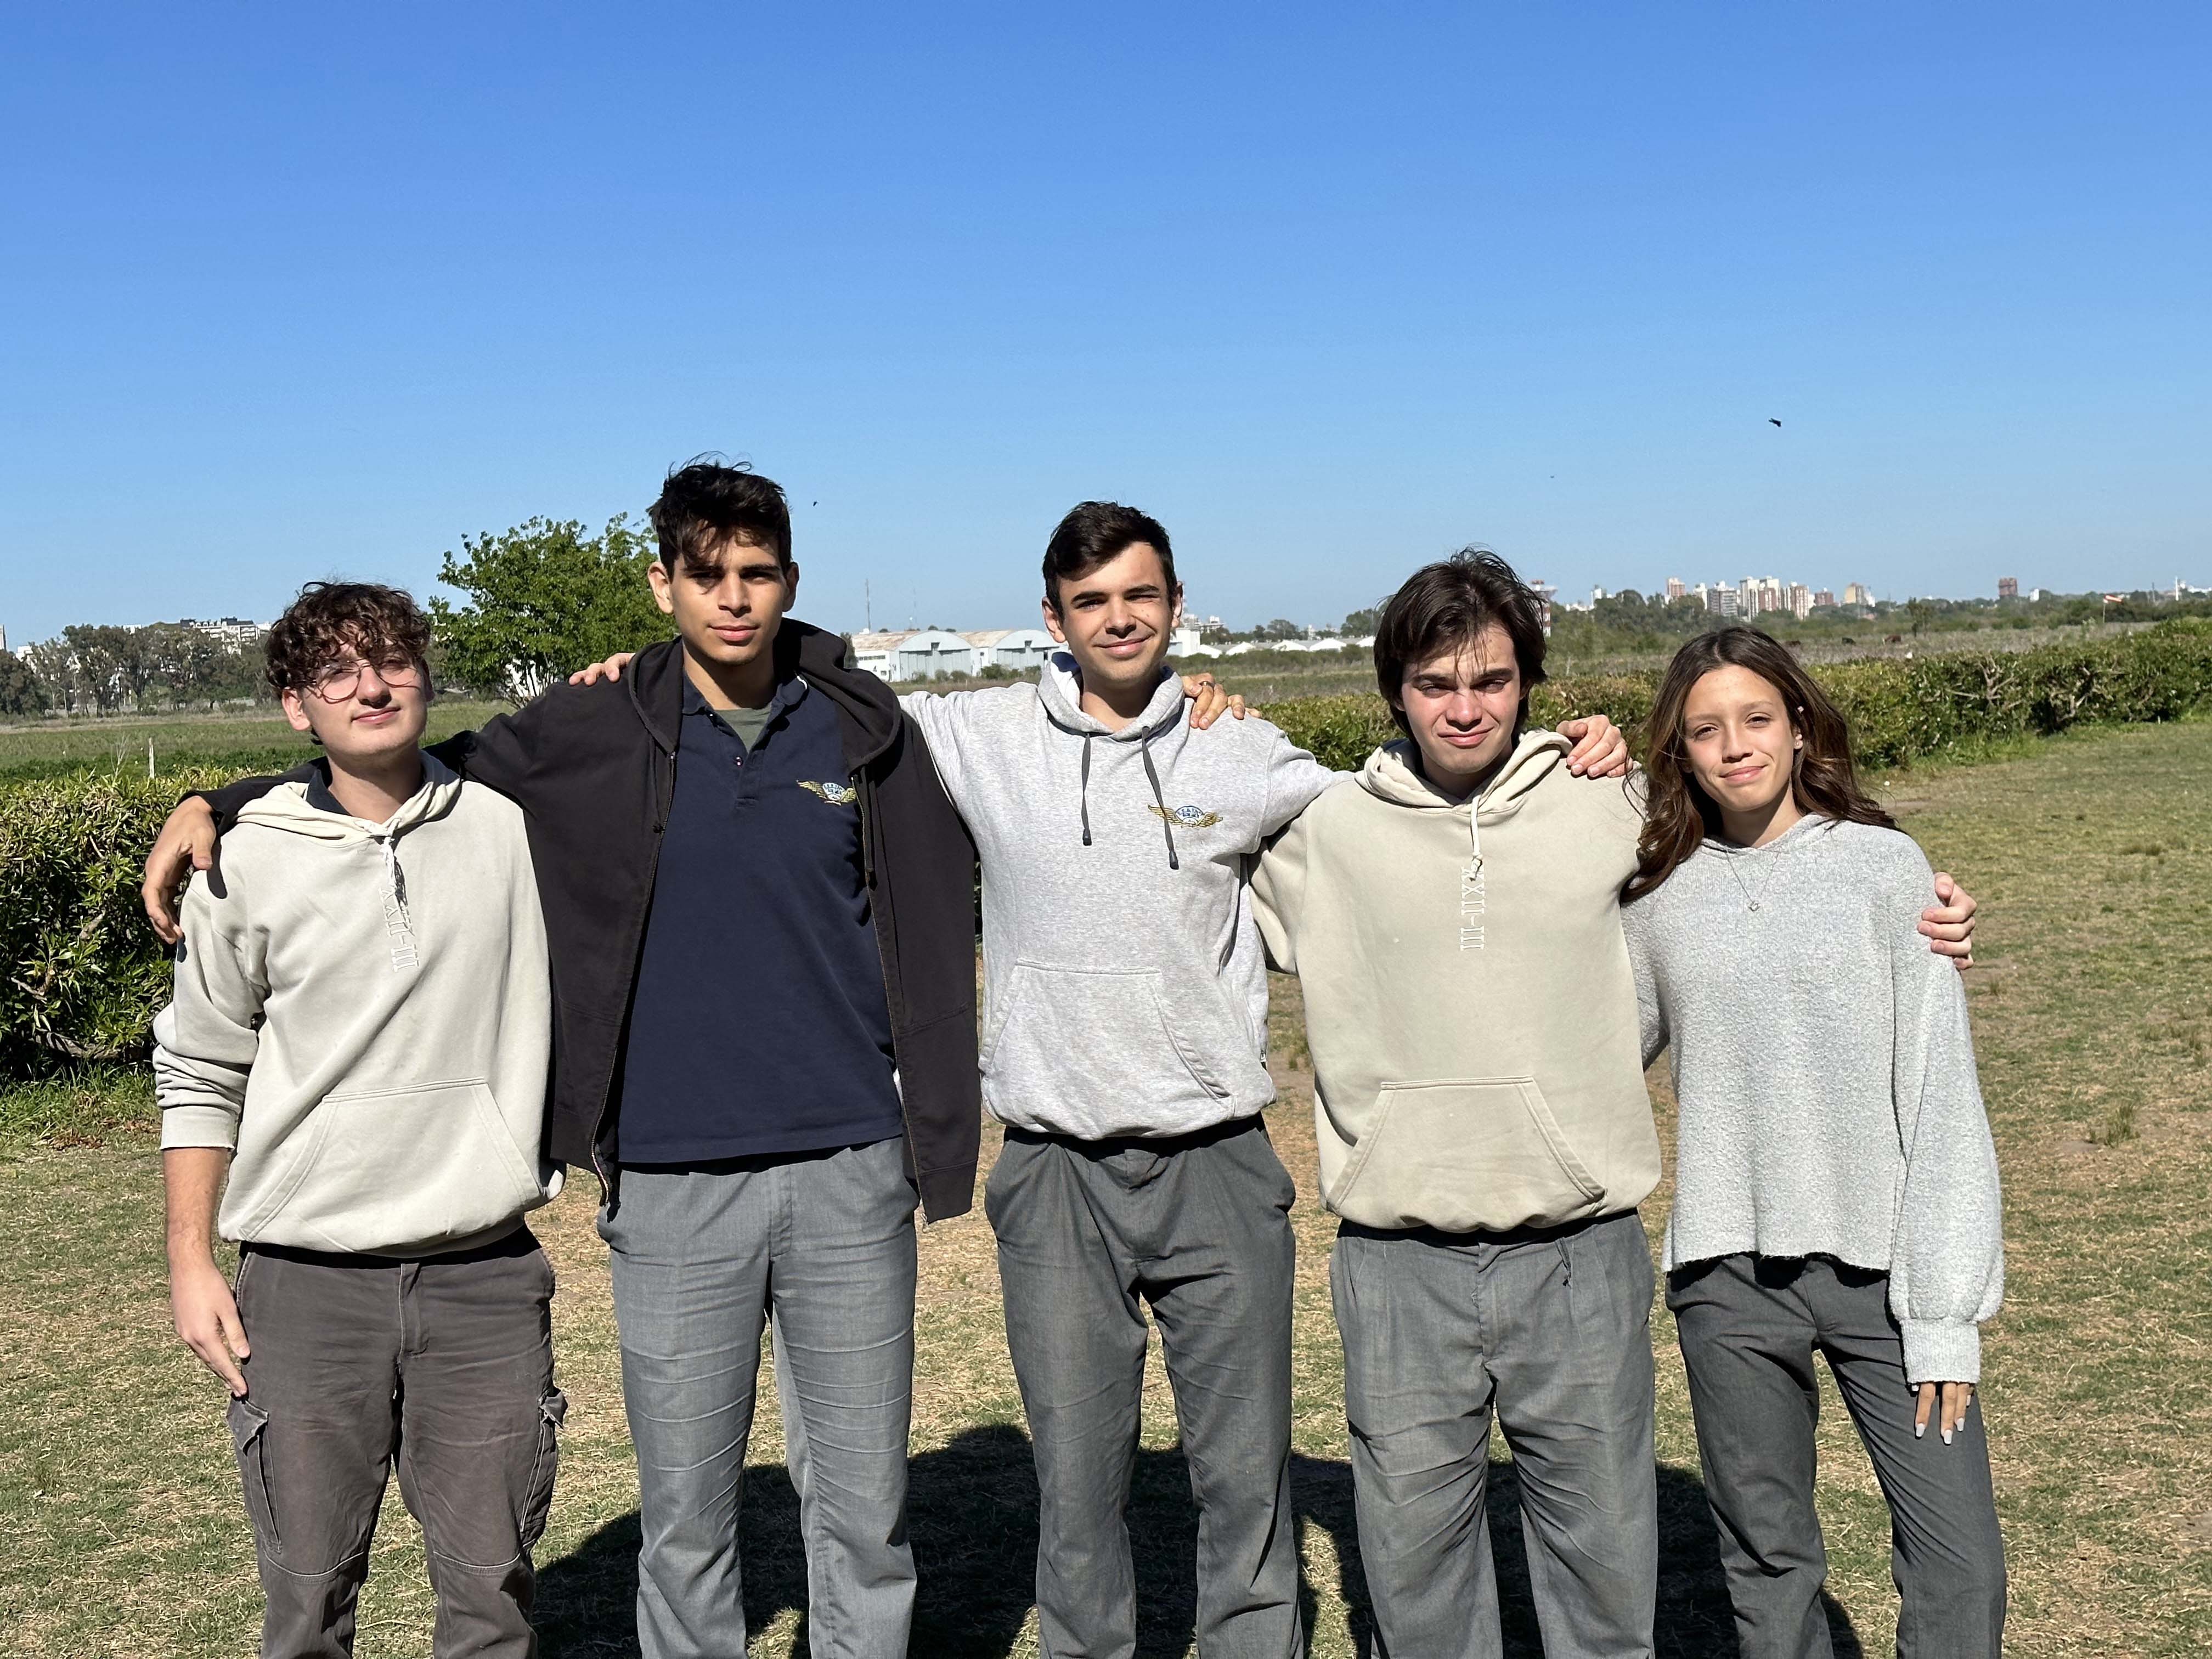
\includegraphics[width=0.85\linewidth]{preambulo/IMG_9428.jpg}
    \caption{Equipo Solar Link}
    \label{fig:equipo solar}
\end{figure}

\begin{figure}[H]
    \centering
    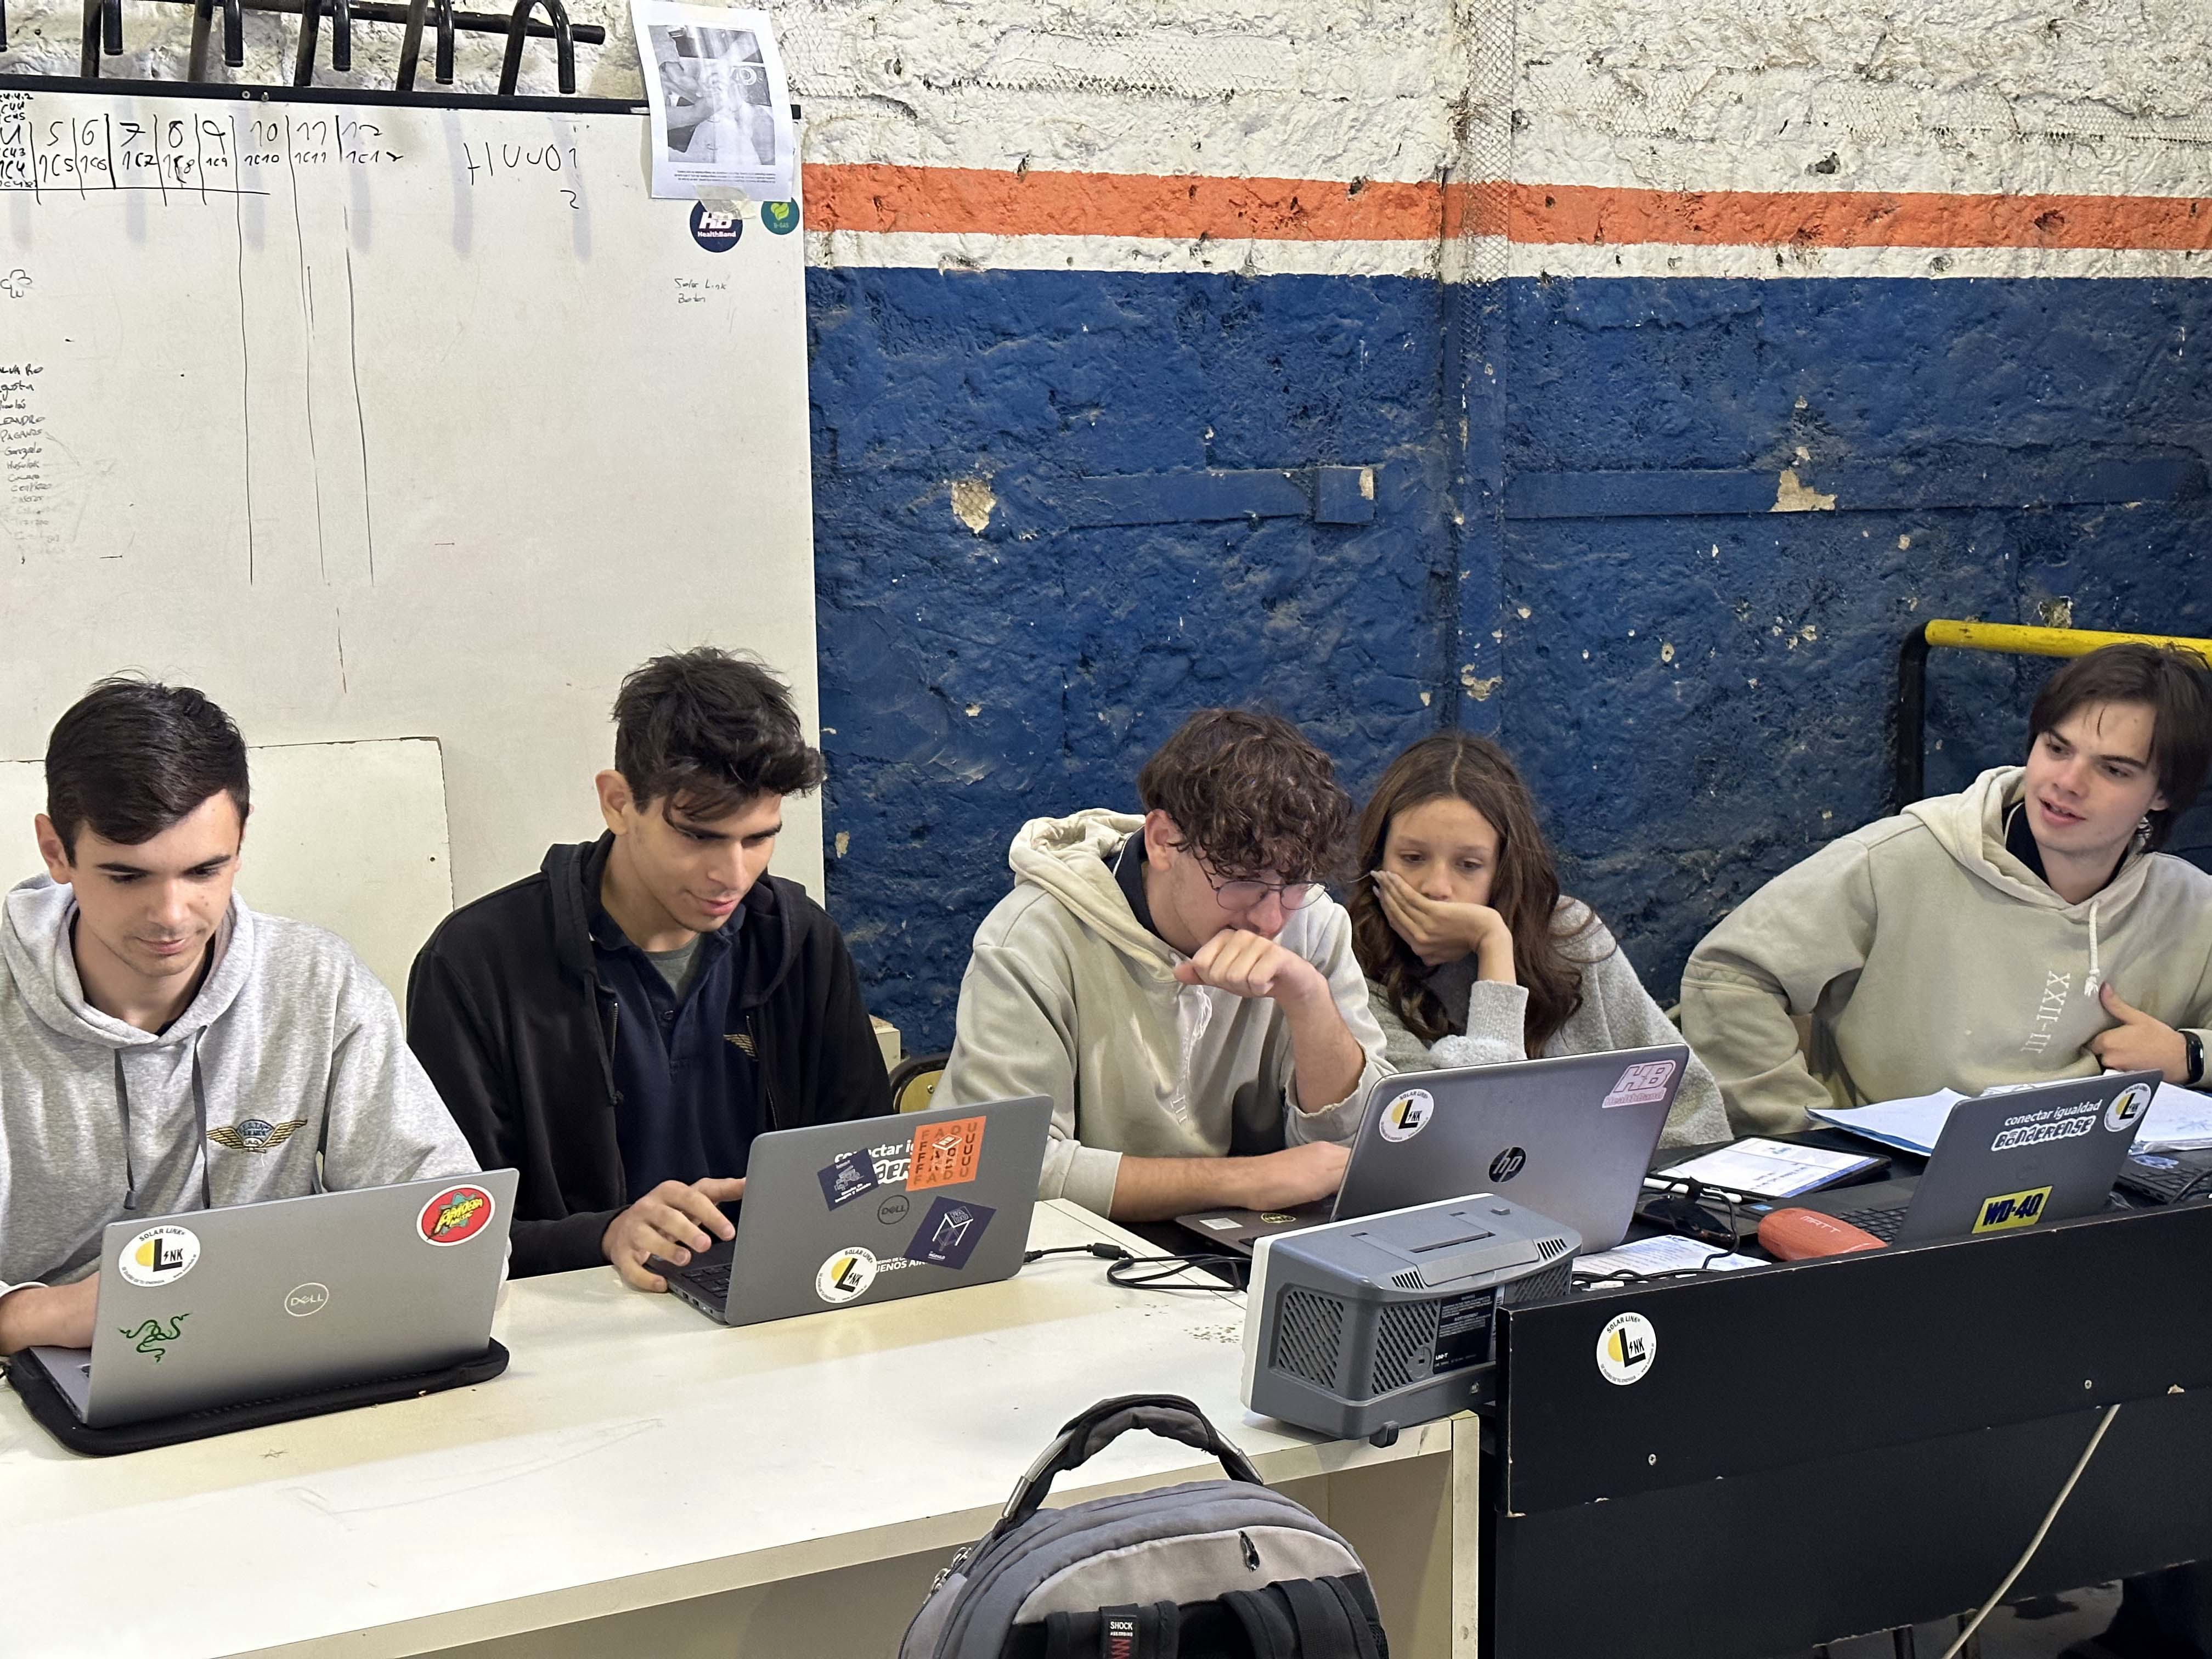
\includegraphics[width=0.85\linewidth]{preambulo/IMG_9439.jpg}
    \caption{Equipo Solar Link trabajando}
    \label{fig:equipo solar laburando}
\end{figure}

\clearpage

\subsection{Contacto}
Podes encontrar a Solar Link en:

\begin{itemize}
\item Mail: info@solarlink.ar
\item Pagina Web: \href{https://www.solarlink.ar}{www.solarlink.ar}
\item Instagram: \href{https://www.instagram.com/solarlink.ar/}{www.instagram.com/solarlink.ar/}
\item Github: \href{https://github.com/solarlink-ar/solarlink}{github.com/solarlink-ar/solarlink}
\item Trello: \href{https://trello.com/w/2023_721c_solarlink}{trello.com/w/2023\_721c\_solarlink}
\end{itemize}

\subsection{Docentes a cargo}

\begin{itemize}
\item Sergio Medina \\ Nos fue de ayuda a la hora de organizar y presentar nuestro proyecto.
\item Fabrizio Carlassara \\ Nos guió en el desarrollo de todo el software del proyecto. 
\item Diego Palmieri \\ Nos prestó las herramientas y los medios necesarios a fin de confeccionar el proyecto.
\end{itemize}

\subsection{Información adicional}

\subsubsection{Tiempo invertido}

\begin{itemize}
\item Fecha de inicio: 20 de noviembre de 2022.
\item Duración: 32 semanas de trabajo.
\item Esfuerzo del proyecto individual: 8 horas de trabajo semanales de cada integrante.
\item Esfuerzo total del proyecto: 1280 horas de trabajo.
\end{itemize}

\subsubsection{Programas utilizados}

\begin{itemize}
\item Visual Studio Code: Fue utilizado como editor de código en diferentes lenguajes.
\item Thonny: Fue utilizado como editor de código para el mirocontroladoor ESP32.
\item KiCad: Fue utilizado para el diseño de todas las PCBs.
\item AutoCad: Fue utilizado para el diseño 3D de las carcasas de las PCBs.
\item Git: Fue utilizado para manejar el código del proyecto entre el grupo.
\item DB Browser: Fue utilizado para leer la base de datos y probar su interacción con lo que programamos.
\item Photoshop: Fue utilizado para el diseño de diferentes imagenes descriptivas del proyecto.
\item Overleaf: Fue utilizado para la realización de la carpeta técnica, de campo y de usuario en LaTex.
\end{itemize}

\subsubsection{Lenguajes de programación y frameworks utilizados}

\begin{itemize}
\item Python: Lógica de página web.
\item MicroPython: Programación del microcontrolador ESP32.
\item C: Programación del microcontrolador Raspberry Pi Pico.
\item Django: Back-end de página web.
\item Microdot: Web de configuración de la ESP32.
\item HTML, CSS: Front-end de la página web.
\item javascript: Front-end de la página web.
\item Terminal de Linux: Manejo de hosting de la web y propósito general.
\item LaTex: Confección de PDFs para carpeta técnica, de campo, y de usuario.
\end{itemize}

\subsection{Agradecimientos}
Este proyecto no hubiera sido posible sin la colaboración de los docentes anteriormente mencionados, la Asociación Cooperadora IMPA y las empresas Eléctrica Bernal, \href{www.bateriasroverano.com.ar}{Roverano}, \href{www.exo.com.ar}{Exo} y \href{www.newtonmicroscopios.com}{Newton Microscopios}.


\section{Introducción}

\subsection{Resumen del proyecto}
Solar Link es un administrador inteligente de energía eléctrica (Smart Grid) que busca maximizar el uso de energías renovables. A través de paneles solares, y con un sistema inteligente, alimentar todo el consumo hogareño posible con energía solar, “switcheando” las líneas de la casa (ejemplo iluminación, tomacorrientes) entre la línea eléctrica del proveedor (edesur p/ej) y la alimentación renovable.\\

Nuestro proyecto es, en esencia, una combinación de los desarrollos en ingeniería eléctrica más reciente (con un hincapié en renovables), y nuestros conocimientos de electrónica e informática. Además, Solar Link estará vinculado a una app y una web para que el usuario pueda ver, controlar y configurar su consumo.\\

Por ejemplo, en una casa el router, la televisión u otros electrodomésticos de uso común que poseen un bajo consumo, pueden ser alimentados con una red solar económica sin problema, pero si a estos consumos se les suman electrodomésticos de alto consumo como lo pueden ser microondas, pavas eléctricas, aires acondicionados, ya no se podrían alimentar por este medio.\\

Por eso, la propuesta de Solar Link es medir constantemente el consumo hogareño, y monitorear si el consumo es lo suficientemente bajo como para ser alimentado por una red de energía solar, o si es demasiado alto como para esta. Dependiendo de esto, el sistema elegirá si la alimentación de la casa será de energía solar o del proveedor de energía eléctrica convencional, conmutando entre estas dos fuentes de energía.\\

En caso de cortes de suministro de luz, Solar Link puede encargarse de lo esencial de la casa que haga falta alimentar, siempre que esté en su margen de funcionamiento.\\

Por otro lado la aplicación web, vinculada con el tablero del usuario, puede mostrarte el consumo hogareño en tiempo real, cuánto consumiste de cada origen y ahorraste en el último tiempo, cuánto significa eso de precio en la factura de luz. También predicciones de la eficiencia de los paneles según el clima presente y futuro. Por último configurar el tablero según la cantidad de baterías o paneles solares y su capacidad.\\

Por último, el proyecto plantea ser modular y versátil, de forma tal que el tablero puede trabajar con cualquier cantidad de paneles o baterías que se le suministren: Solar Link no está limitado sólo a una fuente de energía solar. Aunque el enfoque de nuestro proyecto es aprovechar este tipo de energía, el sistema permite aprovechar también cualquier tipo de fuente: desde una red de proveedor extra, pasando por cosas como un grupo electrógeno, y hasta otras fuentes renovables; biogas, eólica, etc.\\

\subsection{¿Por qué Solar Link?}

\subsubsection{El aspecto de energías no renovables}

Las principales fuentes de energía con las que cuenta hoy el mundo, petróleo, gas natural y carbón mineral, son de carácter no renovable o convencional; es decir que a medida que se van consumiendo disminuyen sus reservas sin posible reposición, salvo que se descubran nuevos yacimientos.\\

Este sector de energías convencionales sigue teniendo un papel protagónico en la matriz energética mundial, producto de un mercado con muchos años de desarrollo tecnológico, con un gran capital hundido en infraestructura, costos competitivos y con porcentajes de rendimiento y de potencia firme superiores a las renovables. Sin embargo, el consumo de combustibles de origen fósil tiene un efecto muy negativo para el medio ambiente, ya que el dióxido de carbono que se produce por su combustión es el principal constituyente de lo que se conoce como gases de efecto invernadero, principales responsables del calentamiento global.\\

Las consecuencias de este efecto son, por ejemplo, el aumento de las temperaturas, los picos de temperaturas extremos, que han venido manifestándose en los últimos años. Es por ello, que las emisiones globales de carbono continúan aumentando, lo que indica la necesidad de un conjunto integral de medidas políticas para lograr la reducción sustancial de las emisiones de carbono.\\

\begin{figure}[H]
    \centering
    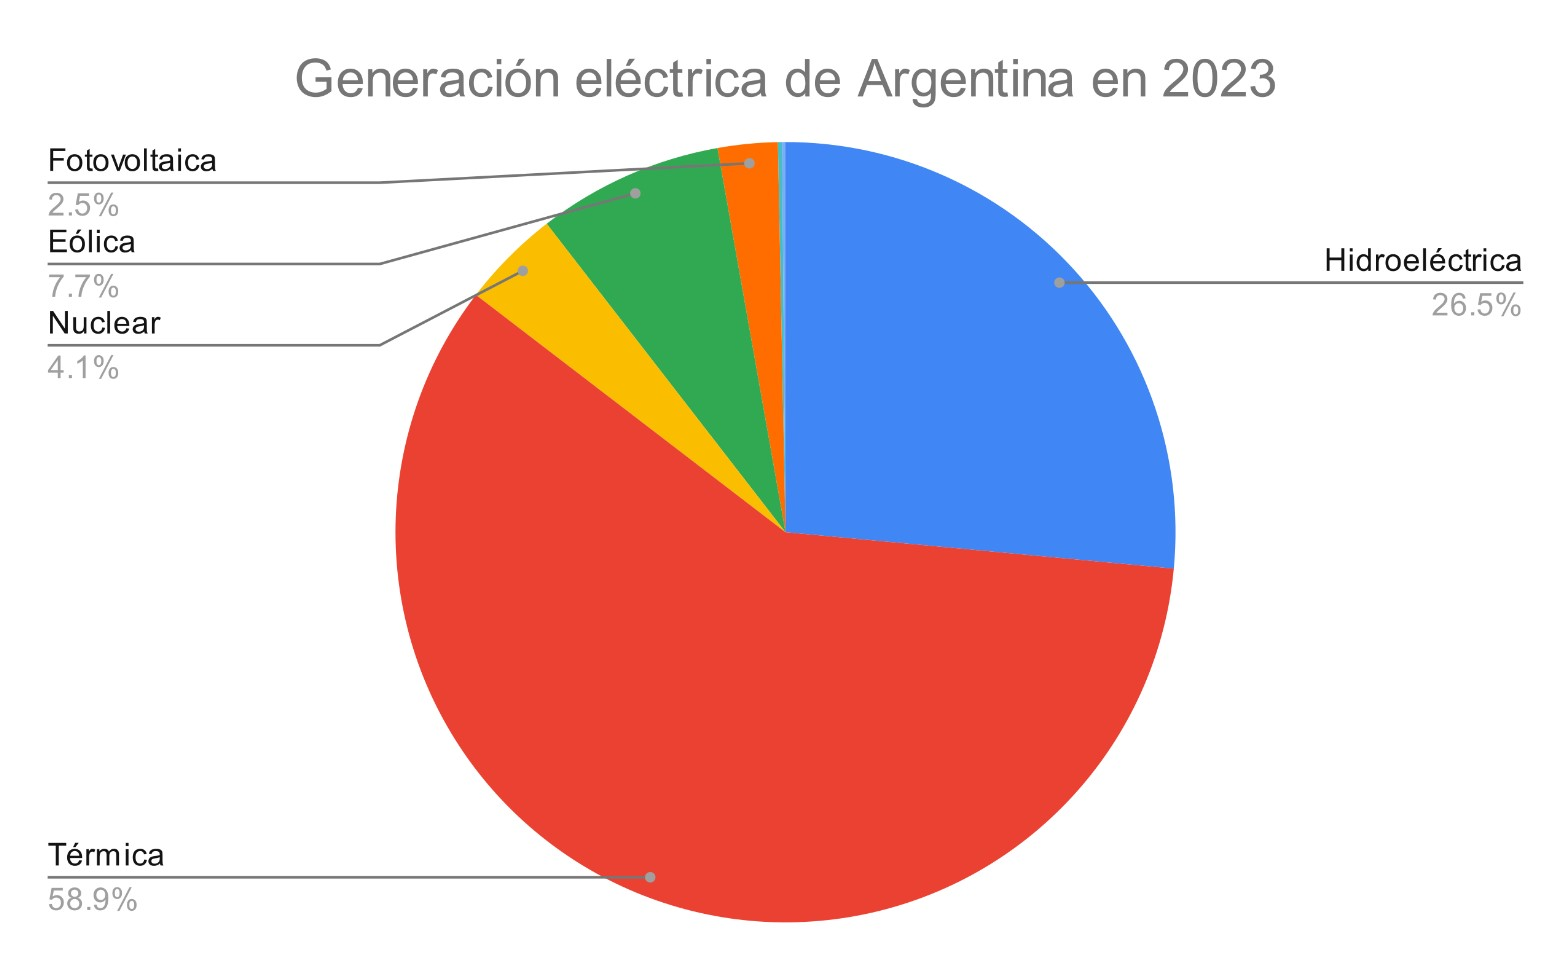
\includegraphics[width=0.85\linewidth]{Intro/Screenshot_20.jpg}
    \caption{Matriz de generación energética en Argentina}
    \label{fig:matriz-energias}
\end{figure}

En Argentina, casi el 60\% de la energía producida y distribuida en el país son de carácter no renovable. La visión de Solar Link es aportar a que esta brecha vaya disminuyendo hasta su exterminacion, volviendo a las energías renovables cabecillas en la generacion de energia. \\

\subsubsection{El aspecto de la energía solar}
Considerando el contexto geográfico y ambiental del país en cuanto a energías renovables, Argentina es un escenario ideal para aplicarlas. Sin embargo, al ver la matriz energética eléctrica de nuestro país, esto no se aprovecha.

\begin{figure}[H]
\centering
\begin{subfigure}{0.4\textwidth}
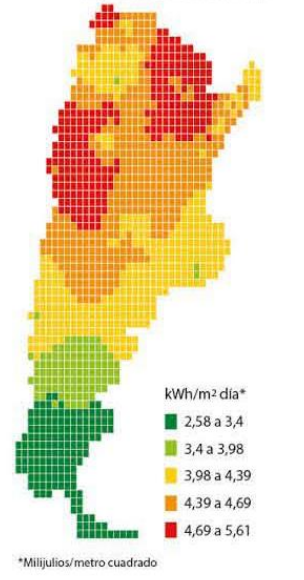
\includegraphics[width=1\linewidth]{Intro/Screenshot_1.png} 
\caption{Zonas del país con mayor \\promedio de intensidad de \\radiación solar}
\end{subfigure}
\begin{subfigure}{0.4\textwidth}
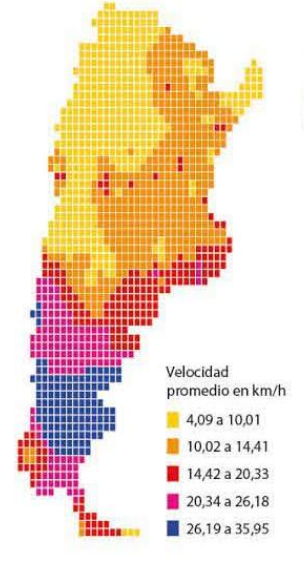
\includegraphics[width=1\linewidth]{Intro/Screenshot_2.png}
\caption{Zonas del país con mayor \\promedio de intensidad de \\los vientos}
\label{fig:subim2}
\end{subfigure}
\label{fig:image2}
\end{figure}

Nótese que justamente las provincias con más potencial solar (inclusive eólico) son aquellas donde el consumo de energía eléctrica es mucho más caro en comparación con el gran Bs. As. y otros centros urbanos, principalmente por los altos costos de distribución de energía. Acá es donde Solar Link tendría su mayor aprovechamiento.\\

Considerando la estadística mostrada, un metro cuadrado de panel solar (en Bs. As.) podría generar 4 kW/h por día. Suponiendo que el panel está en uso 12hs por día, se generan 330 W/h por metro cuadrado de panel. 
En realidad, los paneles son menos eficientes que esto, por tanto para recibir esos 330W/h los paneles son más grandes que 1 metro cuadrado. \\

Sabiendo esto, usaremos como ejemplo un panel solar de 380 W/h y 1.75 metros cuadrados. Por tanto durante, en promedio, 12 hs, se recibirán 380 W/h en el panel. Esta generación de energía implica que por día se producen 4.56 kW/h.\\

En promedio, por mes, una casa de núcleo familiar consume 600 kW/h, o sea 20 kW/h por día. Si hacemos números, nos da que el sistema sería capaz de alimentar con energía solar el 25\% de esa carga (en promedio), ya que de los 600 kW/h por mes, 140 pudieron generarse con el sistema para cargar las baterías y que estas después alimenten las líneas competentes. 
Todo esto solo puede lograrse con una red inteligente.\\

\subsubsection{El aspecto de la red inteligente o Smart Grid}
Sin embargo, un gran problema de la energía solar es su baja eficiencia. La gran mayoría de las veces, al instalar una red eléctrica solar que sea capaz de dar abasto a todo el consumo sería una inversión millonaria. Solar Link busca, a través de una implementación a escala hogareña de un smart-grid, reducir los costos de instalación y mantenimiento, con un enfoque particular en el ahorro a largo plazo.\\

Un smart-grid, o red inteligente, incluye todas las etapas desde la generación, la distribución, y el consumo de energía eléctrica. El objetivo de una red inteligente es descentralizar la red eléctrica para lograr el aprovechamiento eficiente de la energía a través de la electrónica y las tecnologías de información.

\begin{figure}[H]
    \centering
    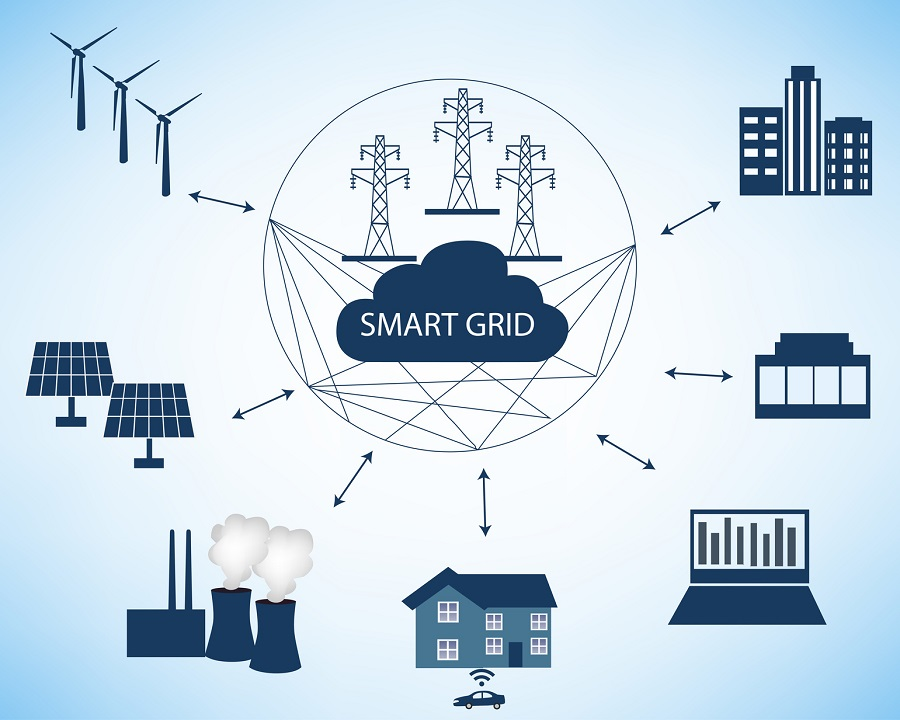
\includegraphics[width=0.75\linewidth]{Intro/smart-grid-2.jpg}
    \caption{Concepto de un smart-grid}
    
\end{figure}
Actualmente, el sistema eléctrico argentino emplea una red tradicional. El proceso desde la generación hasta la distribución está completamente centralizado y engloba casi todo el país en una red única. Como la transición a una smart grid a nivel nacional tardaría varios años (y tampoco está garantizada, siquiera), Solar Link implementa una versión a escala del concepto aprovechando fuentes de energía renovables: en nuestro caso, energía solar.\\

Con una implementación localizada del sistema, Solar Link alterna de manera modular entre el on-grid, que es la red eléctrica común, y el off-grid, que es todo el sistema no conectado a la red principal, lo cual incluye la fuente de energía solar. Al monitorear constantemente los parámetros de consumo generales de la casa, y los consumos provenientes de cada fuente de energía, se puede considerar a Solar Link como un sistema smartgrid.\\

Para completar el esquema de una red inteligente, Solar Link posee conexión a internet, que permitirá al usuario controlar desde su dispositivo los valores de consumo de la casa en el momento, y, utilizando los valores oficiales de tarifas eléctricas, ayudar al consumidor a tomar consciencia de su nivel de consumo y lo que deberá pagar. \\


\subsubsection{Beneficio económico}

Solar Link propone el uso de un sistema solar off-grid, el cual es la alternativa mas económica que se consigue de energía solar. Este sistema consta de panel/es solar/es, batería/s, nuestro cargador MPPT de 3 etapas y un inverter. \\

El sistema que recomendamos instalar en un hogar promedio en Argentina, se compone de dos paneles solares de 380W, un inverter de 2000W, dos baterías de ciclo profundo de 110Ah, el cargador MPPT de 3 etapas de Solar Link, y el módulo Solar Link, con un costo total aproximado de esto ARS \$1.600.000 (USD \$1.600).\\

Mientras tanto, un sistema comparable on-grid, puede salir ARS \$5.000.000 (USD \$5.000). Esto depende del servicio que se contrate y de la empresa que lo realice.\\

No está de más mencionar que al uno producir la energía  que consume, se disminuye el consumo de energía de terceros, el del proveedor eléctrico. Esto quiere decir, que todos los meses se verá reducido el precio que hay que pagar por el suministro de energía eléctrico.\\

El ahorro en este caso no es lineal. Si uno termina consumiendo a fin de mes la mitad de energía que consumiría normalmente, por como funciona el sistema de cobros de las empresas distribuidoras en Argentina, no pagaría la mitad, sino que bastante menos.\\

Esto ocurre porque las empresas establecen un precio para cada KW/h dependiendo de la escala en donde se consuma. Por ejemplo, entre 0KW/h y 200KW/h tiene un precio asignado, entre 200KW/h y 400KW/h otro mayor, y si se exceden esos 400KW/h otro inclusive mayor (estas escalas dependen de la empresa a cargo del suministro eléctrico).\\

Osea, digamos, que cada KW/h entre 0KW/h y 200KW/h valga 1, entre 200KW/h y 400KW/h, 1,5, y si es mayor a 400KW/h, 2. si uno consume 600KW/h, estaría pagando 900, mientras que si uno consume 300KW/h, estaría pagando 350, bastante menos de la mitad. Este ejemplo ilustra como funciona el sistema de cobros de las compañías distribuidoras en Argentina. Las escalas y los valores son a modo de ejemplo. Pueden ser diferentes segun la empresa, la región, y el momento en donde se analice.\\

\subsubsection{Incentivo y concientización}

A través de nuestra aplicación, el usuario tendrá acceso a toda la información que respecta al consumo eléctrico de su casa. Esto le permite conocer al detalle no solo el consumo total, sino tambien el consumo que generó el sistema solar propio.\\

Esto genera en el usuario un sentido de ganancia y de gasto propio. Saber bien cuanto se esta gastando, porque y cuanto de este gasto se amortiguo ayuda a concientizar sobre el consumo de energia en general. \\

Mas allá del gasto de energía, tener un sistema que, ya sea de manera directa o indirecta, ayuda al medio ambiente, tiene un efecto positivo para la psiquis y para el entorno donde uno vive. Saber que uno esta aportando su grano de arena (siendo el mismo economicamente viable y rentable) genera tranquilidad y un sentido de responsabilidad ciudadana. \\

\subsection{Alcance}

Solar Link está destinado principalmente al mercado doméstico argentino, el cual, al día de hoy, está sufriendo de constantes aumentos en la factura de luz. Esto no solo genera un incentivo en el ahorro energético, sino que también convierte a Solar Link en un servicio cada vez mas redituable para el usuario final. \\

Sin embargo, nuestro proyecto tambien puede ser utilizado en cualquier instancia donde se quiera instalar un sistema solar. Puede ser una fábrica, una oficina, un departamento, un quincho, donde se quiera. Los únicos requisitos son tener acceso a la red eléctrica y luz solar a disposición.\\

\subsection{Estado del arte}

Actualmente, en el mercado argentino, existen principalmente tres tipos de instalaciones de energía solar para un hogar. Cada tipo cuenta con sus propias ventajas y desventajas:\\

\begin{table}[H]
\begin{tabular}{|l|l|l|}
\hline
Tipo     & Ventajas                                                                                                                 & Desventajas                                                                                            \\ \hline
On-Grid  & \begin{tabular}[c]{@{}l@{}}Sistema acoplado a la línea doméstica\\ Alimenta casi el 100\% con energía solar\end{tabular} & \begin{tabular}[c]{@{}l@{}}Alto costo\\ Desperdicio de energía\end{tabular}                            \\ \hline
Off-Grid & \begin{tabular}[c]{@{}l@{}}Económico\\ Acumula energía\end{tabular}                                                      & \begin{tabular}[c]{@{}l@{}}Requiere una línea exclusiva \\ para este sistema\end{tabular}              \\ \hline
Híbrido  & \begin{tabular}[c]{@{}l@{}}Sistema acoplado a la línea doméstica\\ Acumula energía\end{tabular}                          & \begin{tabular}[c]{@{}l@{}}Potencia limitada\\ Requiere instalación especial\end{tabular} \\ \hline
\end{tabular}
\end{table}

Los sistemas \textbf{on-grid}, como su nombre lo indica, se instalan directamente en la línea de la casa. Toda la energía que producen los paneles se entregan a la línea general de la casa, sin almacenarse en ningún lado. Si la casa consume mas que lo que generan los paneles, se consume la energía correspondiente a este exceso del proveedor eléctrico, y si consume menos, la energía generada por demás se entrega a la red eléctrica del proveedor. \\

Para este tipo de sistemas es necesaria la instalación de un medidor bidireccional, que mide tanto el consumo de la casa como lo que devuelve por el exceso en la producción. Si bien este medidor descuenta lo que uno devuelve a la red eléctrica, lo que uno consume es mas caro, no es muy redituable y no su instalación depende del proveedor de energía eléctrica.\\

Los sistemas \textbf{off-grid}, por otra parte, acumulan la energía generada por los paneles solares en baterías, para luego convertirla en los 220Vac que necesita la casa. El problema de esto, es que la energía extraída de las baterías no se puede incorporar directamente a la línea de la casa, por lo que es necesario la utilización de una línea exclusiva para lo que este sistema genere. Esto implica tener que hacer una instalación eléctrica aislada e independiente del resto de la casa, algo impráctico si además se tiene en cuenta que la utilización de esta línea debe ser controlada y depende directamente de la carga de los paneles.\\

Los sistemas \textbf{híbridos} son sistemas solares off-grid que se incorporan a la línea de la casa. Pueden utilizar tanto la energía solar acumulada como la energía del proveedor eléctrico. Para utilizar este tipo de sistema es necesaria una instalación especial, que se tiene que realizar en líneas dedicadas. Además, por como es su principio de funcionamiento, el sistema solar no es expandible, por lo que la potencia instalada en un principio no podrá modificarse.\\

Mientras tanto, \textbf{Solar Link} busca recopilar todas las ventajas de estos 3 tipos de sistemas solares, y dejar en el camino todas las desventajas posibles. Se podría decir que Solar Link es un sistema que acumula y utiliza energía solar, acoplado a la línea de la casa, económico, modular expandible y amigable con el usuario, compartiendo toda la información necesaria sobre el sistema solar instalado y el consumo de la casa.

\subsection{Síntesis}
Solar Link aprovecha sus cualidades como gestor inteligente para poder aprovechar la energía solar al máximo. Usualmente, la instalación de una fuente de energía solar por sí sóla no daría abasto para toda la casa (recordemos que en nuestro ejemplo sólo cubría el 30\%), y otros tipos de implementación alternativas a una red inteligente serían rígidas e ineficientes. A través de Solar Link, buscamos que con el control automático de consumo y la separación modular de las redes de la casa logremos maximizar la eficiencia en el consumo, y minimizar los gastos posibles.\\

Nuestro objetivo es introducir al país un sistema capaz de evitar energía cuya generación es, en su mayoría, resultado de fomentar el cambio climático, introduciendo energías renovables y control y concientización del consumo a sus usuarios, en otras palabras un smart grid con energías renovables. Por otro lado, otorga a sus usuarios energía generada por ellos mismos para su hogar, y por lo tanto, no deben pagar por ella. \\

Entre sus beneficios están, el uso de energías renovables, la producción de energía en el propio entorno de uso, que reduciría el consumo en la boleta, una aplicación web que permite ver el consumo y configurarlo, dando control al usuario de su consumo y que sea consciente de este. 

\clearpage

\section{Desarrollo técnico}

\subsection{Descripción del funcionamiento}
Nuestra propuesta para solventar algunas desventajas de los sistemas de energía renovable (especialmente la solar) es crear un sistema autónomo e inteligente que, a través de un sistema off-grid, sea capaz de acoplar y desacoplar la casa de la red eléctrica alternativa, dependiendo del consumo de la misma.\\

Este sistema debe ser capaz de leer el consumo de las líneas de la casa, y debe conocer la potencia que el sistema solar instalado puede entregar. De esta manera, cuando se detecte que el consumo de la casa puede ser alimentado por el sistema off-grid, dejará de alimentar la casa con el proveedor de energía eléctrica. Mientras que si el consumo supera el límite establecido, volverá a alimentarla. Para realizar esto, se utiliza la técnica “cruce por cero”, para sincronizar el cambio entre líneas, y que no se note este cambio.\\

Puede ocurrir que en una casa estén constantemente heladeras, calefactores, computadoras, y otros electrodomésticos de alto consumo en uso, y que el sistema off-grid nunca pueda ser capaz de alimentar la línea general de la casa. Para esto, proponemos que Solar Link trabaje parcialmente sobre la casa, pudiendo alimentar independientemente la línea de iluminación y la línea de tomas de la casa. Es decir, si se da el caso mencionado anteriormente, la línea de iluminación seguiría siendo alimentada por energía solar, mientras que la línea de tomas la sería alimentada por el proveedor de energía eléctrica.\\

En caso de un corte de suministro de luz,el sistema Solar Link seguiría funcionando, alimentando a la mayor parte de la casa posible.
Un aspecto clave del proyecto es la accesibilidad e interacción con el usuario. Solar Link incluye una aplicación vinculada con sensores distribuidos en la red eléctrica de la casa. El usuario podrá así tener una noción más concreta de cuáles son los principales consumos del hogar, y le brinda la información necesaria a Solar Link para alternar el uso de energía off-grid y energía de red en cada línea modular.\\

Además, para optimizar la carga del sistema solar, desarrollamos un cargador MPPT de 3 etapas que no solo le da la mejor carga posible a las baterías del sistema, sino que también monitorea el estado de carga de las mismas, y se lo comunica al módulo Solar Link para tenerlo en cuenta a la hora de la conmutación entre líneas, y a la hora de entregarle la mayor cantidad de información posible sobre el sistema al usuario.\\

\subsection{Diagramas de Solar Link}

\begin{figure}[H]
    \centering
    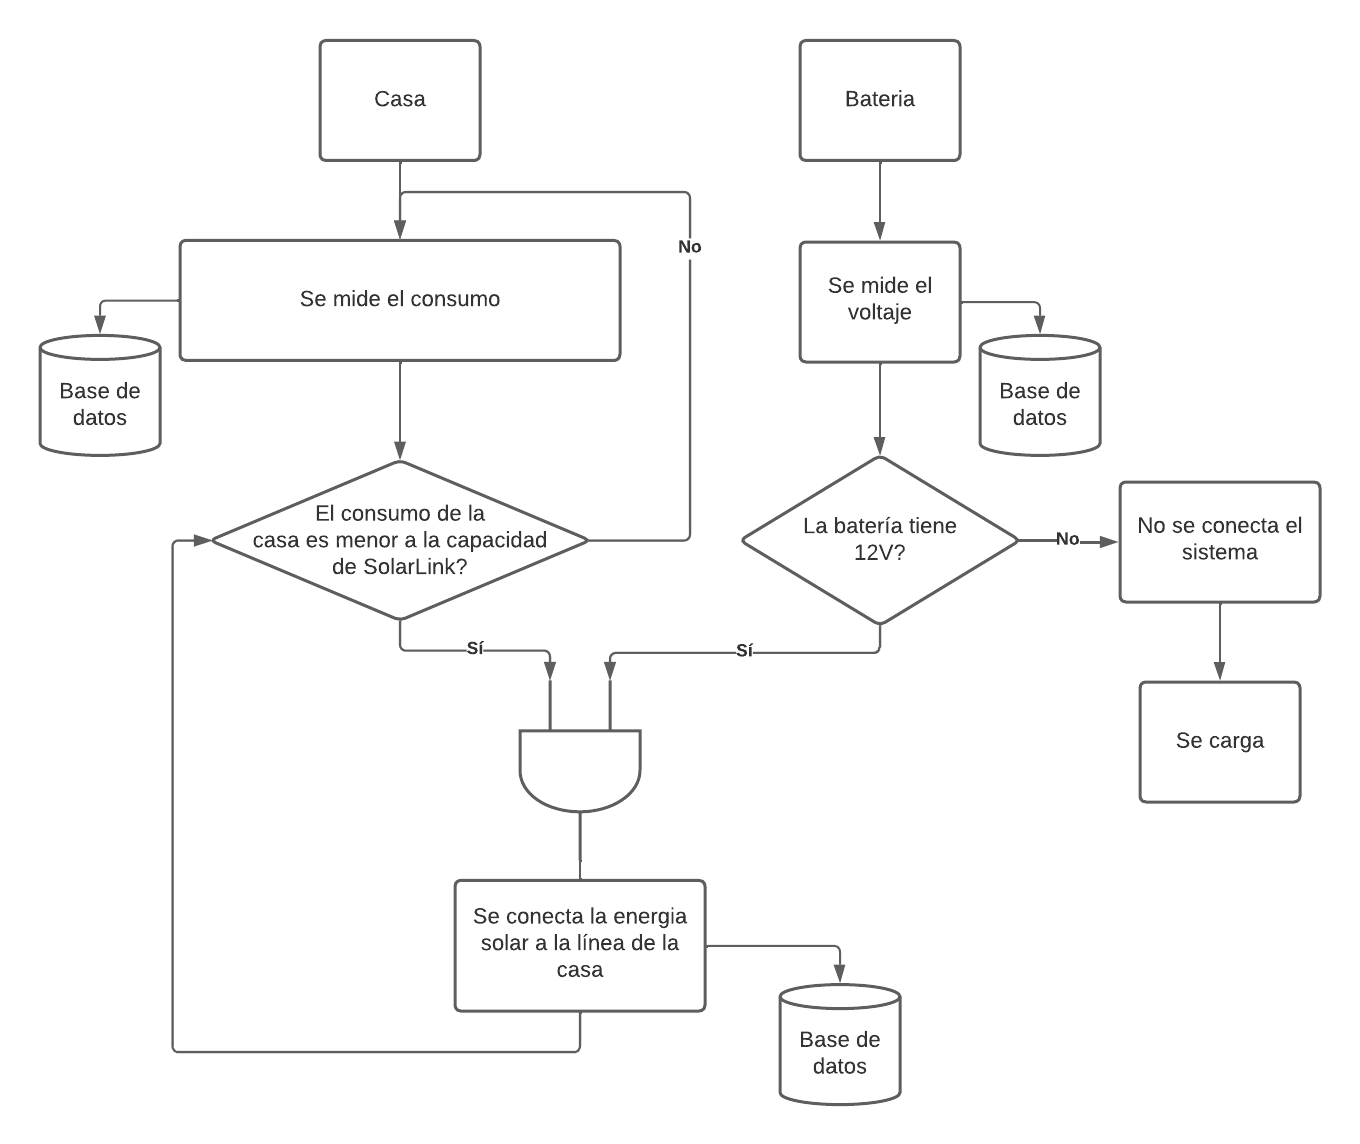
\includegraphics[width=1\linewidth]{analisis-tecnico/Diagrama de flujo SolarLink.png}
    \caption{Diagrama de flujo de Solar Link.}
    \label{fig:enter-label}
\end{figure}

\begin{figure}[H]
    \centering
    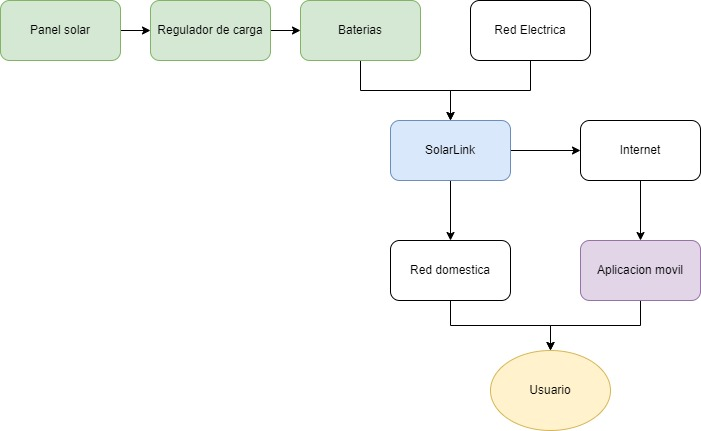
\includegraphics[width=1\linewidth]{analisis-tecnico/Diagrama SolarLink.jpg}
    \caption{Diagrama en bloque del sistema Solar Link.}
    \label{fig:flujo-solarlink}
\end{figure}

\begin{figure}[H]
    \centering
    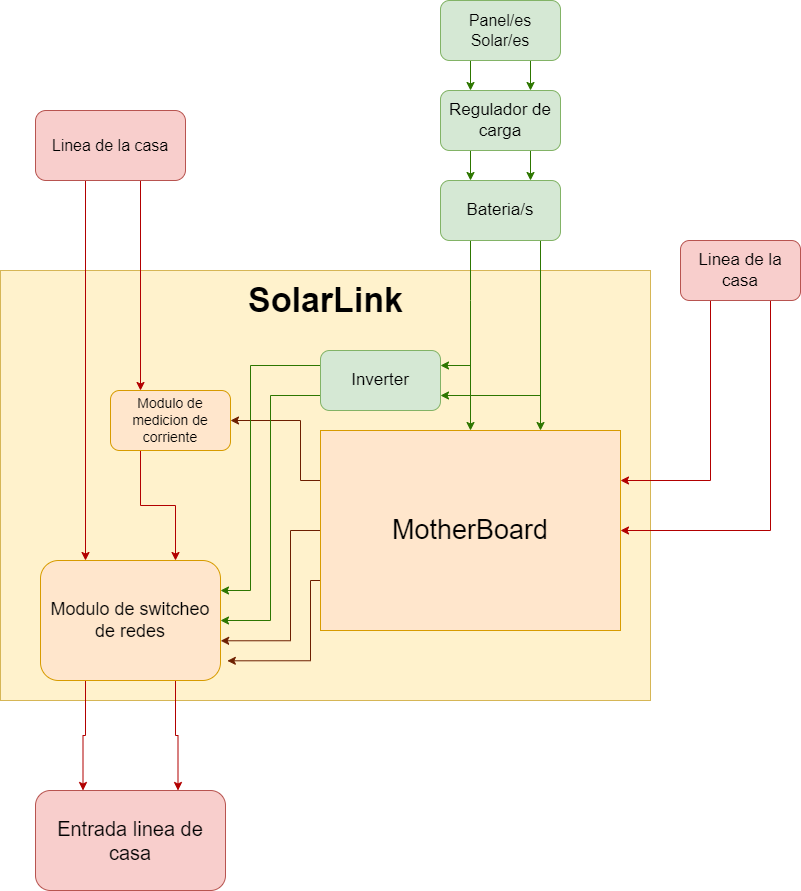
\includegraphics[width=1\linewidth]{analisis-tecnico/Diagrama en bloques.png}
    \caption{Diagrama en bloque del módulo Solar Link.}
    \label{fig:bloque2-solarlink}
\end{figure}

\begin{figure}[H]
    \centering
    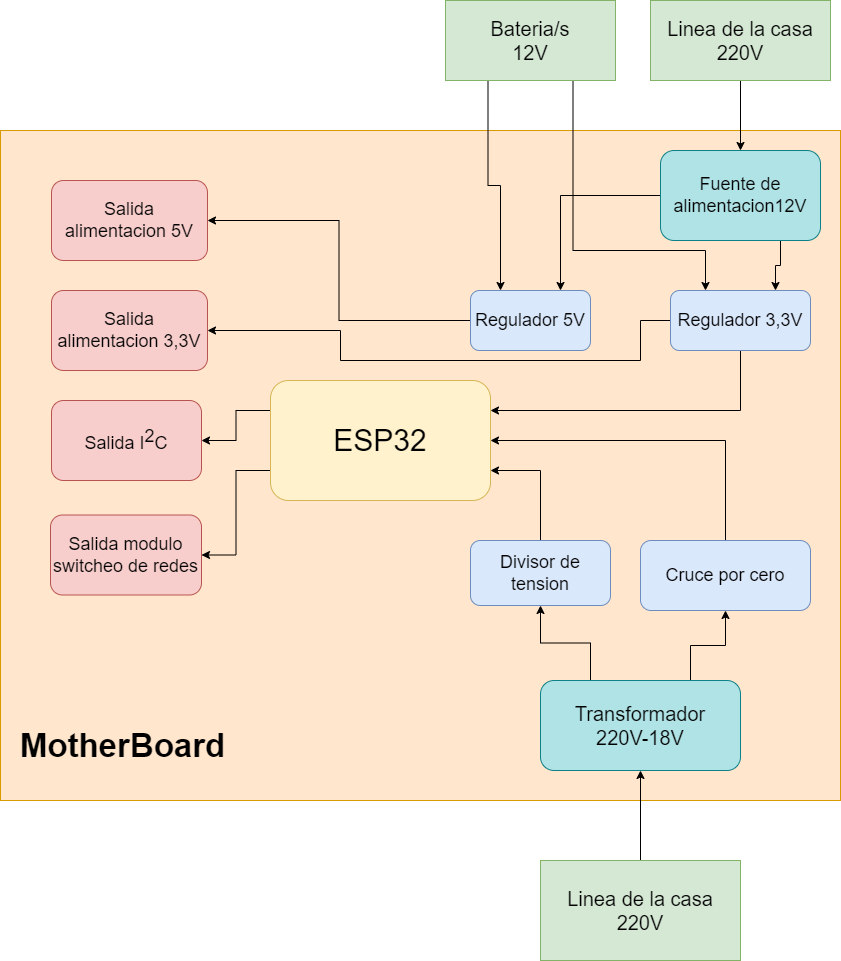
\includegraphics[width=1\linewidth]{analisis-tecnico/Diagrama en bloques mother.png}
    \caption{Diagrama en bloques de la motherboard.}
    \label{fig:diagrama en bloque mother}
\end{figure}

\subsection{Diagramas del cargador MPPT de 3 etapas}

\begin{figure}[H]
    \centering
    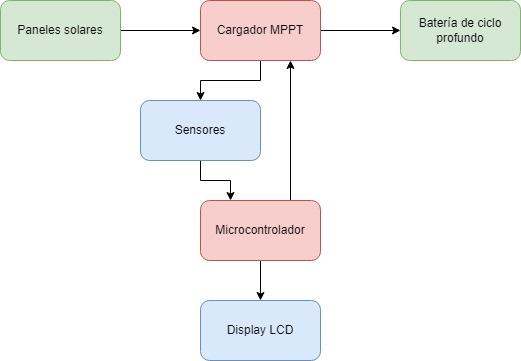
\includegraphics[width=1\linewidth]{analisis-tecnico/Diagrama en bloque MPPT.jpg}
    \caption{Diagrama en bloque del cargador MPPT.}
    \label{fig:diagrama bloque mppt}
\end{figure}

\begin{figure}[H]
    \centering
    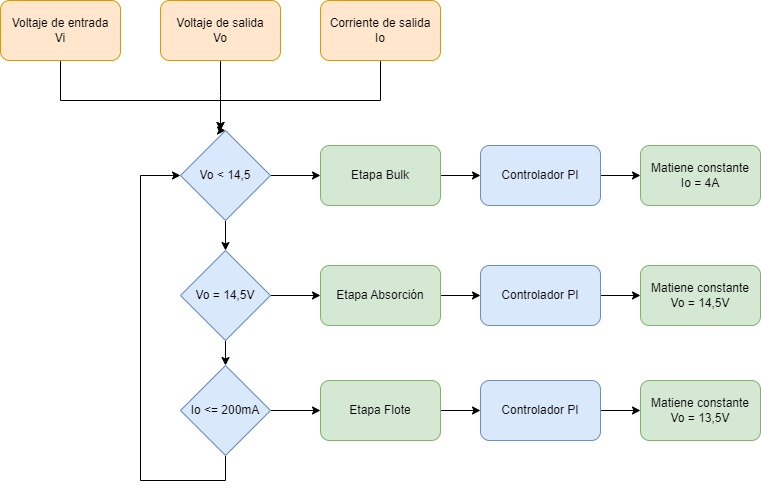
\includegraphics[width=1\linewidth]{analisis-tecnico/Diagrama de flujo MPPT.jpg}
    \caption{Diagrama de flujo del cargador MPPT.}
    \label{fig:diagrama bloque mppt}
\end{figure}

\clearpage

\section{Cargador MPPT de 3 etapas}

\subsection{¿Qué es un cargador MPPT?}

Un cargador MPPT (Maximun Power Point Tracking) es una técnica utilizada para obtener siempre la mayor potencia posible bajo condiciones de alimentación variables, como lo son los paneles solares o las turbinas eólicas, cuya potencia depende de las condiciones climáticas.\\

Los sistemas solares fotovoltaicos poseen relaciones variables de potencia, que dependen de la cantidad disponible de luz solar, sombras, temperatura de los paneles y las características de carga. Cuando estas condiciones varían, la impedancia característica que establece el mayor punto de transferencia de potencia cambia. De esta forma, el sistema es optimizado cuando las condiciones de carga cambian, manteniendo la transferencia de potencia en la mayor eficiencia posible. Este punto de transferencia máximo se llama MPP (maximun Power Point), y, el proceso para conseguirlo, MPPT.\\

\begin{figure} [H]
    \centering
    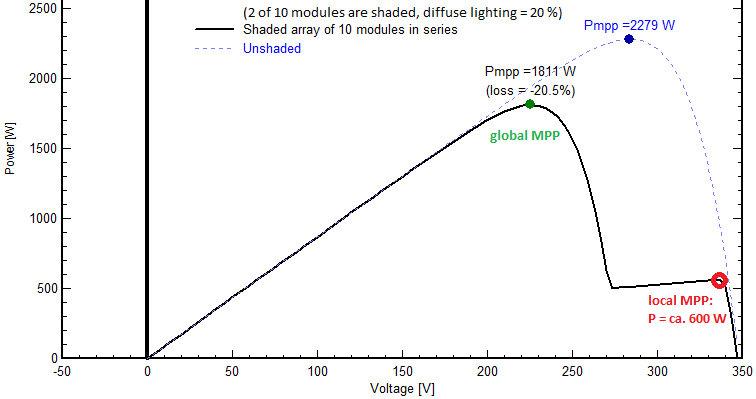
\includegraphics[width=0.95\linewidth]{MPPT/UP-curve_of_partially_shaded_solar_generator.png}
    \caption{Curva de Potencia/Voltaje de un sistema solar parcialmente obscurecido.}
\end{figure}

\subsection{¿Qué son las 3 etapas?}

El cargador MPPT de Solar Link va un paso mas allá, no solo maximizando la transferencia de potencia con pérdidas mínimas, sino que también utiliza 3 etapas diferentes para cargar la batería. Estas etapas se llaman Bulk, Absorción y Flote, las cuales le dan a la batería una carga mas profunda, aumentando su rendimiento y vida útil. \\

La fase \textbf{bulk} le entrega a la batería de manera constante la corriente máxima admitida. En esta fase, la batería se carga hasta un 80\%. Cuando se llega a un cierto voltaje (14,5V), cambia a la fase \textbf{absorción}, donde se mantiene constante este voltaje, y la bateráa llega a cargar el 20\% restante. Cuando el valor de corriente  es menor a un cierto valor (300mA), pasamos a la fase \textbf{flote}, donde se mantiene constante un voltaje menor (13,5V). Esta fase mantendrá la batería cargada cuando no esté siendo utilizada, evitando el desgaste generado en las baterías cuando no se usan por un tiempo.

\begin{figure}[H]
    \centering
    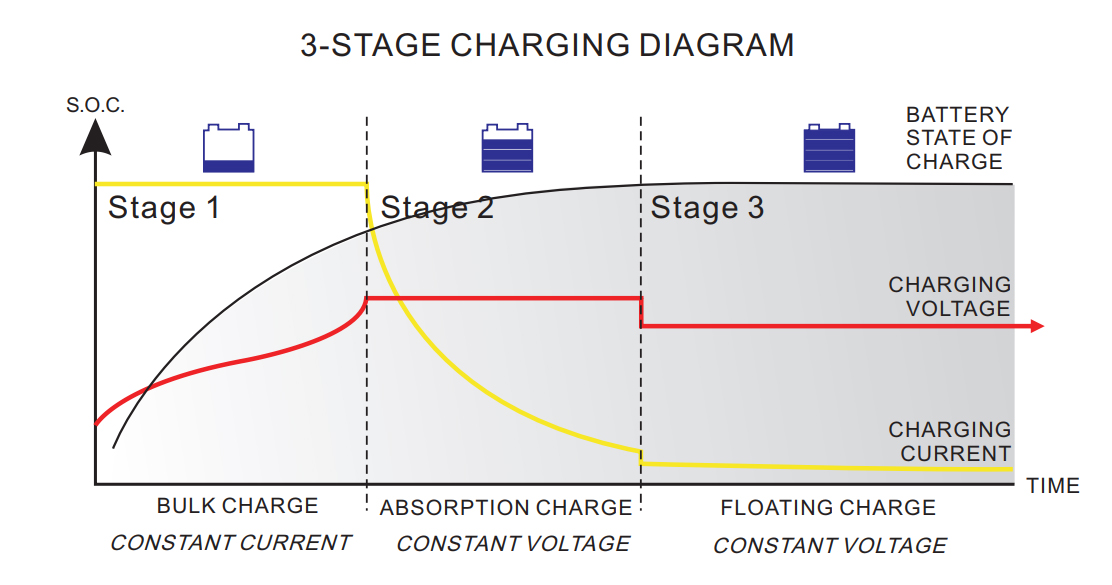
\includegraphics[width=0.95\linewidth]{MPPT/5a9f8145-6356-4504-b0b6-9d73450df4c1.jpg}
    \caption{Gráfica del voltaje, la corriente, y el porcentaje de carga de la batería en el tiempo.}
    \label{fig:grafica-carga}
\end{figure}

\subsection{Principio de funcionamiento}

\subsubsection{Convertidor Buck DC-DC}
Para convertir un voltaje de continua de entrada de mayor valor en uno de menor, existen infinidad de opciones. Por ejemplo, se podría usar un divisor resistivo, donde una resistencia disipa el voltaje que no nos interesa, pero esta opción es muy poco eficaz, porque esa energía disipada son pérdidas considerables, además en nuestro caso se necesita de un sistema que podamos controlar y variar su salida. \\

Ahi es donde entra el convertidor reductor, o convertidor Buck, que a la vez que reduce el voltaje de salida aumenta la corriente de salida, manteniendo constante la potencia. Es una clase de fuente switching, y provee una eficiencia muy alta, por encima de un 90\%. Además, controlando la señal de switching, podemos variar el voltaje de salida a voluntad.

\begin{figure}[H]
\begin{subfigure}{0.5\textwidth}
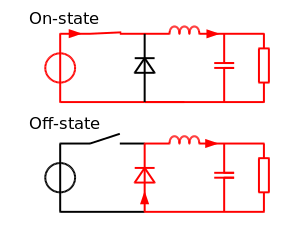
\includegraphics[width=0.9\linewidth]{MPPT/Buck_operating.svg.png} 
\caption{Las dos configuraciones de un \\convertidor Buck, On y Off.}
\label{fig:buck-1}
\end{subfigure}
\begin{subfigure}{0.5\textwidth}

\includegraphics[width=0.9\linewidth]{MPPT/300px-Buck_conventions.svg.png}
\caption{Voltajes, corrientes y nombres de \\los componentes.}
\label{fig:buck-2}
\end{subfigure}

\caption{Convertidor Buck.}
\label{fig:image2}
\end{figure}

Para entender este circuito, se debe hacer un análisis del estado transitorio del mismo en sus dos estados, On y Off. En principio, con el estado Off, la corriente en el circuito es nula. Cuando cambia al estado On, la corriente va empezar a subir y la bobina va a generar una caída de voltaje entre sus terminales. Esta caída de voltaje provoca que el voltaje resultante en la carga sea menor. A medida que pasa el tiempo, el índice de cambio de la corriente disminuye, y el voltaje en la bobina también disminuye, aumentando el voltaje en la carga. Durante este proceso, la bobina almacena energía en forma de campo magnético. \\

Cuando el interruptor de abre de vuelta (Off), la fuente de voltaje se remueve del circuito y la corriente disminuye. Esta corriente decreciente produce una caída de voltaje en la bobina (opuesto al generado en el estado On), y ahora la bobina se convierte en una fuente de corriente. La energía almacenada en el campo magnético de la bobina suporta el flujo de corriente por la carga. Esta corriente, que fluye mientras la fuente de voltaje está desconectada, cuando se suma a la corriente que fluye en el estado On, da como resultado una corriente de salida promedio mas grande que la que entrega la fuente de voltaje.\\

\begin{figure}[H]
    \centering
    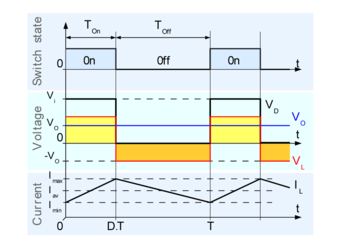
\includegraphics[width=1\linewidth]{MPPT/350px-Buck_chronogram.png}
    \caption{Gráfica en el tiempo del comportamiento de las tensiones y corrientes de un convertidor buck.}
    \label{fig:grafica-mppt}
\end{figure}

Este aumento en la corriente promedio estaría compensando la reducción en el voltaje, manteniendo idealmente la potencia entregada en la carga. Si el switch se abre mientras la corriente sigue aumentando, entonces siempre va a haber una caída de tensión sobre la bobina, por lo tanto la carga siempre tendra menos voltaje que la entrada.\\

\subsubsection{Sistema de control}
Una vez explicado el funcionamiento de la fuente reductora, ahora hay que explicar como se puede hacer para controlar ese voltaje de salida.\\

Si uno logra variar la frecuencia con la que ese switch se abre y se cierra, y al mismo tiempo medir la corriente y la tension recibida en la carga, se puede diseñar un sistema de control que, teniendo en cuenta esas variables, varíe esa frecuencia del interruptor con esas mediciones como realimentación, controlando una o la otra.\\

El sistema de control que utilizamos es un control proporcional integral, o PI, siendo la aplicación de un control proporcional y uno integral al mismo tiempo.\\

La parte proporcional de un control es el producto entre la señal de error ($e(t)$) y la constante proporcional ($K_{p}$). Variando ($K_{p}$) se cambia la velocidad del control. Pero solo con un control proporcional se tiene error en régimen permanente, ya que este tipo de control requiere de error para entregar señal de control. La fórmula matemática que responde a esto es:\\
\begin{equation}
    P_{sal}=K_{p} e(t)
\end{equation}\\

\begin{figure}[H]
    \centering
    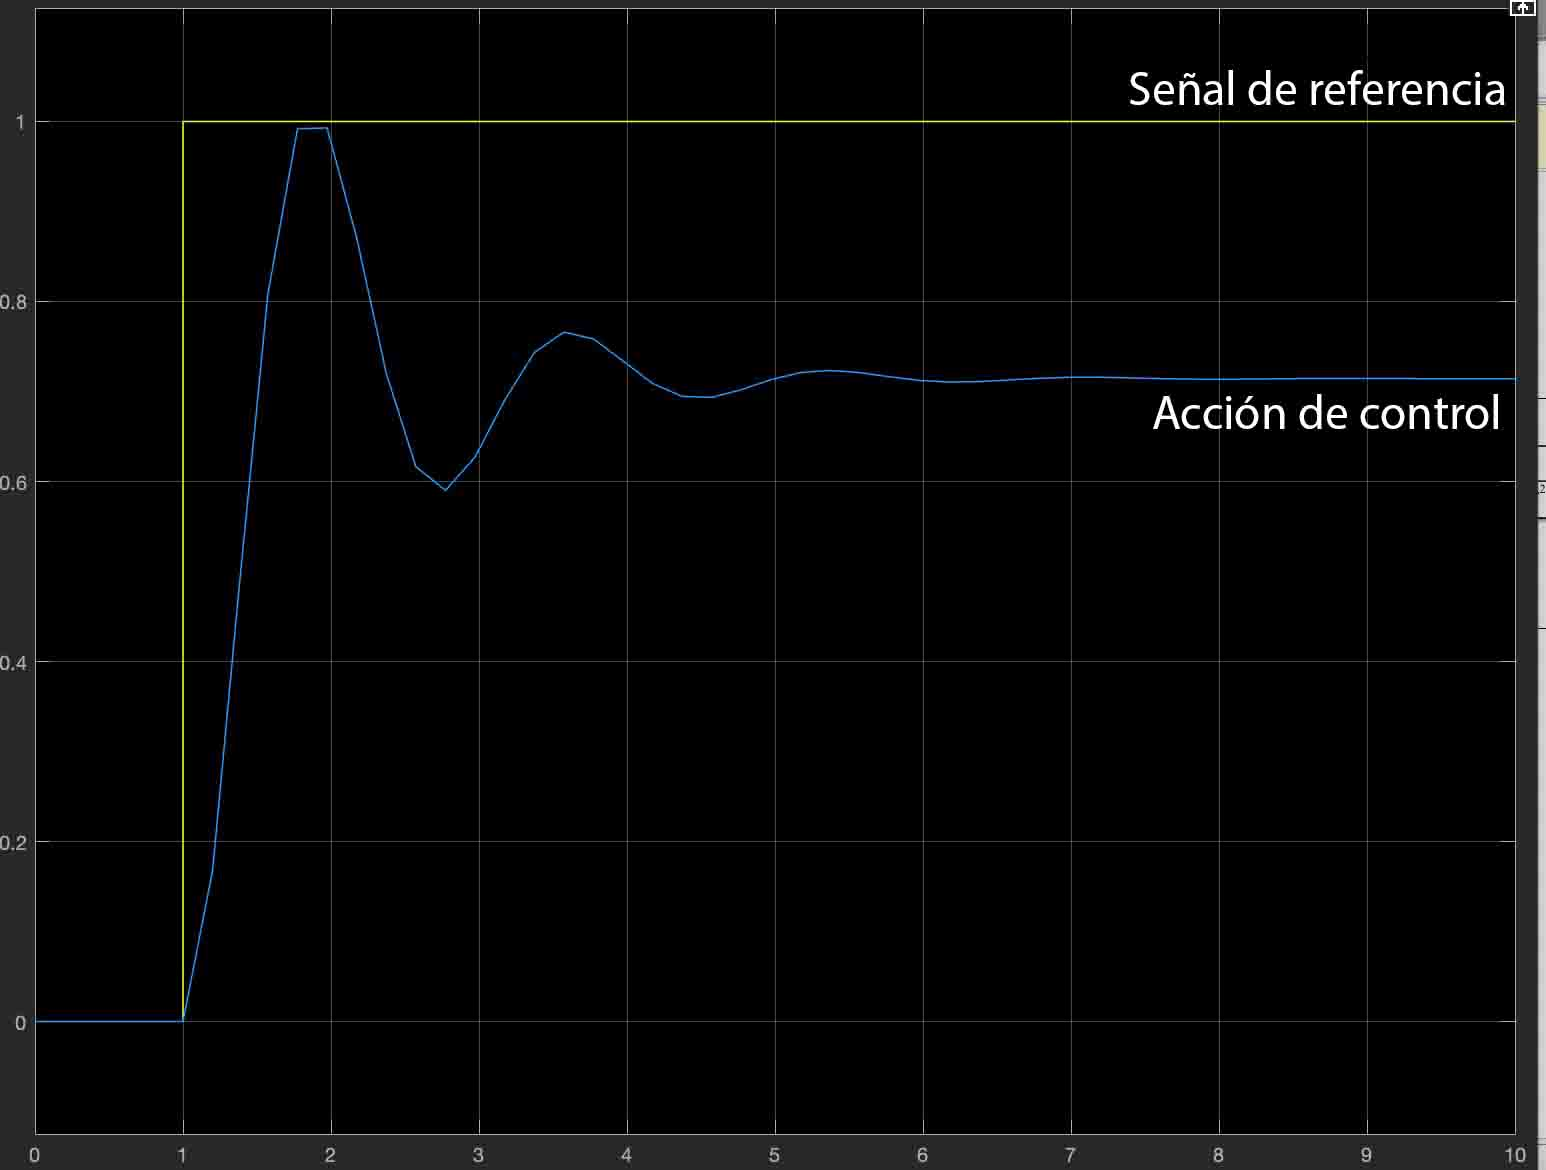
\includegraphics[width=0.7\linewidth]{MPPT/Imagen 15-10-23 a las 14.52.JPG}
    \caption{Respuesta de un control proporcional.}
    \label{fig:proporcional}
\end{figure}

La parte integral del control actua cuando hay una desviación entre la variable y el punto de consigna, integrando esta desviación en el tiempo. El error es integrado, lo cual tiene la función de promediarlo o sumarlo por un período determinado, y luego se multiplica por una constante $K_{i}$. Elimina el error de estado estacionario, logrando seguimiento perfecto de la señal de referencia. La fórmula matemática que responde a esto es:\\

\begin{equation}
    I_{sal} = K_{i} \int e(t) dt
\end{equation}


\begin{figure}[H]
    \centering
    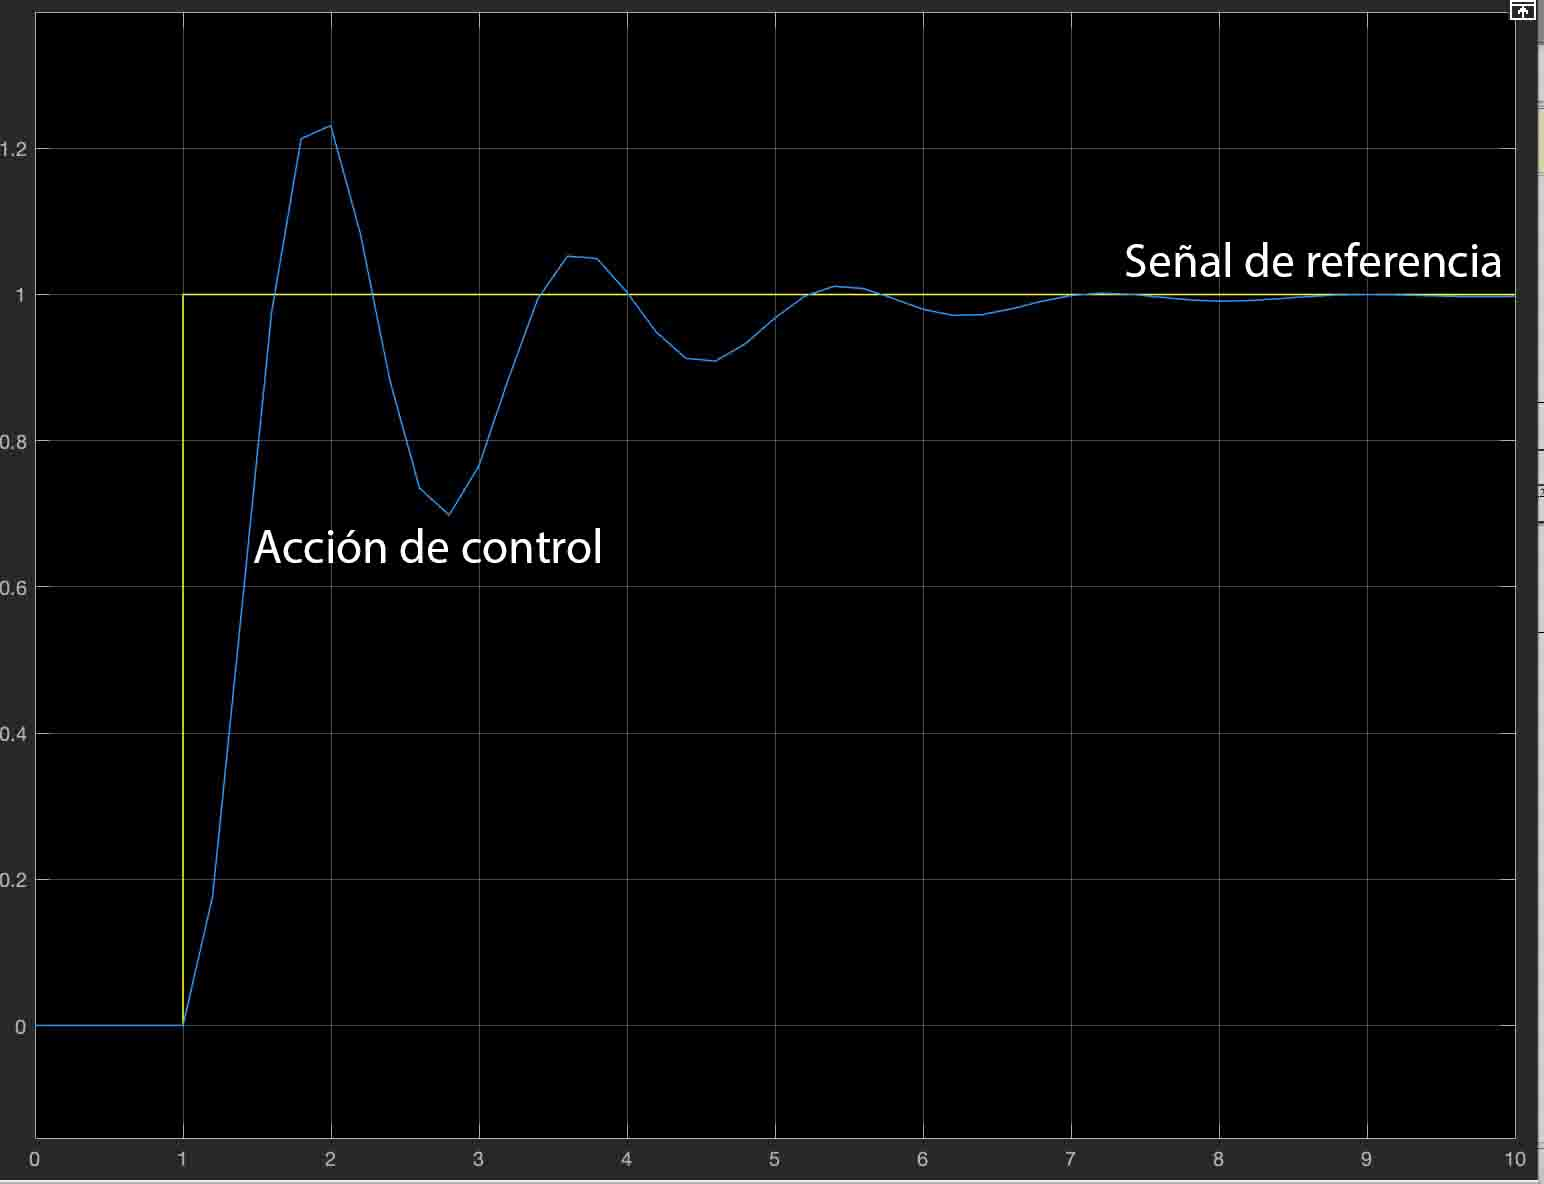
\includegraphics[width=0.7\linewidth]{MPPT/Imagen 15-10-23 a las 14.53.JPG}
    \caption{Respuesta de un control integral.}
    \label{fig:integral}
\end{figure}

Como tenemos 3 etapas de carga, donde en una la corriente es constante, y en las otras dos el voltaje lo es, vamos a necesitar controlar esas dos variables.\\

En la etapa bulk, se tendrá en cuenta el parámetro de corriente de salida y se controlará para mantenerla en un valor constante estipulado por el fabricante de la batería. En esta etapa, el voltaje será una consecuencia, y simplemente se monitorea que su valor sea menor a la tension de absorción. Si llega a este valor (tensión de absorcion), se termina la etapa bulk, y comienza la de absorción.\\

En la etapa de absorción, al contrario que la anterior, se controlará el voltaje de salida, dejando la corriente como una consecuencia. El valor de la corriente irá disminuyendo, hasta llegar a un mínimo llamado corriente de flote, donde comenzará la etapa de flote.\\

En la etapa de flote, se sigue controlando el voltaje, en este caso menor, y la corriente sigue siendo una consecuencia. En este estado se considera que la batería ya esta cargada.\\

Si la corriente de carga comienza a aumentar, es porque la batería se está utilizando, y por lo tanto está siendo descargada. Ahí es cuando se reinicia el ciclo, y empieza a correr de nuevo la etapa bulk.\\

\subsection{Realización}

\subsubsection{Hardware}

\begin{figure}[H]
    \centering
    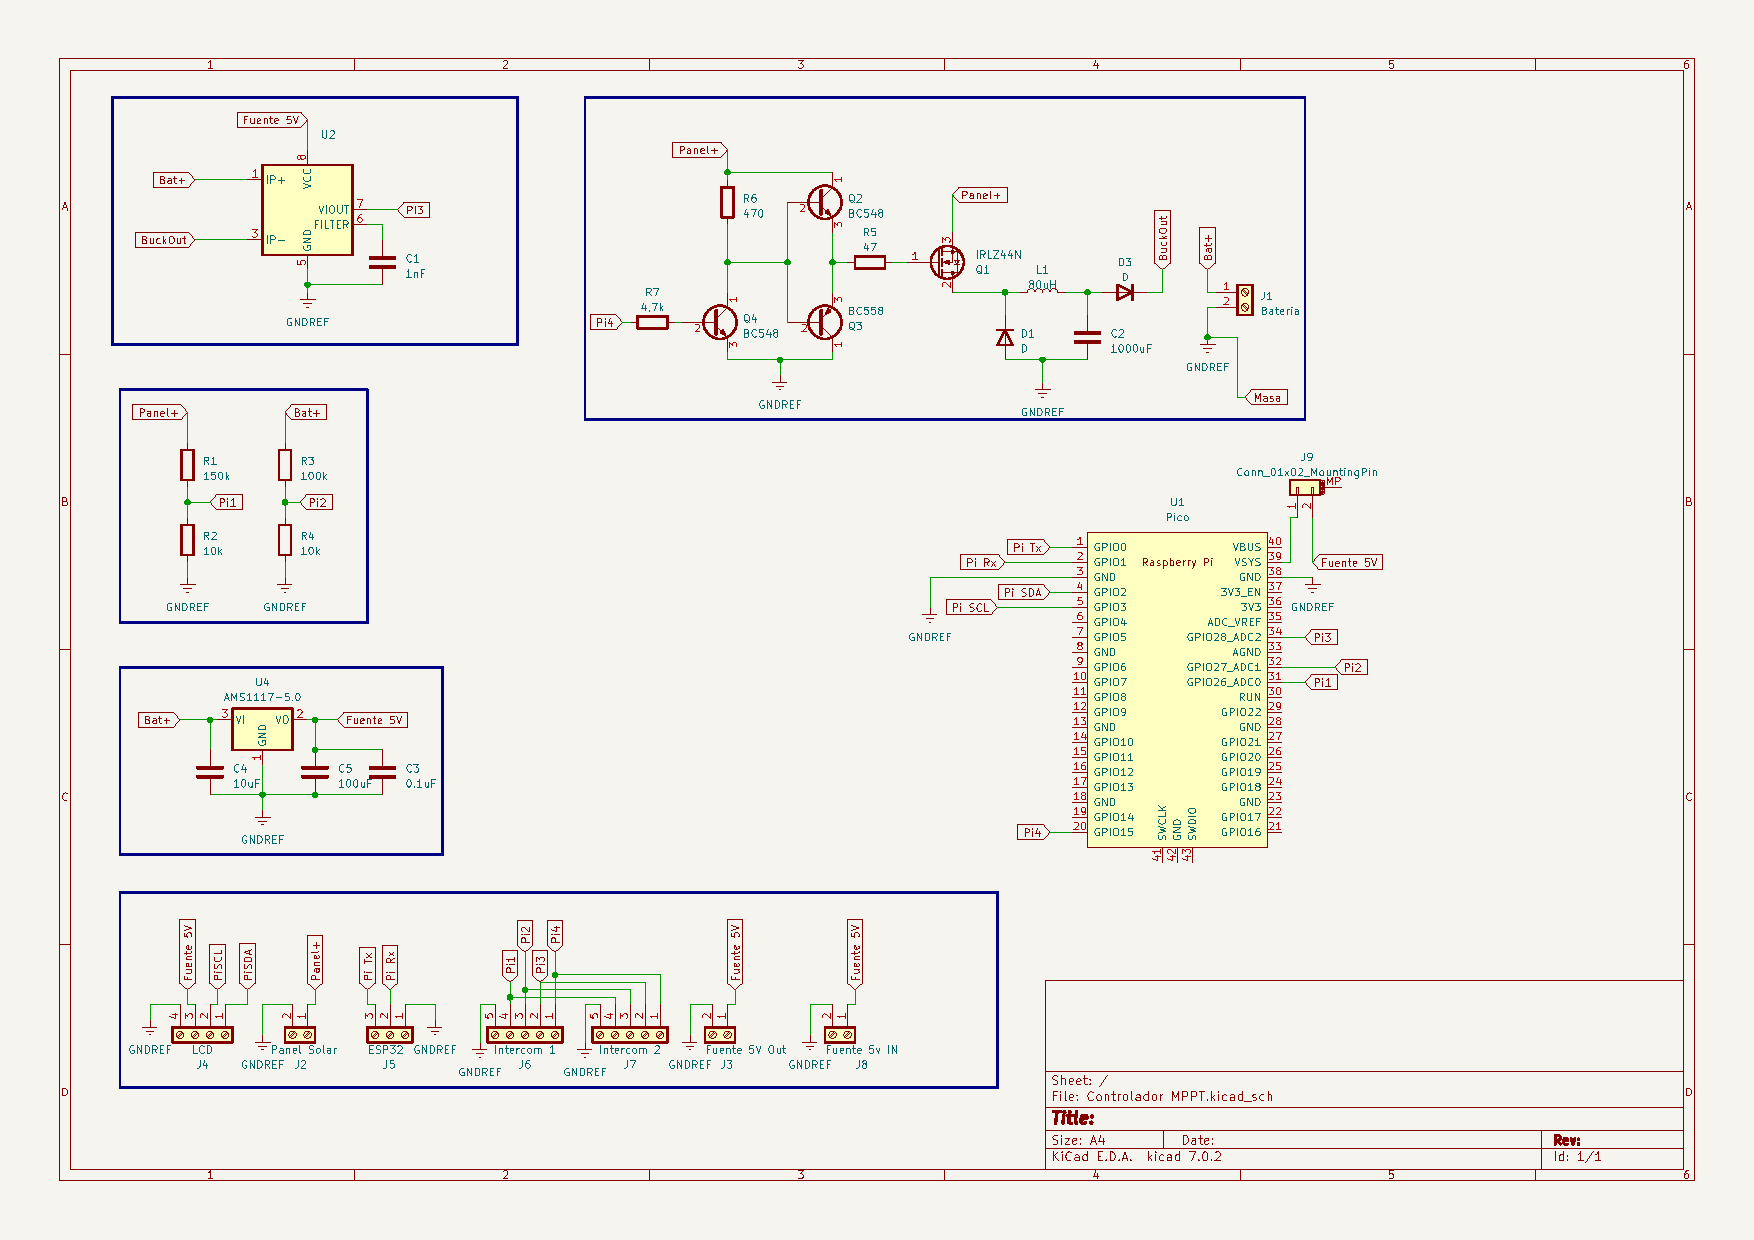
\includegraphics[width=1\linewidth]{MPPT/Controlador MPPT.pdf}
    \caption{Circuito MPPT completo.}
    \label{fig:enter-label}
\end{figure}

\begin{wrapfigure}{l}{0.35\textwidth}
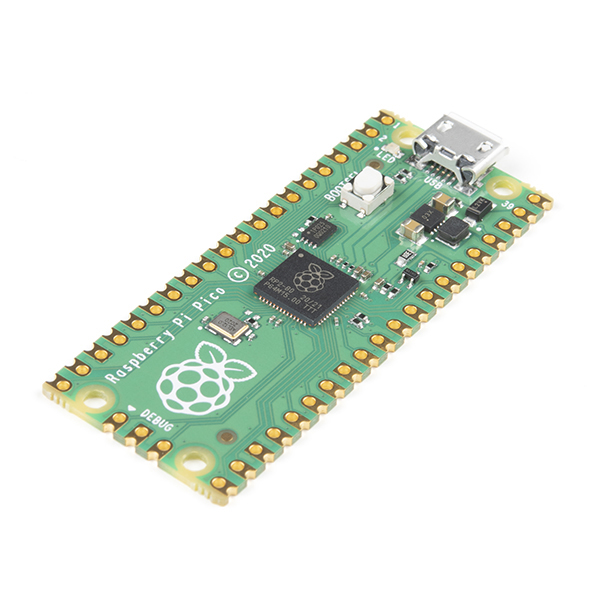
\includegraphics[width=0.9\linewidth]{MPPT/17829-Raspberry_Pi_Pico-01.jpg} 
\caption{Raspberry Pi Pico}
\label{fig:wrapfig}
\end{wrapfigure}

Para realizar este cargador, utilizamos una Raspberry Pi Pico como controlador principal, encargada de leer todos los parámetros, controlar el voltaje o la corriente de salida, y comunicarse con el módulo Solar Link para informar los parámetros medidos.\\

\begin{wrapfigure}{r}{0.25\textwidth}
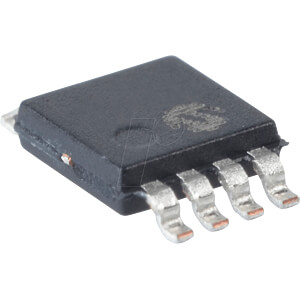
\includegraphics[width=0.9\linewidth]{MPPT/acs712.jpg} 
\caption{Sensor de corriente ACS712}
\label{fig:wrapfig}
\end{wrapfigure}

Para medir la corriente utilizamos el sensor ACS712xLCTR-20A, el cual es un sensor de efecto Hall que nos permite medir corrientes positivas y negativas, y nos devuelve esta información entre 0V y 5V. Esto quiere decir que -20A son 0V, 0A son 2,5V, y 20A son 5V. Esta información es procesada por un ADC de la Raspberry Pi Pico.\\

Para medir las tensiones tanto de entrada como de salida simplemente utilizamos divisores resistivos, los cuales nos devuelven voltajes proporcionales reducidos, tambien procesados por los otros dos ADCs de la Raspberry Pi Pico. Para la conversion simplemente se tiene en cuenta la relacion de las resistencias.\\

Para la alimentación del circuito aprovechamos el voltaje de entrada de la batería, donde conectamos una fuente Step Down que regula el voltaje de alimentacion de la Raspberry Pi Pico en 5V. Esto quiere decir que una vez que se conecta la batería para comenzar la carga, el circuito ya se encuentra alimentado por energía verde para funcionar.\\

Para mostrar los datos medidos en tiempo real, utilizamos un LCD de 20x04, donde entran se pueden mostrar sin problemas estos datos. El cargador indica el voltaje de entrada, voltaje de salida, corriente de salida, \% de PWM utilizado, y fase de carga.\\

\begin{figure}[H]
    \centering
    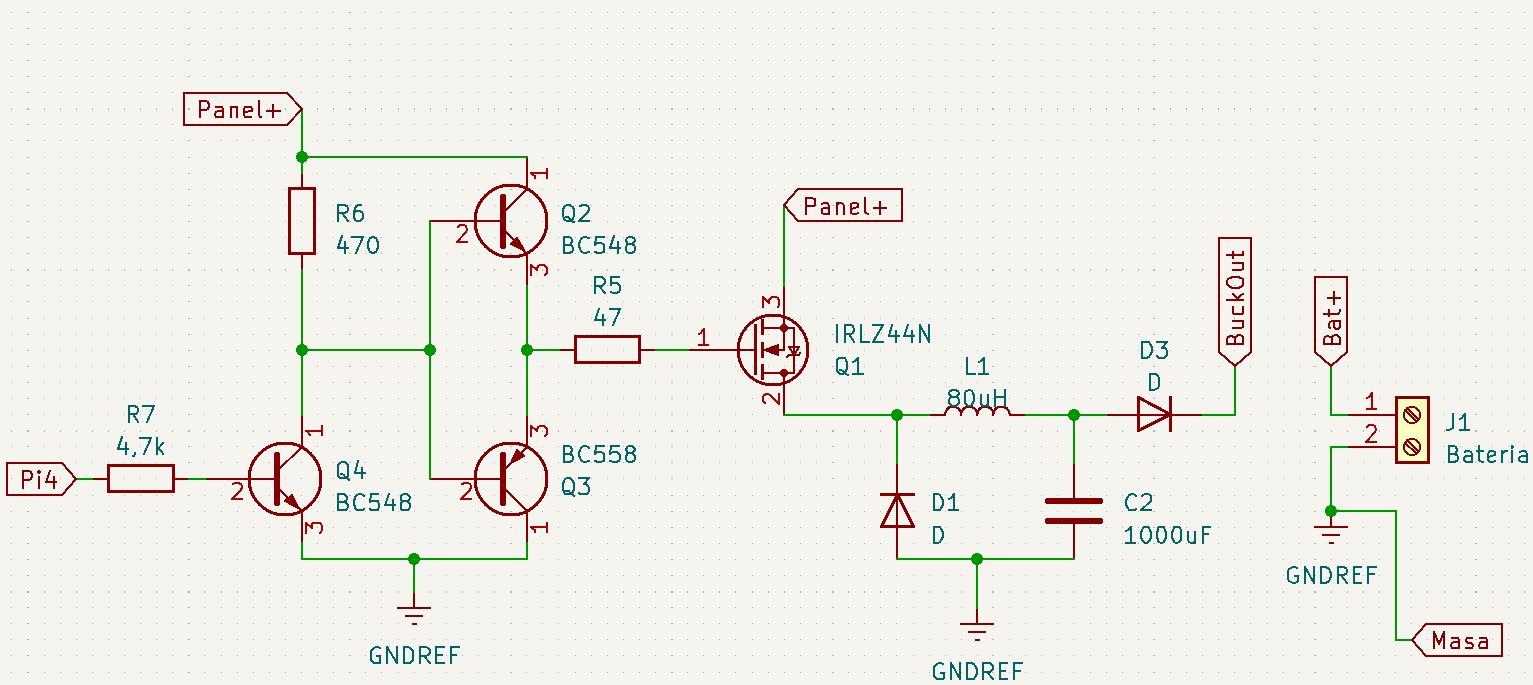
\includegraphics[width=1\linewidth]{MPPT/Screenshot_7.png}
    \caption{Circuito MPPT.}
    \label{fig:circuito MPPT}
\end{figure}

En el circuito MPPT, la única diferencia con el teórico es el interruptor. Nuestro interruptor es un MOSFET canal P \href{https://www.alldatasheet.es/datasheet-pdf/pdf/683453/KERSEMI/IRF4905.html}{IRF4905}, que resiste hasta 70A de corriente. Es necesaria la utilización de un MOSFET canal P porque la carga del mismo tiene que estar entre Drain y Masa, mientras que la carga de un canal N tiene que estar entre la alimentación y Source, algo que en nuestro diseño resultó inconveniente.\\

Para conmutar este MOSFET con la Raspberry Pi Pico, no solo fue necesaria la utilización de un transistor NPN, sino tambien la de un circuito totem pole. \\

\begin{figure}[H]
    \centering
    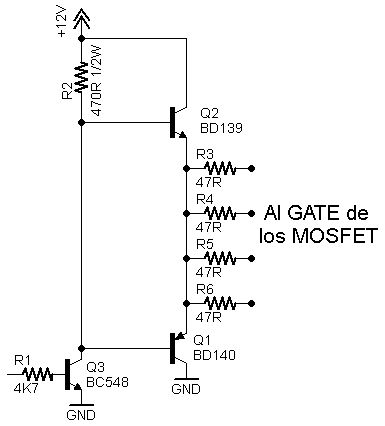
\includegraphics[width=0.8\linewidth]{MPPT/Imagen de WhatsApp 2023-10-11 a las 20.57.02_7faa2d47.jpg}
    \caption{Circuito Totem Pole.}
    \label{fig:enter-label}
\end{figure}

Un circuito totem pole consta de 2 transistores, un PNP y un NPN, uno arriba del otro, con sus bases interconectadas. Esto nos permite conmutar el MOSFET sin problemas, porque admite corrientes en ambos sentidos, tanto positivas como negativas. Esto es necesario porque un MOSFET necesita ambos sentidos de corrientes. Para entrar en estado de corte, necesita una corriente positiva en el Gate, y para volver al estado de saturación, por las características capacitivas del mismo, genera una corriente negativa.\\

Para el cálculo del inductor, se realizó el siguiente procedimiento:

Fijándose en la figura \ref{fig:grafica-mppt}, el aumento de la corriente en la bobina queda:

\begin{equation}
\frac{di_L(t)}{dt} = \frac{V_L(t)}{L} = \frac{V_i - V_o}{L}    
\end{equation}

y análogamente el descenso de corriente es:

\begin{equation}
\frac{di_L(t)}{dt} = \frac{V_L(t)}{L} = \frac{-V_o}{L}    
\end{equation}

Como toda la energía que se almacena en la bobina durante el primer estado se transfiere durante el segundo, la energía del inductor al final del periodo de conmutación ($T_S$) es igual en $t = 0$ y en $t = T_S$.\\

Por lo tanto, la tensión media en la bobina $\langle V_L \rangle$ en régimen permanente es nula, es decir, existe una igualdad en las áreas.

\begin{equation}
    \langle V_L \rangle = \frac{1}{T_s}\int_{T_s} V_L dt = 0
\end{equation}

Aplicando la ecuación se obtiene:

\begin{equation}
    (V_i - V_o) \cdot DT_s - V_o \cdot (T_s - DT_s) = 0
\end{equation}

Donde D es un número adimensional, entre 0 y 1, denominado ciclo de trabajo. Siendo que este no puede ser mayor a 1, se cumple $V_o \leq V_i$, por tanto solo se podrá reducir la tensión.

\begin{equation}
    V_o = D \cdot V_i
    \label{eq:D}
\end{equation}

La corriente media que circula por la bobina, con un D del 10\% (peor condición posible):\\

\begin{equation}
    I_L > \frac{I_{Lmax}}{10} = 2
\end{equation}



\begin{equation}
    \frac{\Delta I_L}{2} < 2 \Rightarrow \Delta I_L < 4
\end{equation}\\

Para calcular la bobina, se utiliza la siguiente fórmula:\\

\begin{equation}
    \frac{V_i - V_o}{L} \cdot D \cdot T_S < 4
\end{equation}\\

Reemplazando D por la equivalencia obtenida en la fórmula \ref{eq:D}, queda:\\

\begin{equation}
    L \geq \frac{V_o(1-\frac{V_o}{V_i})\cdot T_S}{4}
\end{equation}

Siendo
\[V_i [12V-36V]\]
\[V_o [12V-15V]\]
\[T_S = 32 \cdot 10^{-6} S  = 32KHz\]\\

El máximo de esta función queda definido por los máximos valores de tensión de entrada y tensión de salida, por lo tanto:\\

\begin{equation}
    L \geq \frac{15 \cdot (1-\frac{15}{36}) \cdot 32 \cdot 10^{-6}}{4}
\end{equation}

Entonces \[L \geq 68uH\]\\

La bobina utilizada en el circuito posee un valor de \textbf{$83uH$}, la cual cumple con la condición anterior.\\

Para el cálculo del capacitor correspondiente, se realizó el siguiente procedimiento:\\

Cálculo para el ripple del capacitor de un 1\%: 

\begin{equation}
    \Delta V_o = 1\% \cdot 15V = 0,15V
\end{equation}

La fórmula utilizada para obtener el valor del capacitor es la siguiente:\\

\begin{equation}
    \Delta V_o = \frac{V_o \cdot (1-\frac{V_o}{V_i})}{8 \cdot L \cdot C \cdot F^2}
\end{equation}\\

Despejando, se obtiene:\\

\begin{equation}
    C \geq \frac{V_o \cdot  (1 - \frac{V_o}{V_i})}{8 \cdot L \cdot \Delta V_o \cdot F^2}
\end{equation}\\

Con los valores ya calculados, se reemplazan los parámetros:\\

\begin{equation}
    C \geq \frac{15V \cdot (1 - \frac{15V}{36V})}{8 \cdot 83uH \cdot 32KHz^2}
\end{equation}

Entonces \[C \geq 12uF\]\\

Para evitar resonancias, se estima que la frecuencia de resonancia tiene que estar 10 veces por debajo de la frecuencia en la que se trabaja. Por esto:\\

\begin{equation}
    \frac{F_S}{10} = \frac{1}{\sqrt{L \cdot C}}
\end{equation}

Despejando, queda:\\

\begin{equation}
    C = \frac{10^2}{32KHz^2 \cdot 83uH} \simeq 1100uF
\end{equation}\\

Por lo tanto, en el circuito final se utilizó un capacitor de \textbf{$1000uF$}

\subsubsection{Software}

El sistema MPPT fue programado íntegramente con el lenguaje C sobre la Raspberry Pi Pico. \\

El microcontrolador lee las señales del divisor de tensión que caerá sobre sus ADC y, mediante una lógica dependiente de la relación entre las resistencias del divisor de tensión, el código interpreta estas señales para saber el valor deseado (ya sea corriente o votaje). Referirse a Listing \ref{Listing 1}  o Listing \ref{Listing 2}\\

Ya sabiendo los valores que se tienen que medir, se compararán con los valores definidos para el cambio de lógica. Así se define en que modo de carga estará el MPPT. Por ejemplo, para el cambio entre BULK y ABSORTION, el voltaje de la batería deberá ser mayor al voltaje máximo definido del modo BULK. Referirse a Listing \ref{Listing 3}, pag 25\\

Tambien, cada vez que se define el modo y los valores de cada variable, se los mostrara en un display LCD. \\

Cada modo tiene su propia lógica para manejar el PWM que regula la tensión y corriente que le llega a la batería. En el modo BULK, primero se calcula el error entre la medicion actual y la deseada, luego se ve si la corriente que le llega a la batería es mayor o menor a la deseada y en base a esto se controla el PWM proporcionalmente e integralmente tomando en cuenta el error (Referirse a Listing \ref{Listing 4}), pasando previamente por un saturador, asegurándose que el valor del PWM no sea ni mayor a 100\% ni menor a 0\%. Referirse a Listing \ref{Listing 5}\\

Luego de todo este proceso, el valor actual del PWM es mostrado en la pantalla del LCD. Referirse a Listing \ref{Listing 6}\\

Para la comunicación con el otro microcontrolador, se utiliza UART. Con este objetivo, la Raspberry Pi Pico realiza una interrupción cada 1 segundo, reteniendo los datos de consumo actual. Cada 60 segundos estos datos se promediarán y se guardarán en otra variable, aumentando un contador (Referirse a Listing \ref{Listing 7}). Cuando el otro micro mande una señal, se promediaran los valores guardados y se enviara un promedio de consumo. Referirse a Listing \ref{Listing 8}\\

\subsubsection{Resultado final}

El prototipo final de nuestro cargador MPPT de 3 etapas es completamente funcional, probado con paneles solares y diferentes baterías, sin presentar fallas despues de horas de funcionamiento.\\

En las pruebas realizadas, se concluyó que es un cargador muy versátil, que con cambiar unos pocos parámetros se pueden cargar todo tipo de baterías de plomo-ácido, en un tiempo razonable, y entregando una carga profunda muy saludable para la vida útil de una batería.\\

\begin{figure}[H]
    \centering
    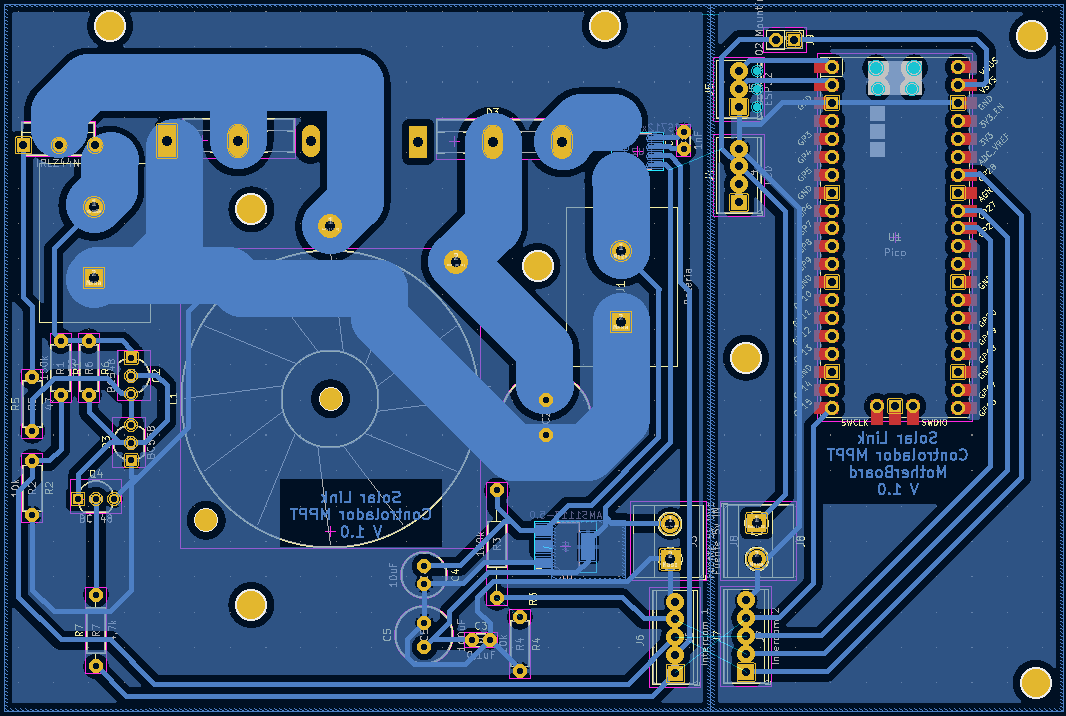
\includegraphics[width=1\linewidth]{MPPT/Screenshot_9.png}
    \caption{Diseño PCB.}
    \label{fig:PCB-MPPT}
\end{figure}

\begin{figure}[h]

\begin{subfigure}{0.5\textwidth}
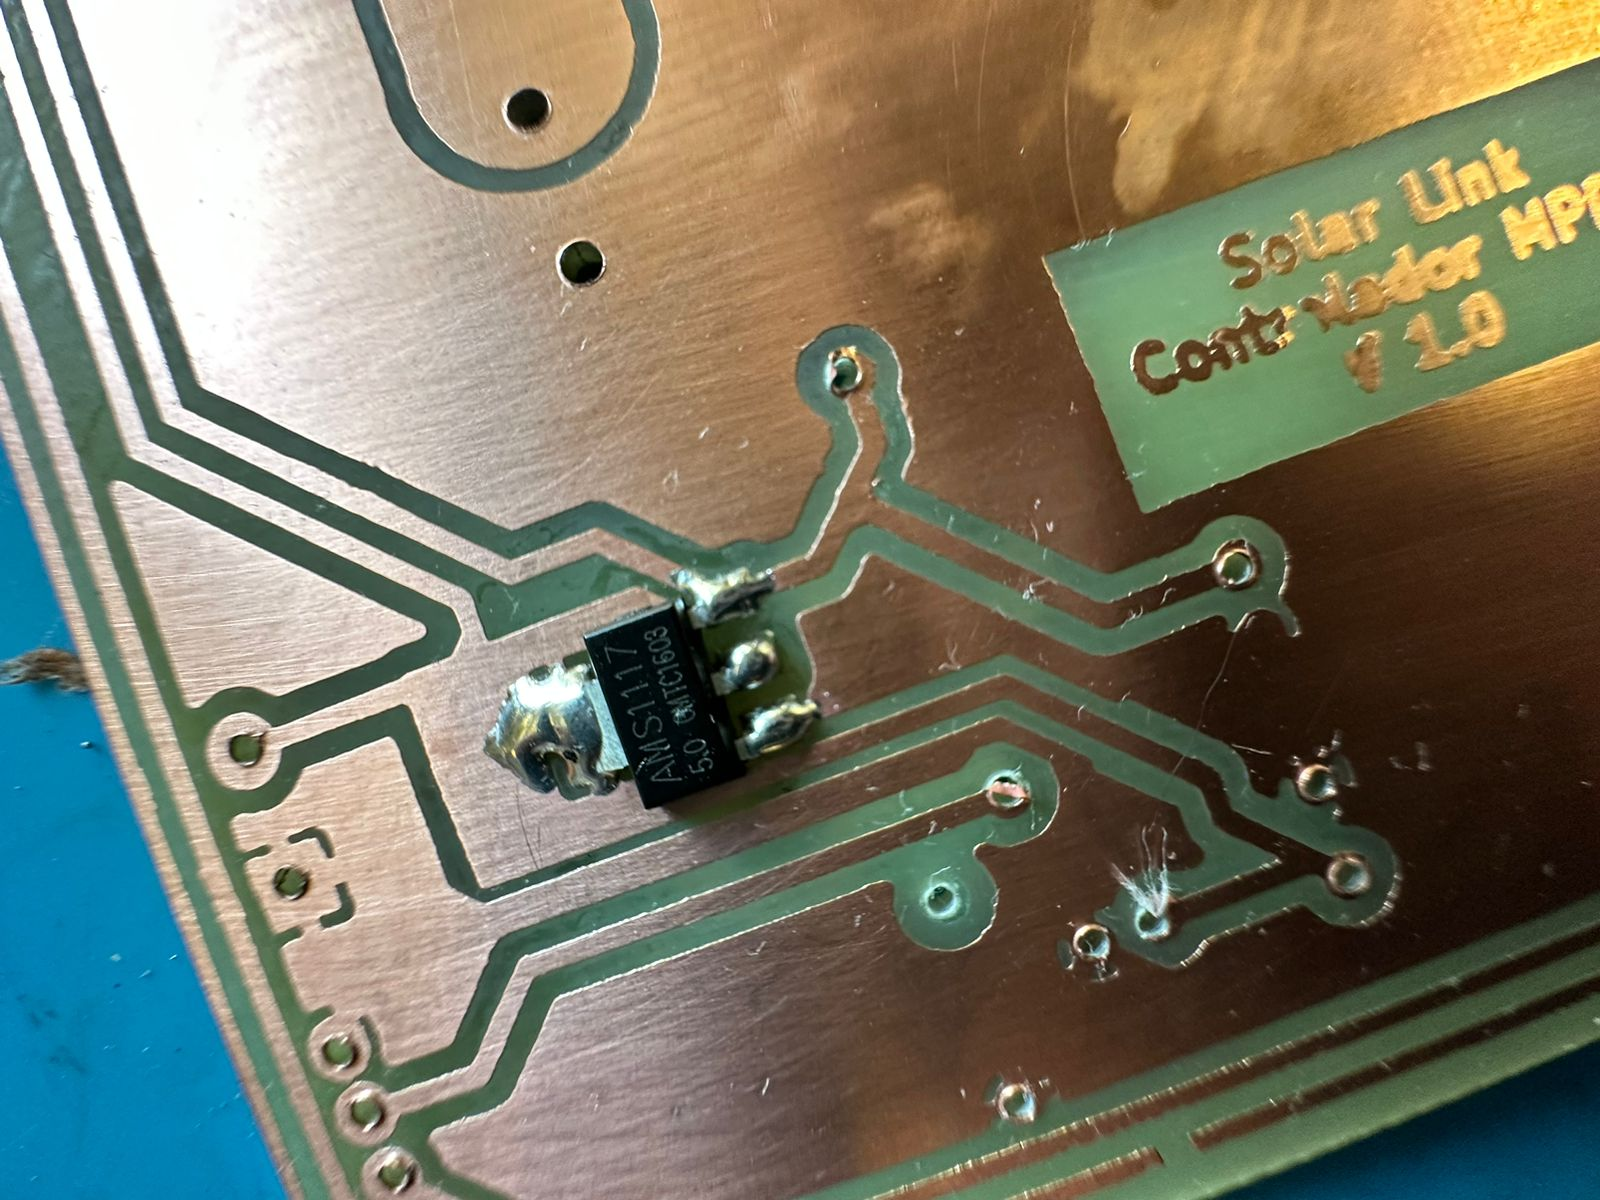
\includegraphics[width=0.9\linewidth]{MPPT/IMG_8867.JPG} 
\caption{Regulador 5V}
\label{fig:regulador12}
\end{subfigure}
\begin{subfigure}{0.5\textwidth}
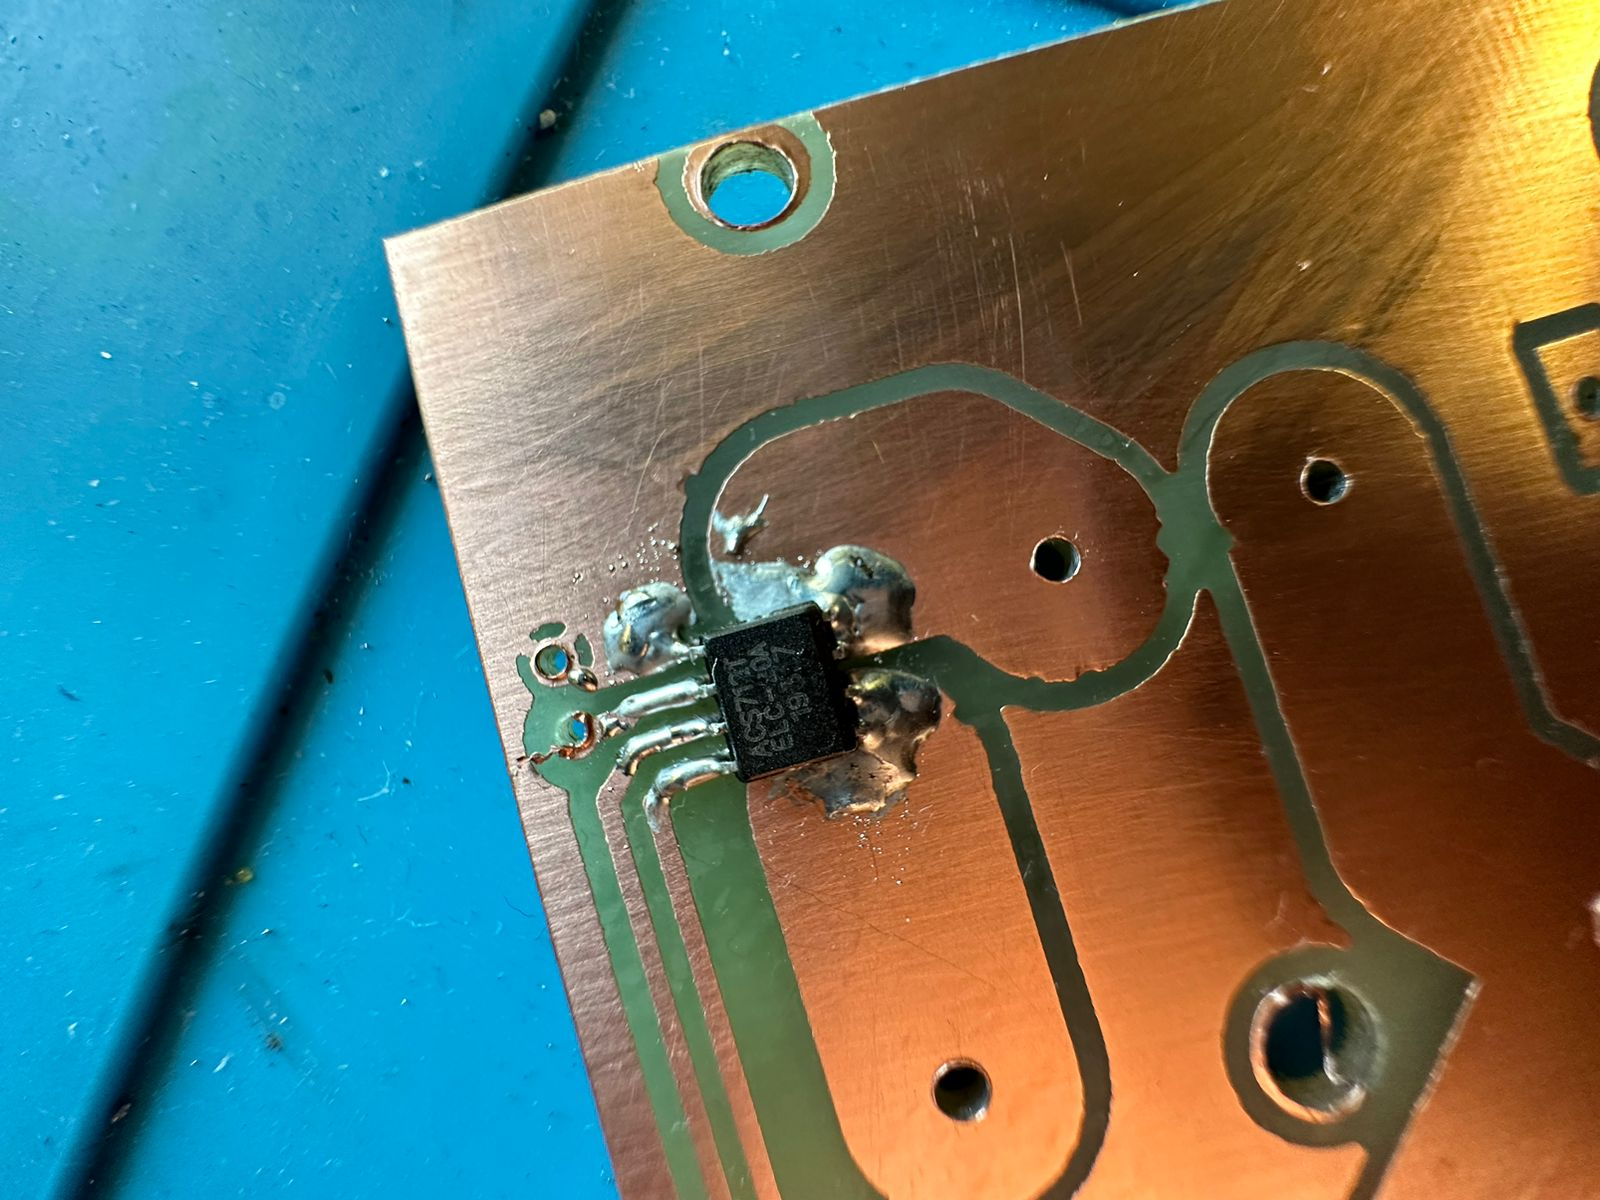
\includegraphics[width=0.9\linewidth]{MPPT/IMG_8868.JPG}
\caption{Sensor de corriente ACS712}
\label{fig:sensor-corr}
\end{subfigure}

\caption{Soladura SMD en la placa.}
\label{fig:image2}
\end{figure}

\begin{figure}[H]
    \begin{subfigure}{0.5\textwidth}
        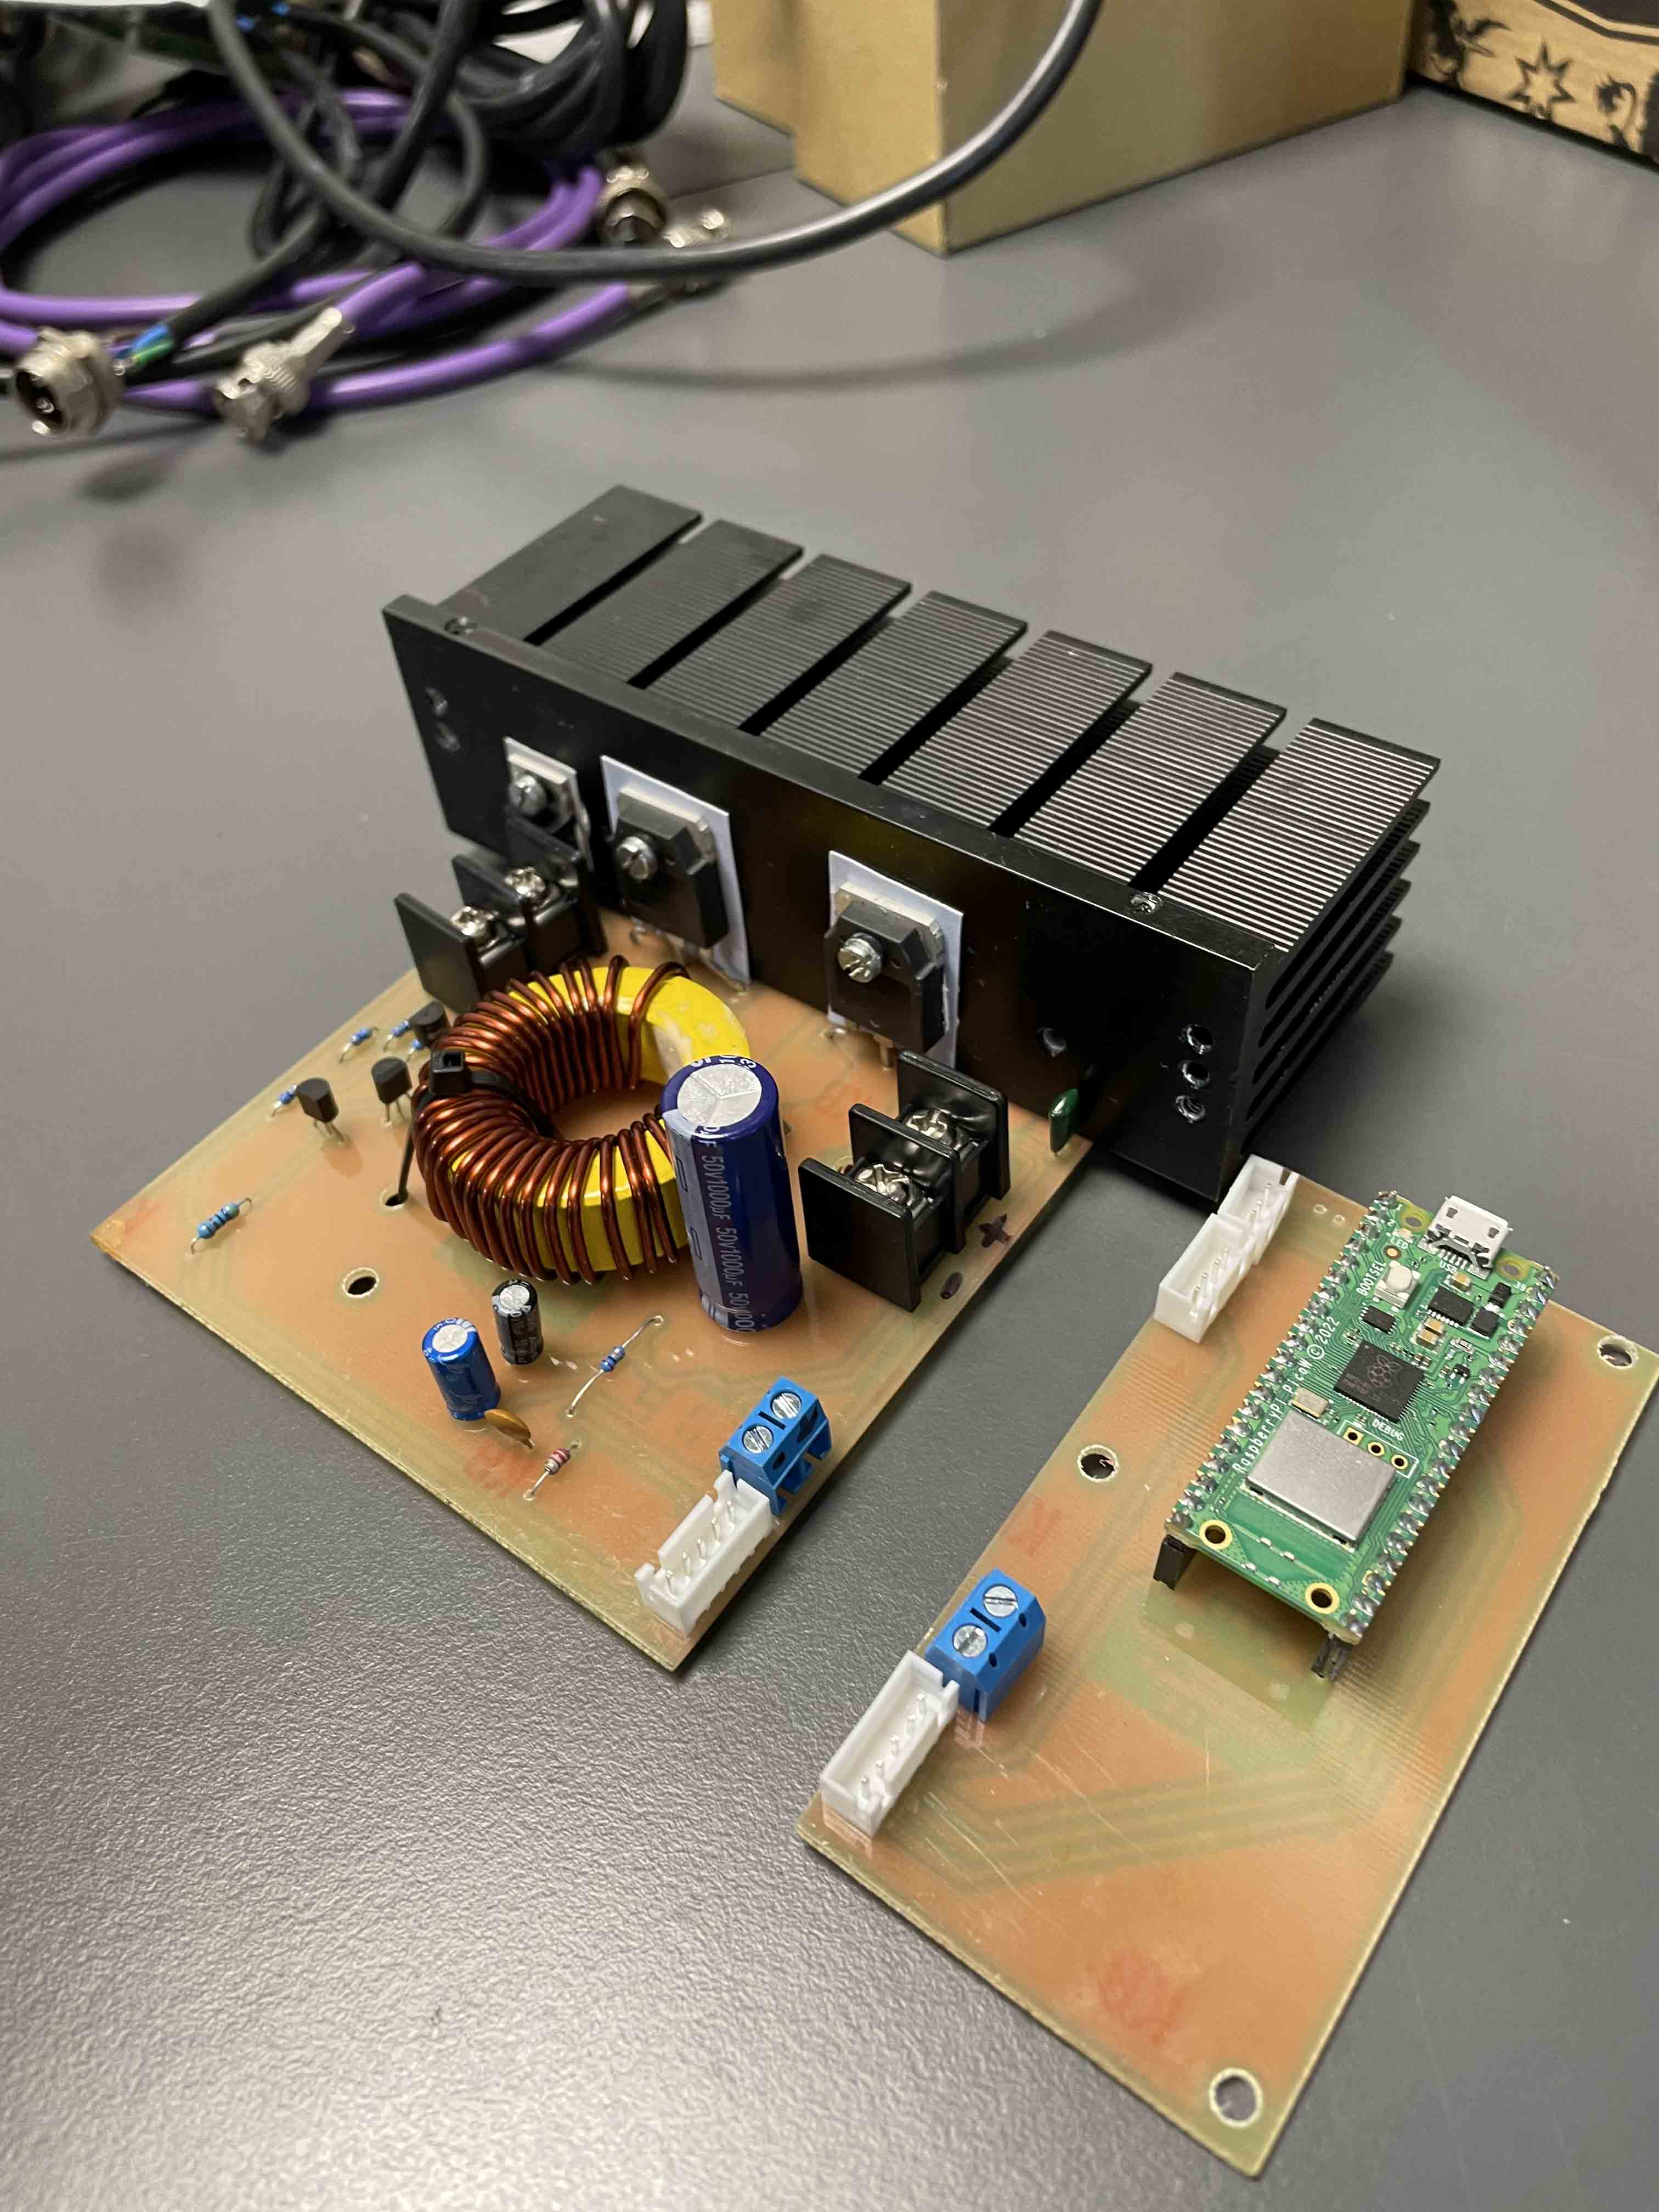
\includegraphics[width=0.9\linewidth]{MPPT/IMG_8864.jpg} 
        \caption{Plaqueta final del cargador.}
        \label{fig:subim1}
    \end{subfigure}
    \begin{subfigure}{0.5\textwidth}
        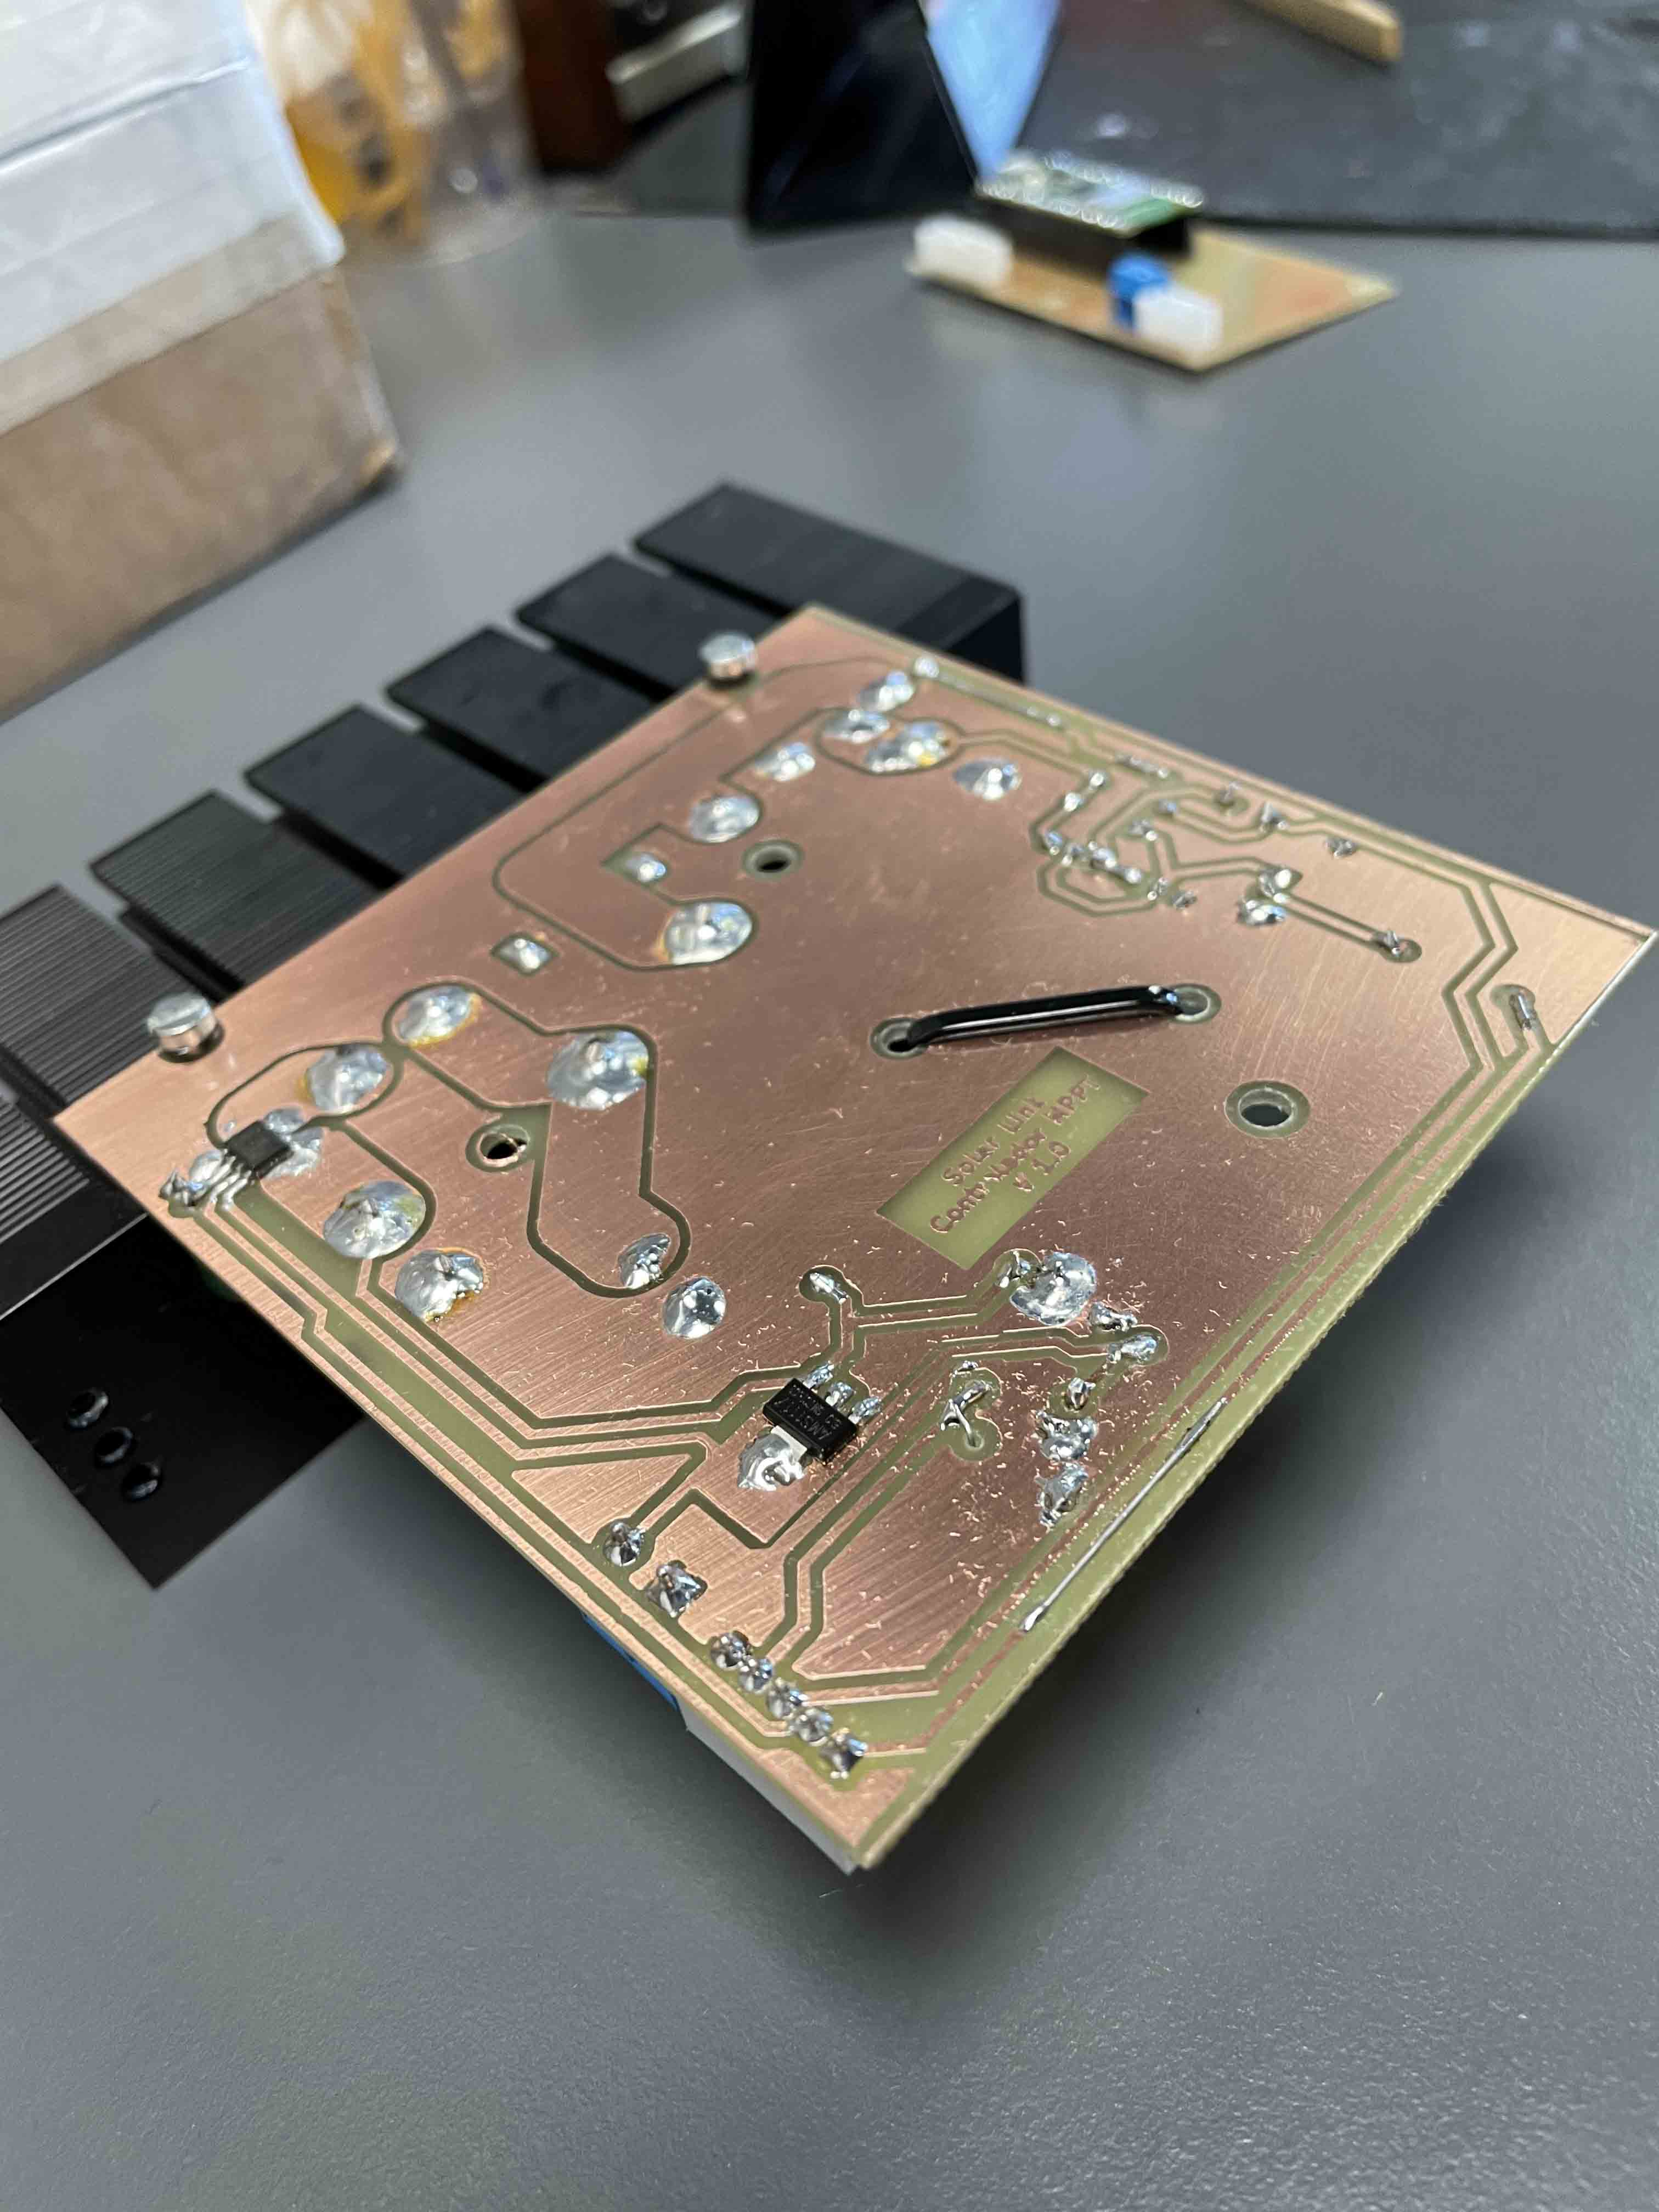
\includegraphics[width=0.9\linewidth]{MPPT/IMG_8866.jpg}
        \caption{Plaqueta final, lado inferior.}
        \label{fig:subim2}
    \end{subfigure}
\caption{Plaquetas finales cargador MPPT.}
\end{figure}

\begin{figure}[H]
    \begin{subfigure}{0.5\textwidth}
        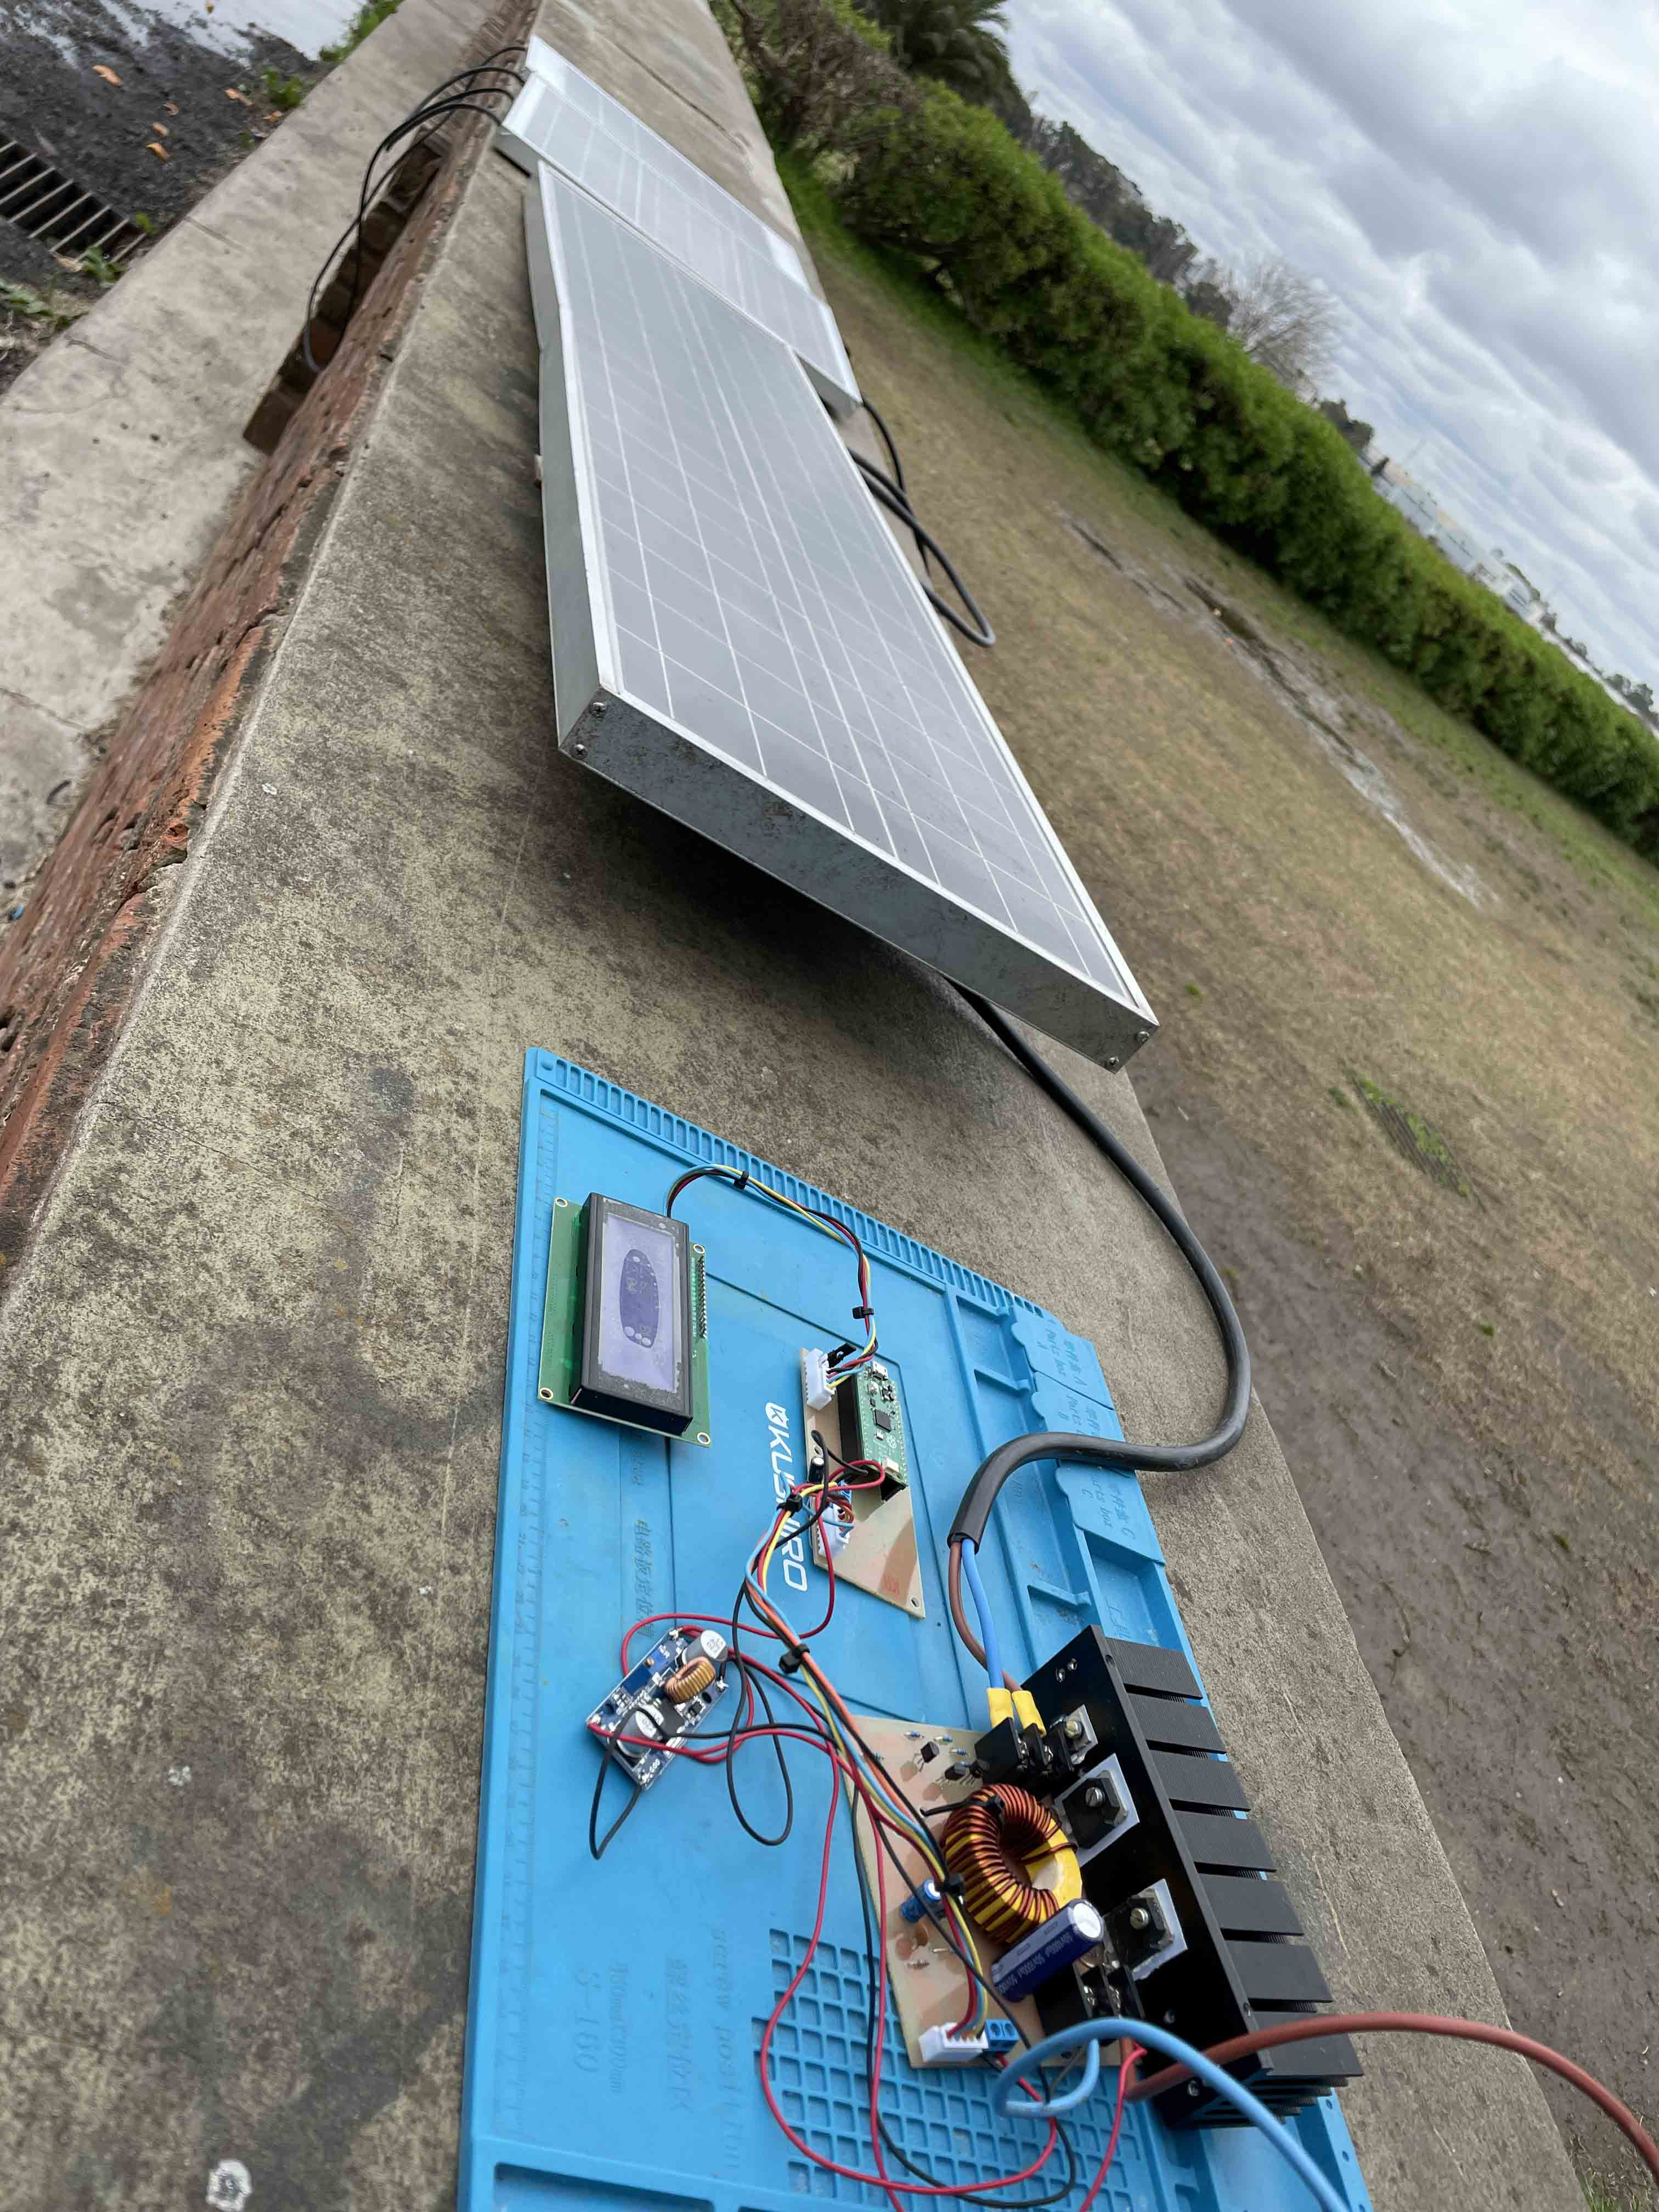
\includegraphics[width=0.9\linewidth]{MPPT/IMG_8913.jpg} 
        \caption{Cargador conectado a paneles\\ solares.}
        \label{fig:paneles-solares-MPPT}
    \end{subfigure}
    \begin{subfigure}{0.5\textwidth}
        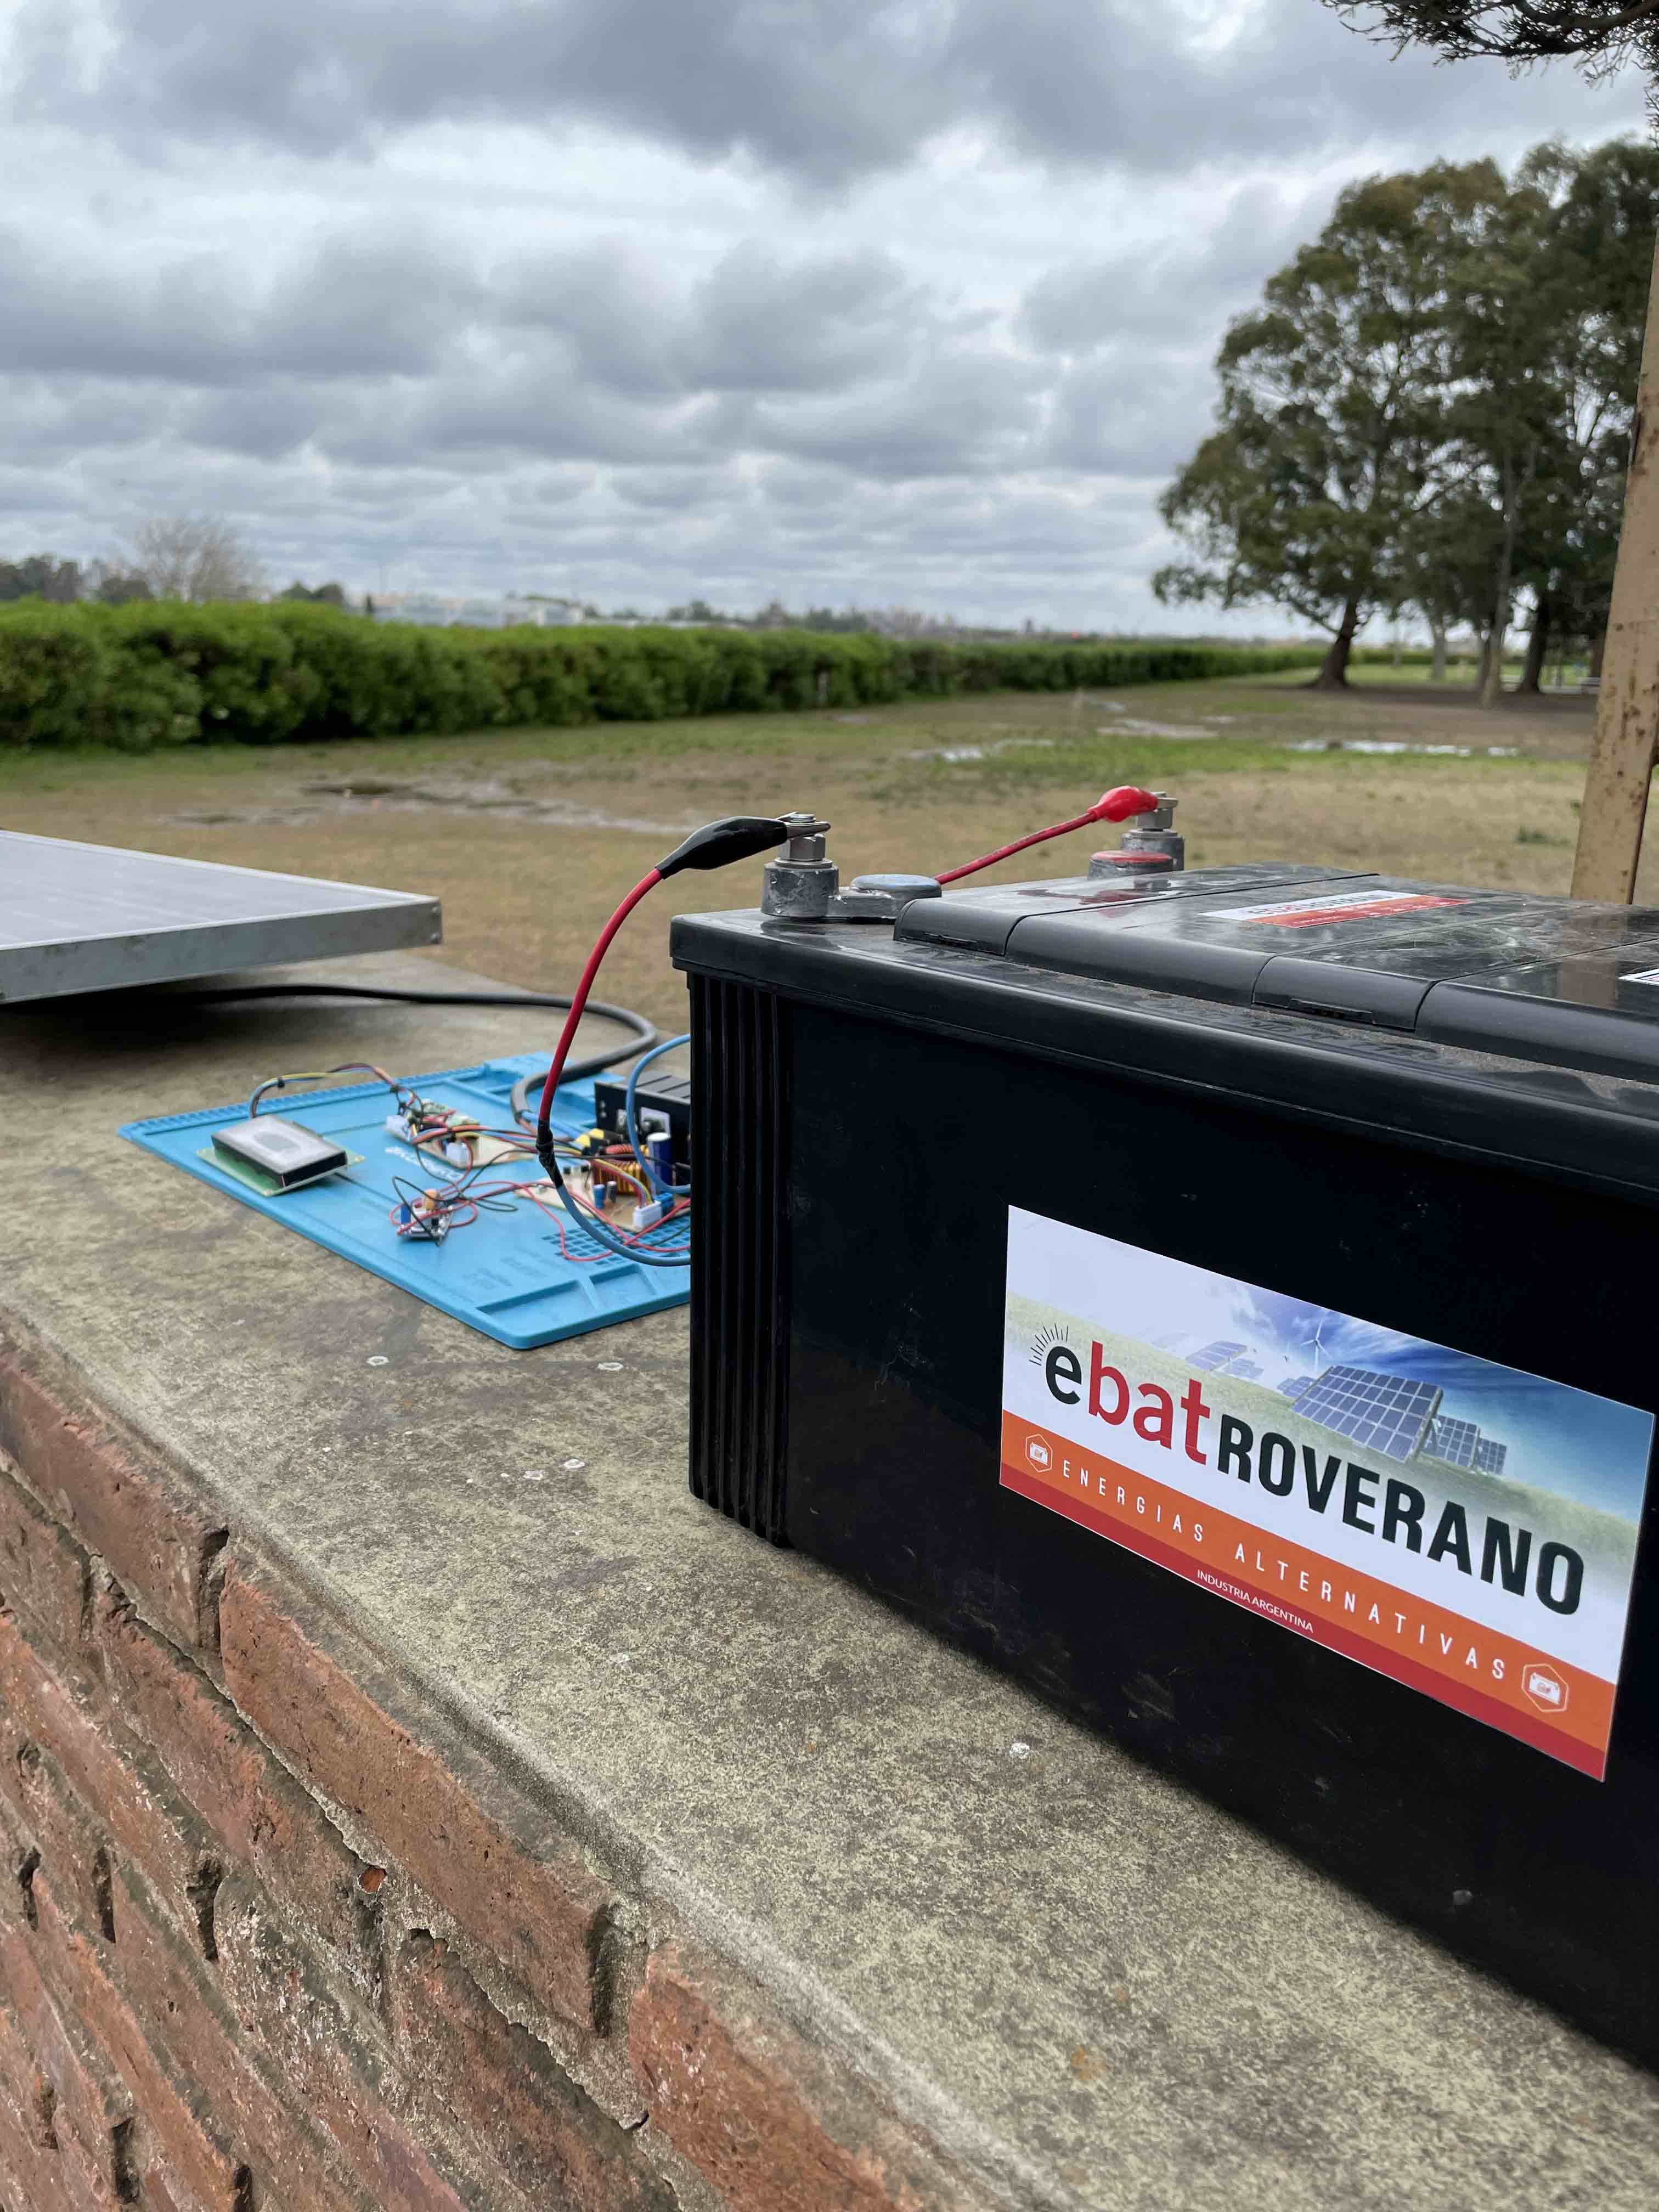
\includegraphics[width=0.9\linewidth]{MPPT/IMG_8915.jpg}
        \caption{Cargador conectado a una batería\\ de ciclo profundo.}
        \label{fig:MPPT-bateria}
    \end{subfigure}
\caption{Cargador MPPT en uso.}
\end{figure}

\begin{figure}[H]
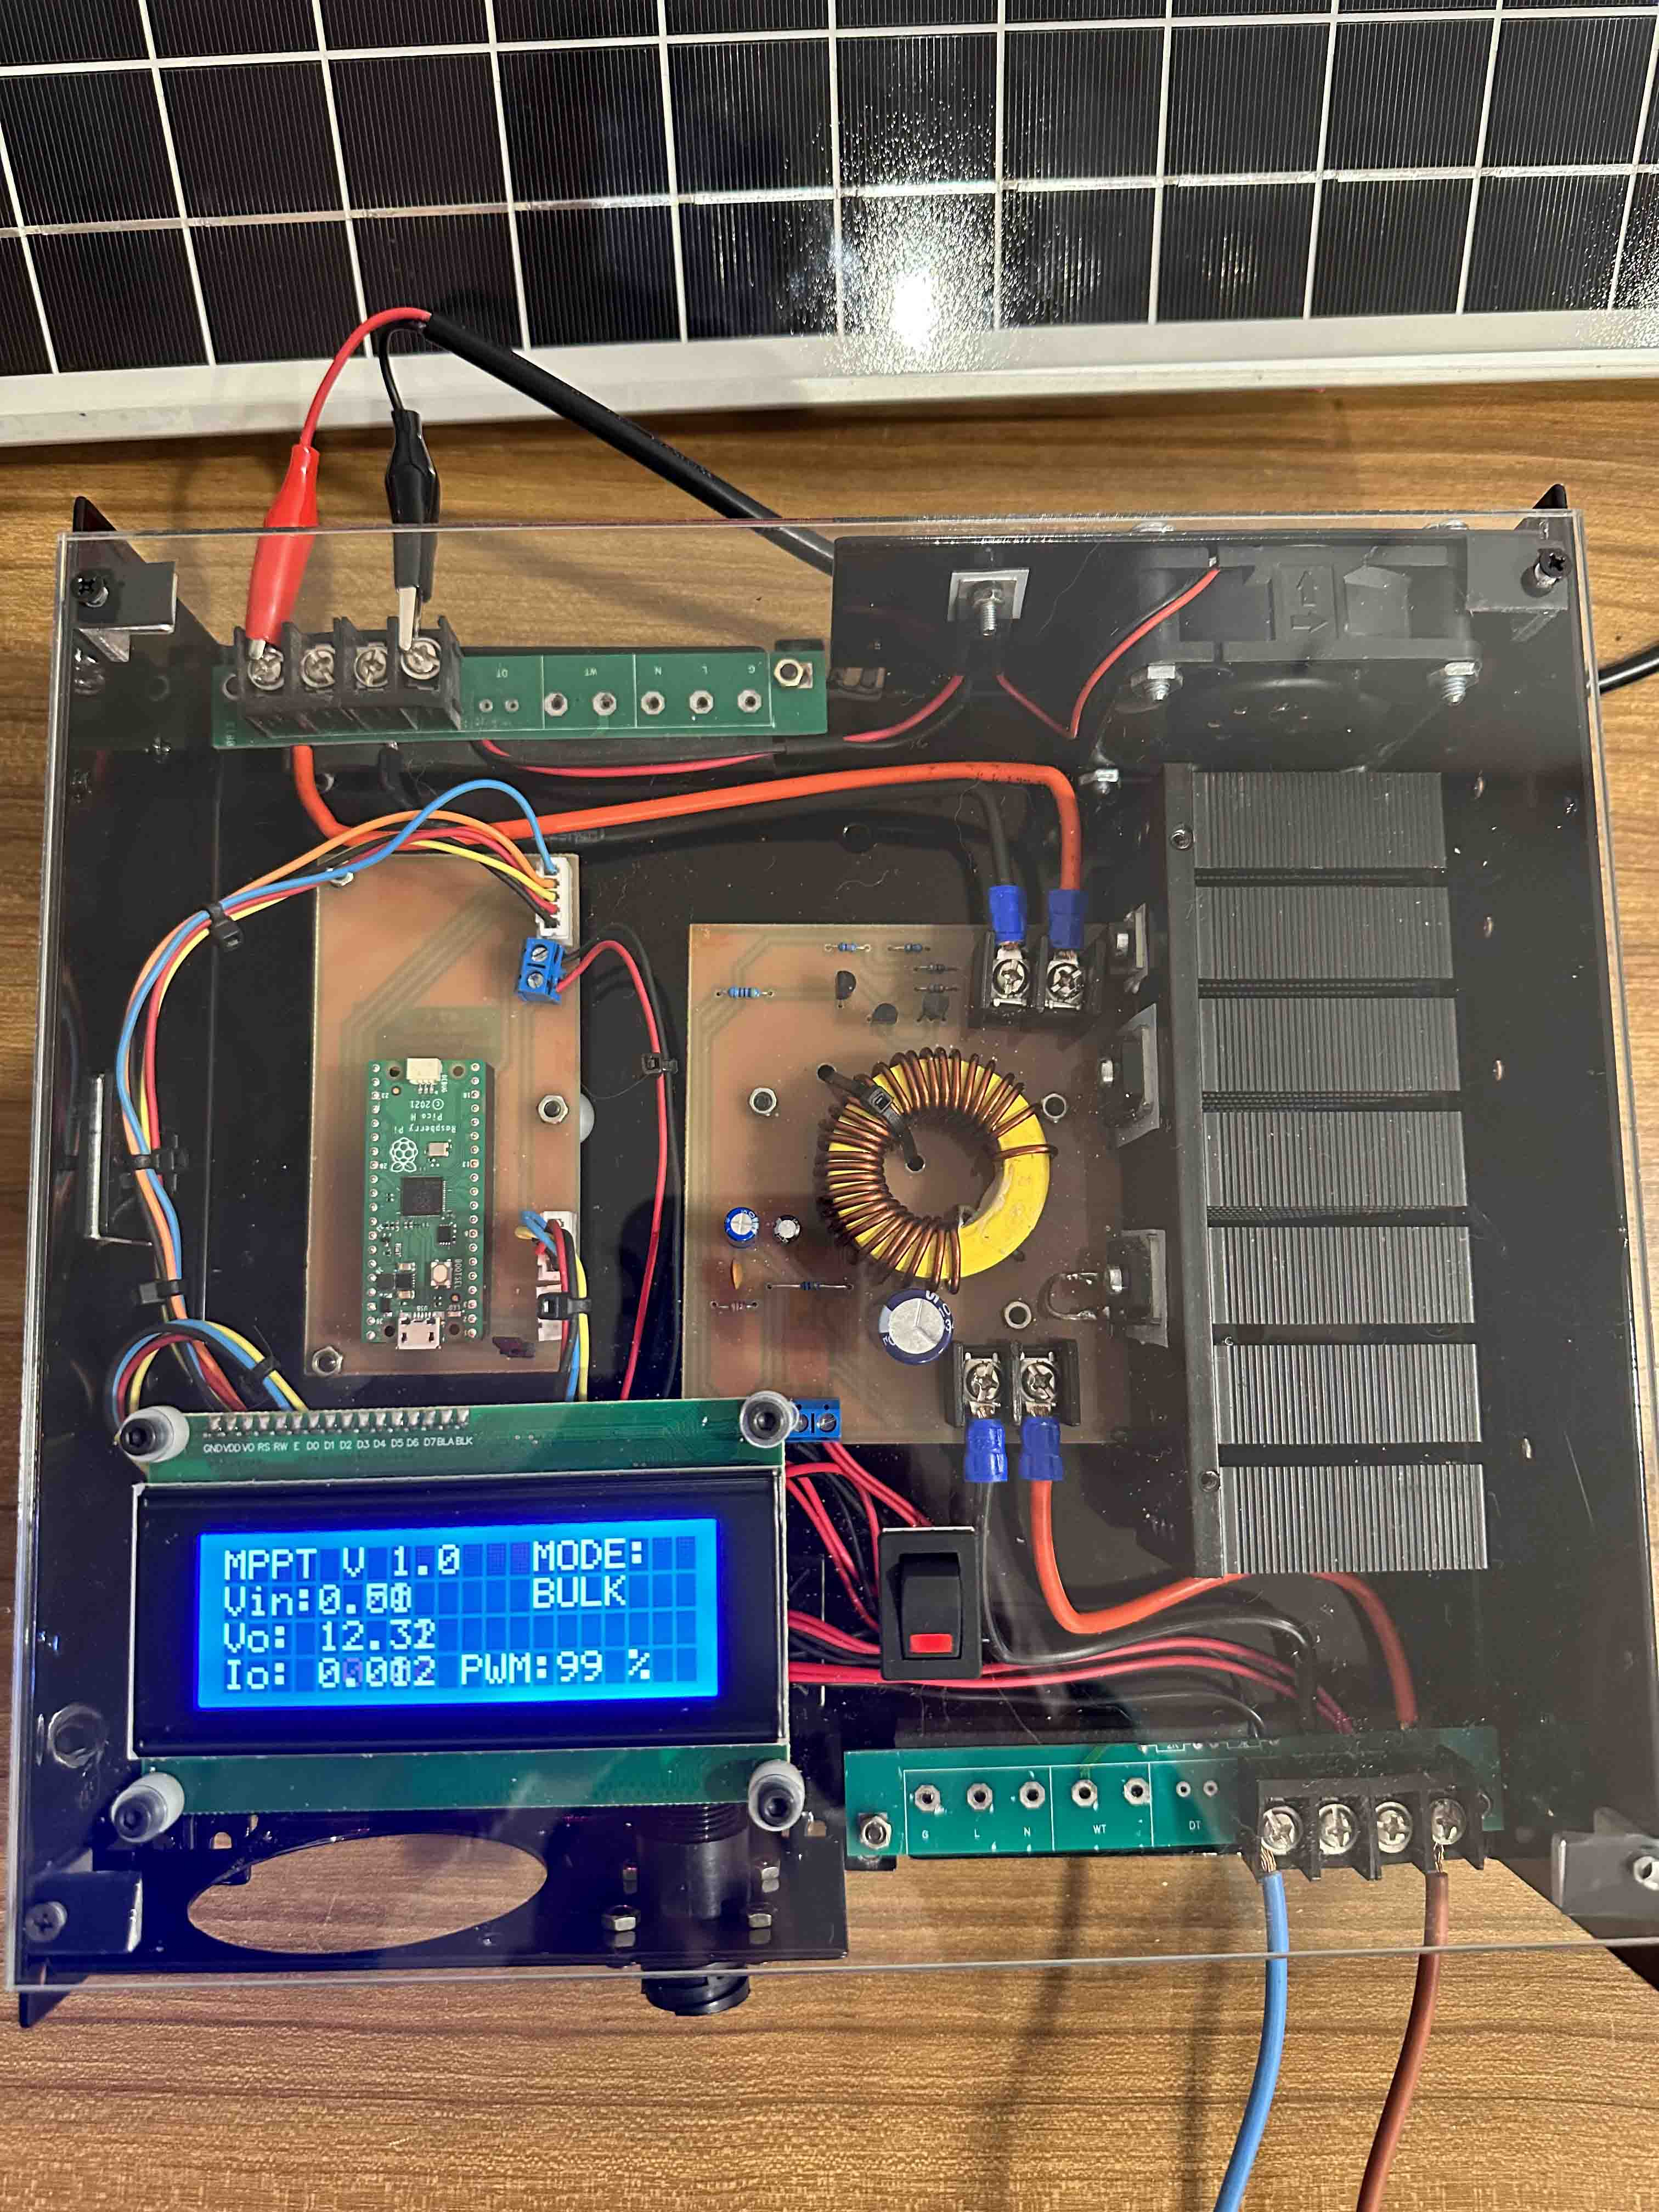
\includegraphics[width=0.9\linewidth]{MPPT/IMG_8032.jpg} 
\caption{Cargador presentado en gabinete.}
\label{fig:MPPT-fin-1}
\end{figure}

\begin{figure}[H]
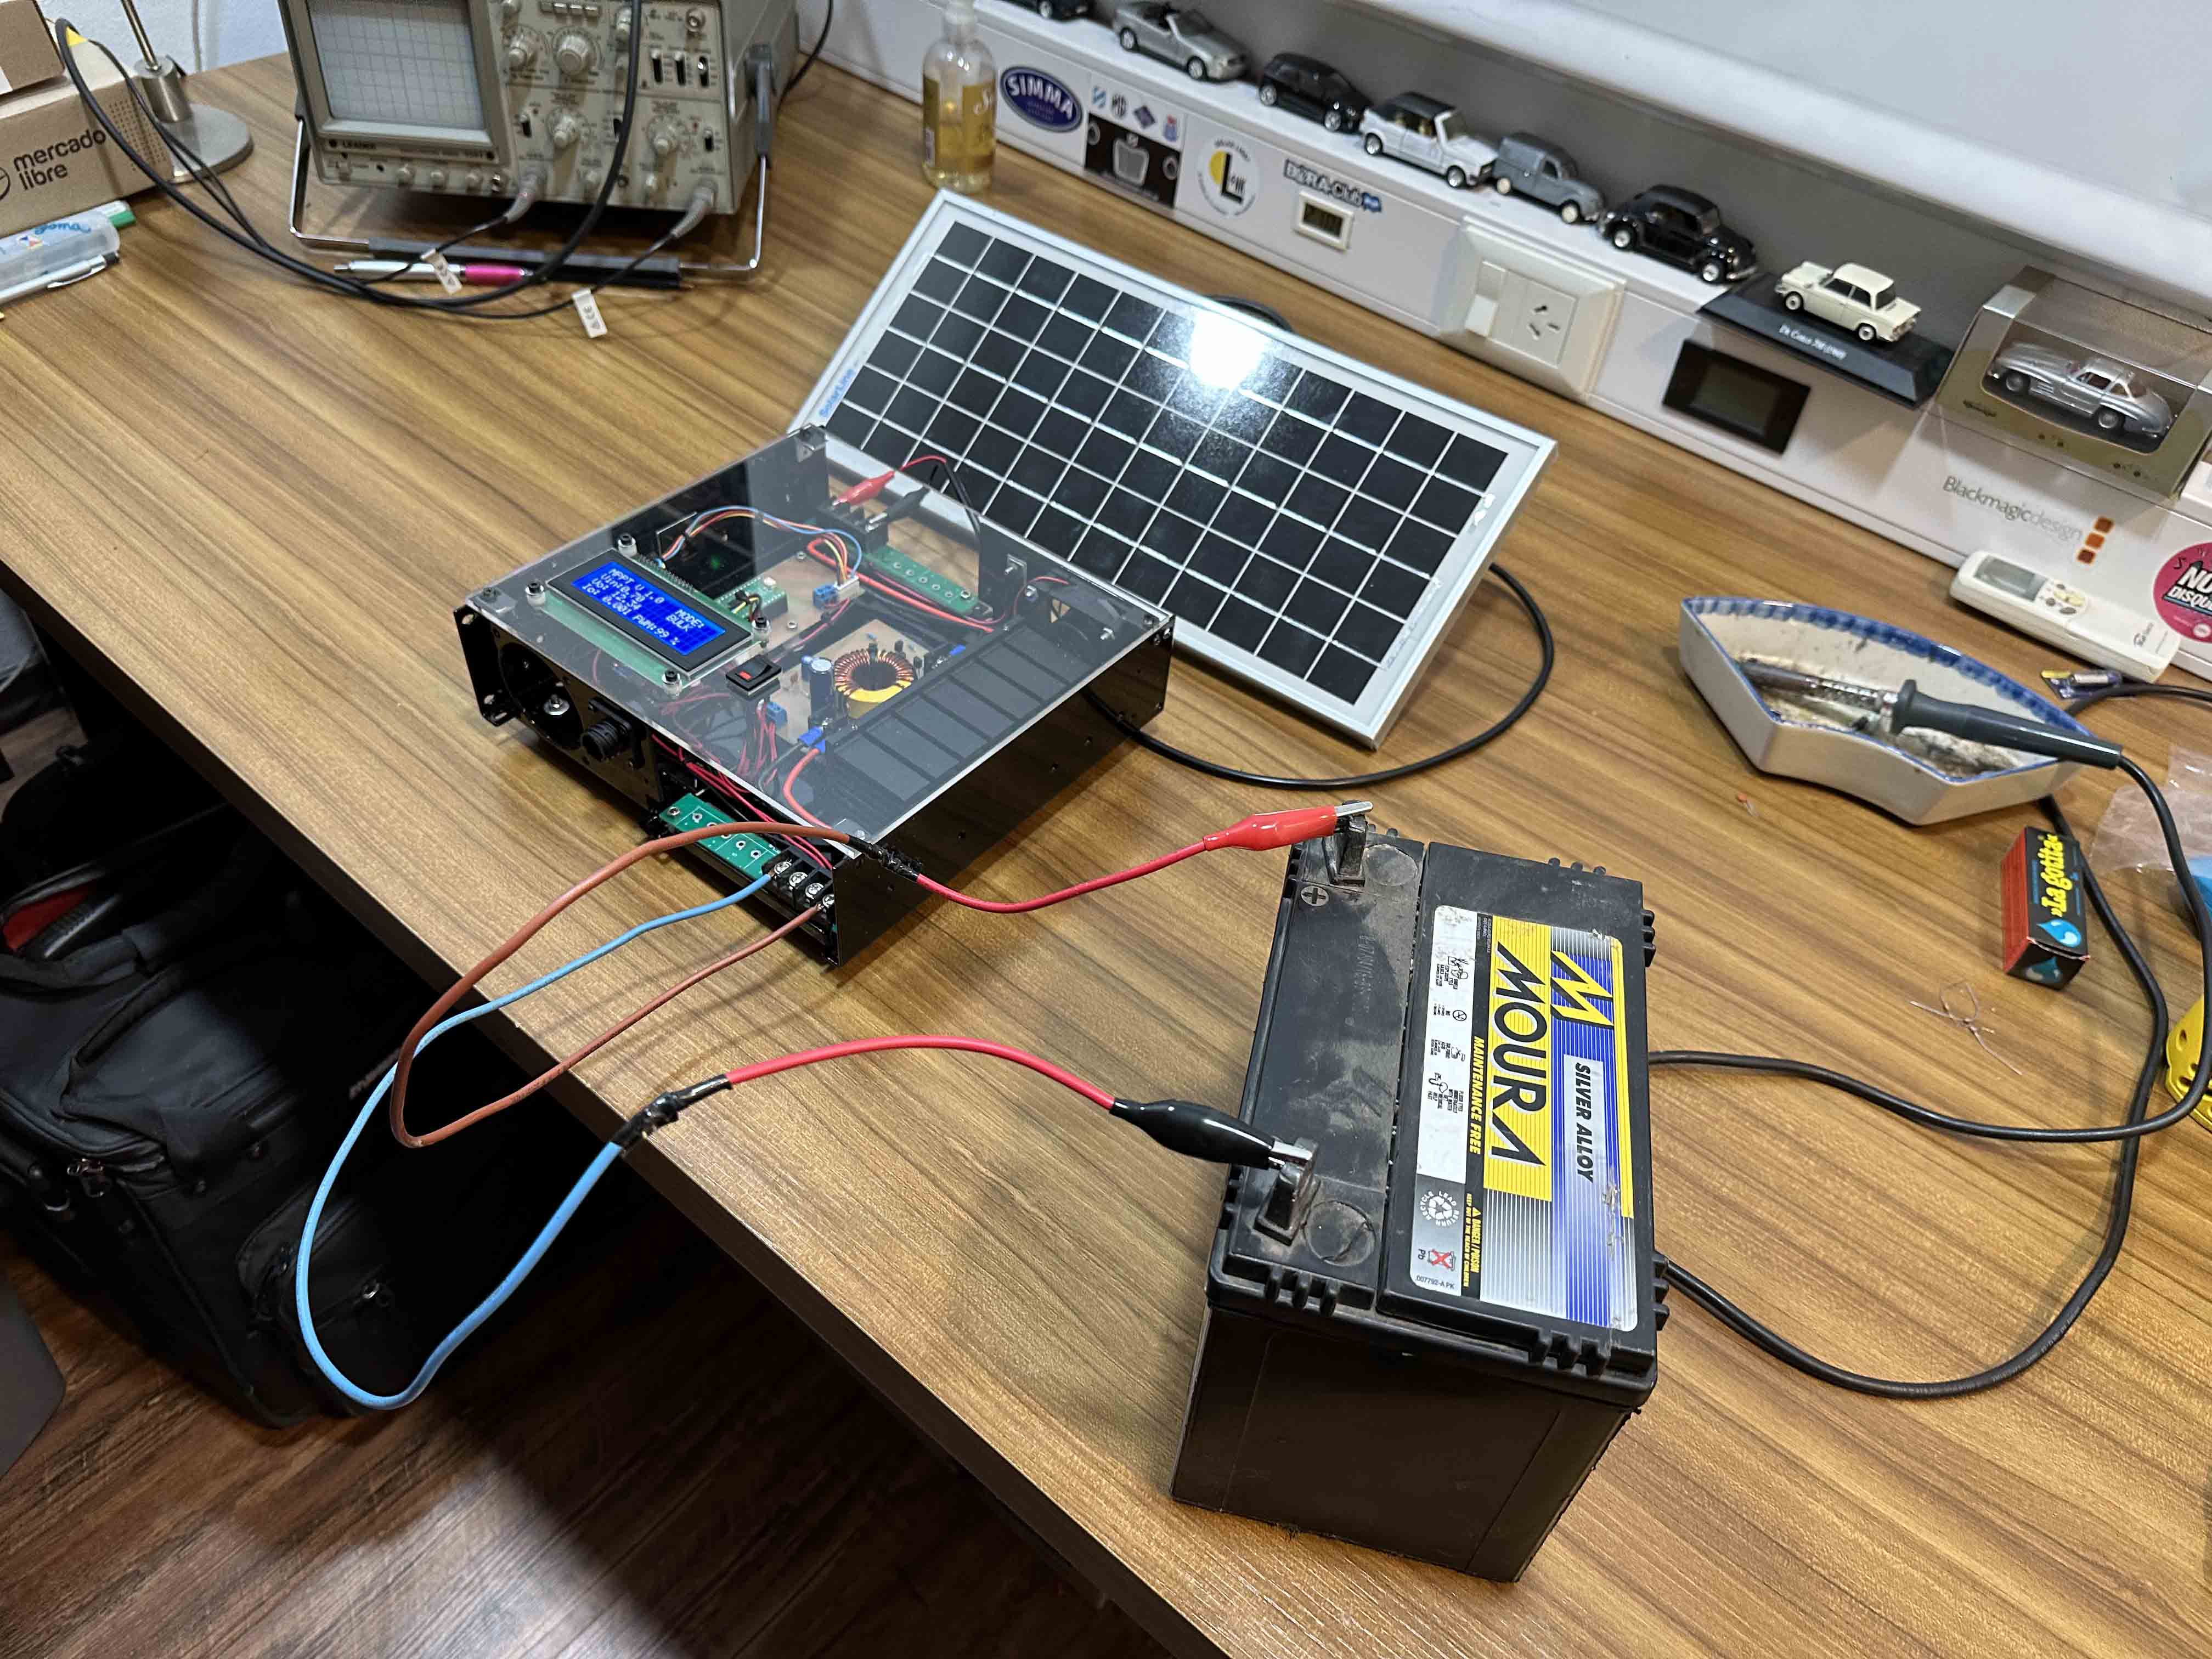
\includegraphics[width=0.9\linewidth]{MPPT/IMG_9390.jpg}
\caption{Cargador en funcionamiento.}
\label{fig:MPPT-fin-2}
\end{figure}

Para su presentación final, se elaboró un gabinete a partir de dos chasis de fuentes switching en desuso, unidas y pintadas, y para la parte superior se utilizó un acrílico para poder ver en su interior. También se le agregó un cooler en la zona del disipador, encargado de extraer calor del gabinete. Este cooler está conectado a traves de otra fuente Step Down a los paneles solares.\\

Como conclusión, se puede decir que es un cargador único en su tipo, aprovechando los últimos avances tecnólogicos para la carga de baterías, logrando una calidad especial en la carga. Este tipo de cargadores que alargan la vida útil de una batería con las 3 etapas de carga, y con una eficiencia por encima del 90\%, no se comercializan actualmente en Argentina.\\

Para finalizar, las mejoras que se pueden realizar en un futuro a este prototipo, se puede agregar un sensor de temperatura para protegerlo frente a un sobrecalentamiento, y un selector de corrientes de carga, siendo que este parámetro es el único que varía realmente entre baterías. De esta forma, quedaría protegido y tendría una opción para cargar diferentes baterías.\\


\subsection{Especificaciones}

Convertidor reductor DC-DC microcontrolado

\begin{itemize}
    \item Voltaje de entrada mínimo: 12Vdc
    \item Voltaje de entrada máximo: 25Vdc
    \item Corriente de entrada máxima: 20A
    \item Voltaje de salida mínimo: 12Vdc
    \item Voltaje de salida máximo: 14,5Vdc
    \item Corriente de salida máxima: 20A
\end{itemize}

\clearpage

\section{Hardware del módulo Solar Link}

\subsection{Esquema general}
El hardware principal de Solar Link se compone de 3 plaquetas principales:

\begin{itemize}
    \item \textbf{Motherboard:} Es donde se encuentra el microcontrolador principal ESP32. Esto implica que es el núcleo del proyecto, y tiene que poder transmitir y recibir información hacia y desde todo el resto de módulos.
    \item \textbf{Medidor de corriente:} Este módulo posee los sensores de corriente no invasivos. A través de estos, podemos medir independientemente la corriente que circula por cada una de las dos líneas que utilizamos.
    \item \textbf{Módulo de conmutación:} Se encarga de switchear entre la línea del proveedor eléctrico y la línea de energía solar.
\end{itemize}

Este hardware se presenta en un tablero eléctrico, el cual reduce al mínimo las interferencias por ruido eléctrico, y permite que el sistema quede protegido frente al uso diario.\\

Este tablero también posee, a modo de prototipo, dos entradas de línea, una se conecta a la red eléctrica convencional, y otra a la línea de energía solar, dos salidas independientes, las cuales son dos zapatillas representando la línea de una casa, y una ficha de comunicación, la cual se conecta al cargador MPPT para recibir información sobre la carga de la batería. Además, posee una antena WIFI para la ESP32.\\

El sistema es alimentado por dos transformadores 220V-9+9V, uno para la motherboard y el medidor de corriente, y otro exclusivo para el módulo de conmutación. Fue necesario el uso de un transformador exclusivo para esta última placa debido al alto consumo que representan los relés.\\

La señal entrante se rectifica con el circuito de la figura \ref{fig:Fuente 12v}, el cual, utilizando el punto medio de los transformadores, rectifica la señal de 9V de alterna, convirtiéndola en una de aproximadamente 12V.\\

\begin{figure}[H]
    \centering
    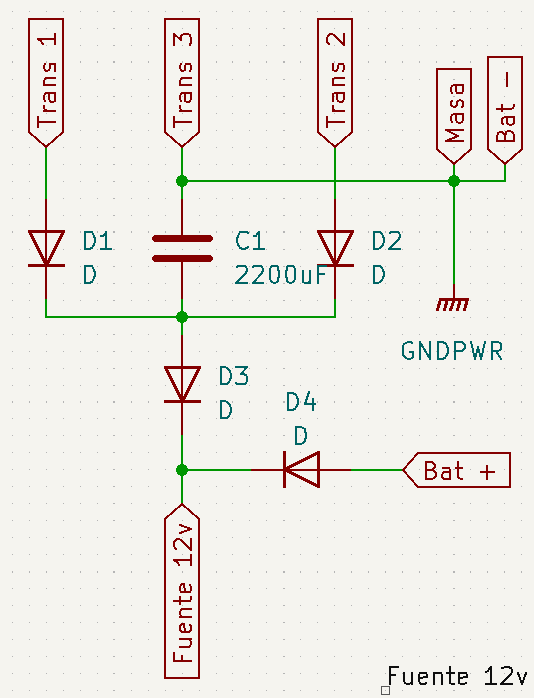
\includegraphics[width=0.7\linewidth]{hardware/Screenshot_10.png}
    \caption{Fuente 12V de Solar Link para los relés.}
    \label{fig:Fuente 12v}
\end{figure}

Por otra parte, a este circuito también entran los 12V de la batería. Gracias a los diodos en el circuito, la señal de salida resultará de la fuente con mayor potencial. De esta manera, frente a un corte de suministro eléctrico, el sistema seguirá funcionando con la energía de la batería.\\

Para mostrar la información medida, utilizamos un LCD de 20x04, colocado en la tapa del tablero. De esta manera, se pueden visualizar estos valores a simple vista sin tener que acceder a la aplicación o necesidad de abrir el tablero mismo.\\

\subsection{Motherboard}

\subsubsection{Sistema embebido}

El núcleo de nuestro proyecto es el microcontrolador ESP32. Es una placa de desarrollo que y trabaja con el microprocesador Tensilica Xtensa LX6 de 32 bits y 2 núcleos. Además, cuenta con periféricos como UART, I2C, ADC, Wi-Fi, Bluetooth, entre otros.\\

\begin{figure}[H]
    \centering
    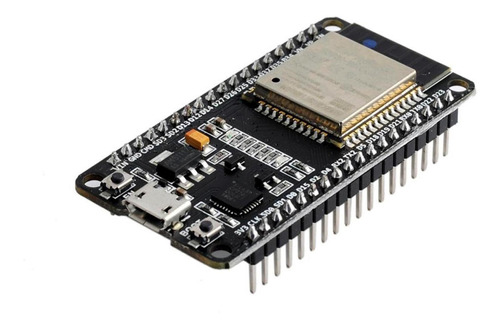
\includegraphics[width=0.75\linewidth]{hardware/ESP32.jpg}
    \caption{Placa de desarrollo ESP32 Devkit V 1.0}
    \label{fig:ESP32}
\end{figure}

Esta placa cuenta con 2 ADC internos de 12 bits de resolución, los cuales pueden trabajar hasta con 15 entradas diferentes. Se realizan únicamente 2 mediciones con ADCs, voltaje de batería y de línea, por lo tanto se asigna cada una a un ADC diferente, optimizando el uso de ambos para lograr mejores mediciones.\\

El periférico de comunicación I2C se utiliza para comunicarse con el ADC externo ADS1115 (figura \ref{fig:ads1115}), y para el LCD de 20x04. Por otra parte, el periférico de comunicación UART es utilizado para recibir información de la Raspberry Pi Pico del cargador MPPT.\\

El módulo Wi-Fi es utilizado para transmitir toda la información recabada hacia la aplicación, la cual se encarga de organizarla para que se pueda visualizar de una manera agradable y entendible.\\

Se aprovechan los dos núcleos del microprocesador para realizar todas las mediciones y comunicaciones en uno, y en el otro enviar la información por medio de Wi-Fi. Esto, en caso de un fallo en este módulo, no se congele el resto de instrucciones, además de poder realizarlas con mayor velocidad por estar distribuidas.\\

\subsubsection{Mediciones realizadas}

En la motherboard de Solar Link, se realizan 3 mediciones independientes: voltaje de línea, voltaje de batería, y cruce por cero.\\

Para medir el voltaje de línea, se utiliza el circuito de la figura \ref{fig:Vlinea}. Este cuenta con un rectificador de media onda y un capacitor conectados a la salida del tranformador, resultando en un voltaje de continua proporcional al voltaje de la línea de la casa. Como el valor de esa señal de continua es muy grande, se utiliza un divisor resistivo que disminuye la tensión en una escala donde el ADC lo puede leer sin problema.\\

\begin{figure}[H]
    \centering
    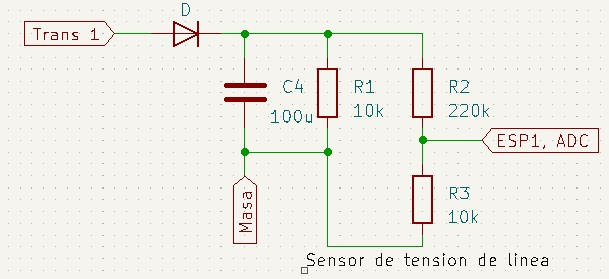
\includegraphics[width=0.9\linewidth]{hardware/Screenshot_14.jpg}
    \caption{Circuito de medición de tensión de línea.}
    \label{fig:Vlinea}
\end{figure}

El voltaje de la batería, al ya ser una señal de continua, simplemente se utiliza un divisor de tensión para medirlo (figura \ref{fig:Vbat}). Si bien este valor tambien lo lee y comparte el cargador, se mide por seguridad, puesto que es algo que se tiene que tener en cuenta para la lógica de conmutación, y si por alguna razón falla o se desconecta el cargador externo, esta lógica fallaría, pudiendo causar daños al hogar y al sistema solar.\\

\begin{figure}[H]
    \centering
    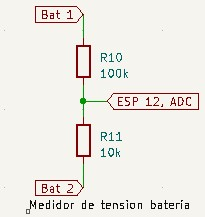
\includegraphics[width=0.5\linewidth]{hardware/Screenshot_16.jpg}
    \caption{Circuito de medición de baterías.}
    \label{fig:Vbat}
\end{figure}

El cruce por cero se mide con un circuito comparador (figura \ref{fig:cruce-cero}). Se toma la señal de alterna del transformador, y se compara con 0 constantemente. Cada vez que dicha señal cruce por cero, la salida de este circuito intercala flancos ascendentes y descendentes.\\

\begin{figure}[H]
    \centering
    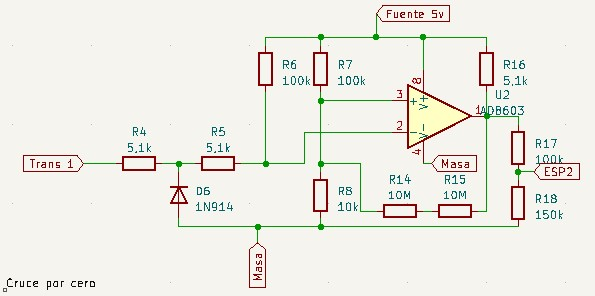
\includegraphics[width=0.9\linewidth]{hardware/Screenshot_15.jpg}
    \caption{Circuito cruce por cero.}
    \label{fig:cruce-cero}
\end{figure}

\begin{figure}[H]
    \centering
    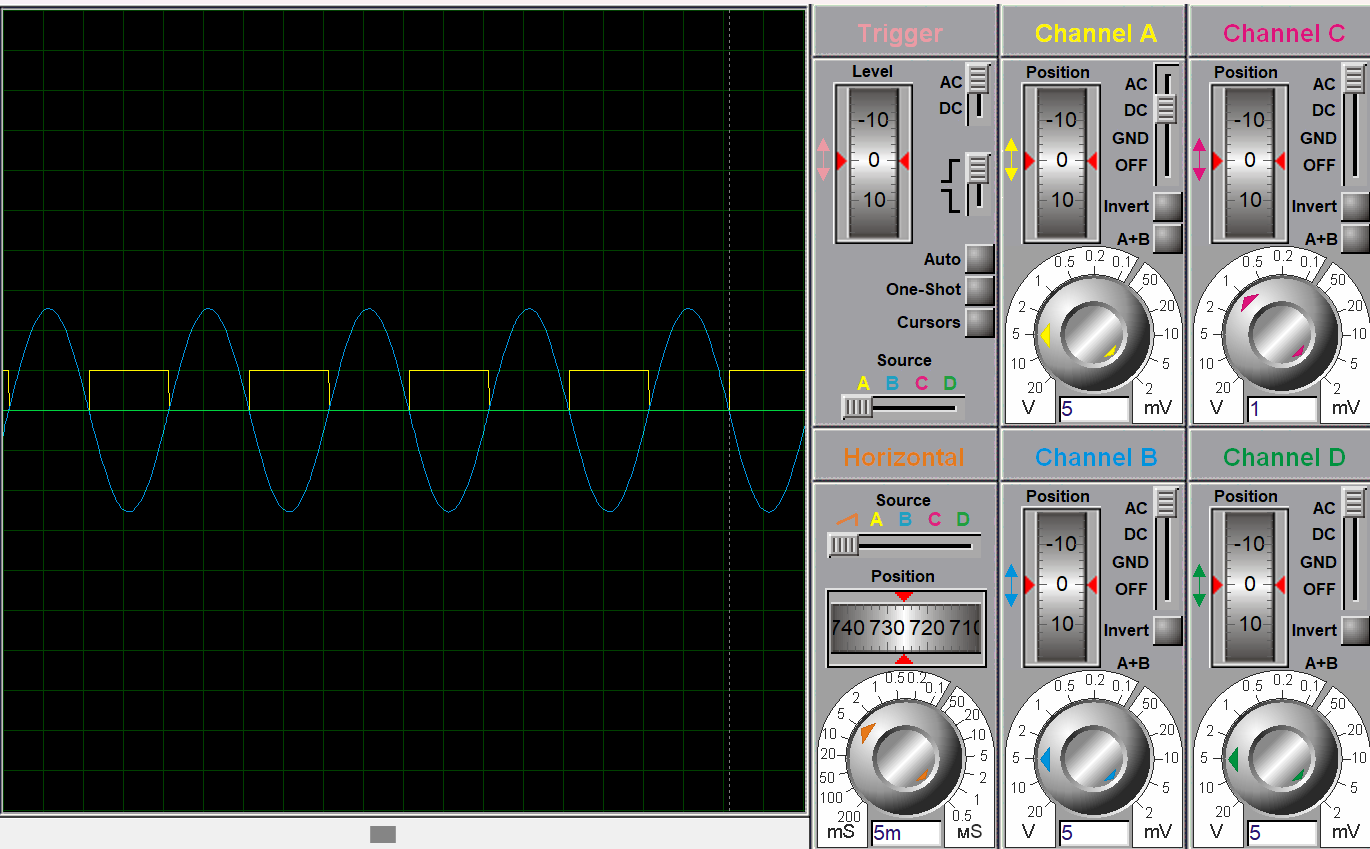
\includegraphics[width=1\linewidth]{hardware/Screenshot_26.png}
    \caption{Salida del circuito cruce por cero.}
    \label{fig:cruce,cero}
\end{figure}

\subsubsection{Alimentación}

La motherboard posee dos entradas de alimentación: batería ($\approx$12V dc) y transformador (9+9V ac).\\

Utilizando el mismo circuito que para alimentar el circuito de conmutación (figura \ref{fig:Fuente 12v}), el sistema puede seguir siendo utilizado frente a cortes en el suministro eléctrico. La motherboard posee un transformador exclusivo para que la lectura de tensión se vea lo menos afectada posible por consumos altos en la salida del mismo (estos provocan caídas en la tensión de salida).\\

Para alimentar el microcontrolador, junto al LCD de 20x04, y al ADC externo ADS1115, se requieren 5Vdc. Para esto, se utilizó un regulador de tensión LM7805, cuya entrada de almentación es la salida de la fuente de 12V, y su salida se conecta a los dispositivos mencionados. Además, la motherboard incluye una salida de 5V en una bornera, por si es necesario su uso en otro periférico.\\

\subsubsection{Resultado final}

\begin{figure}[H]
    \centering
    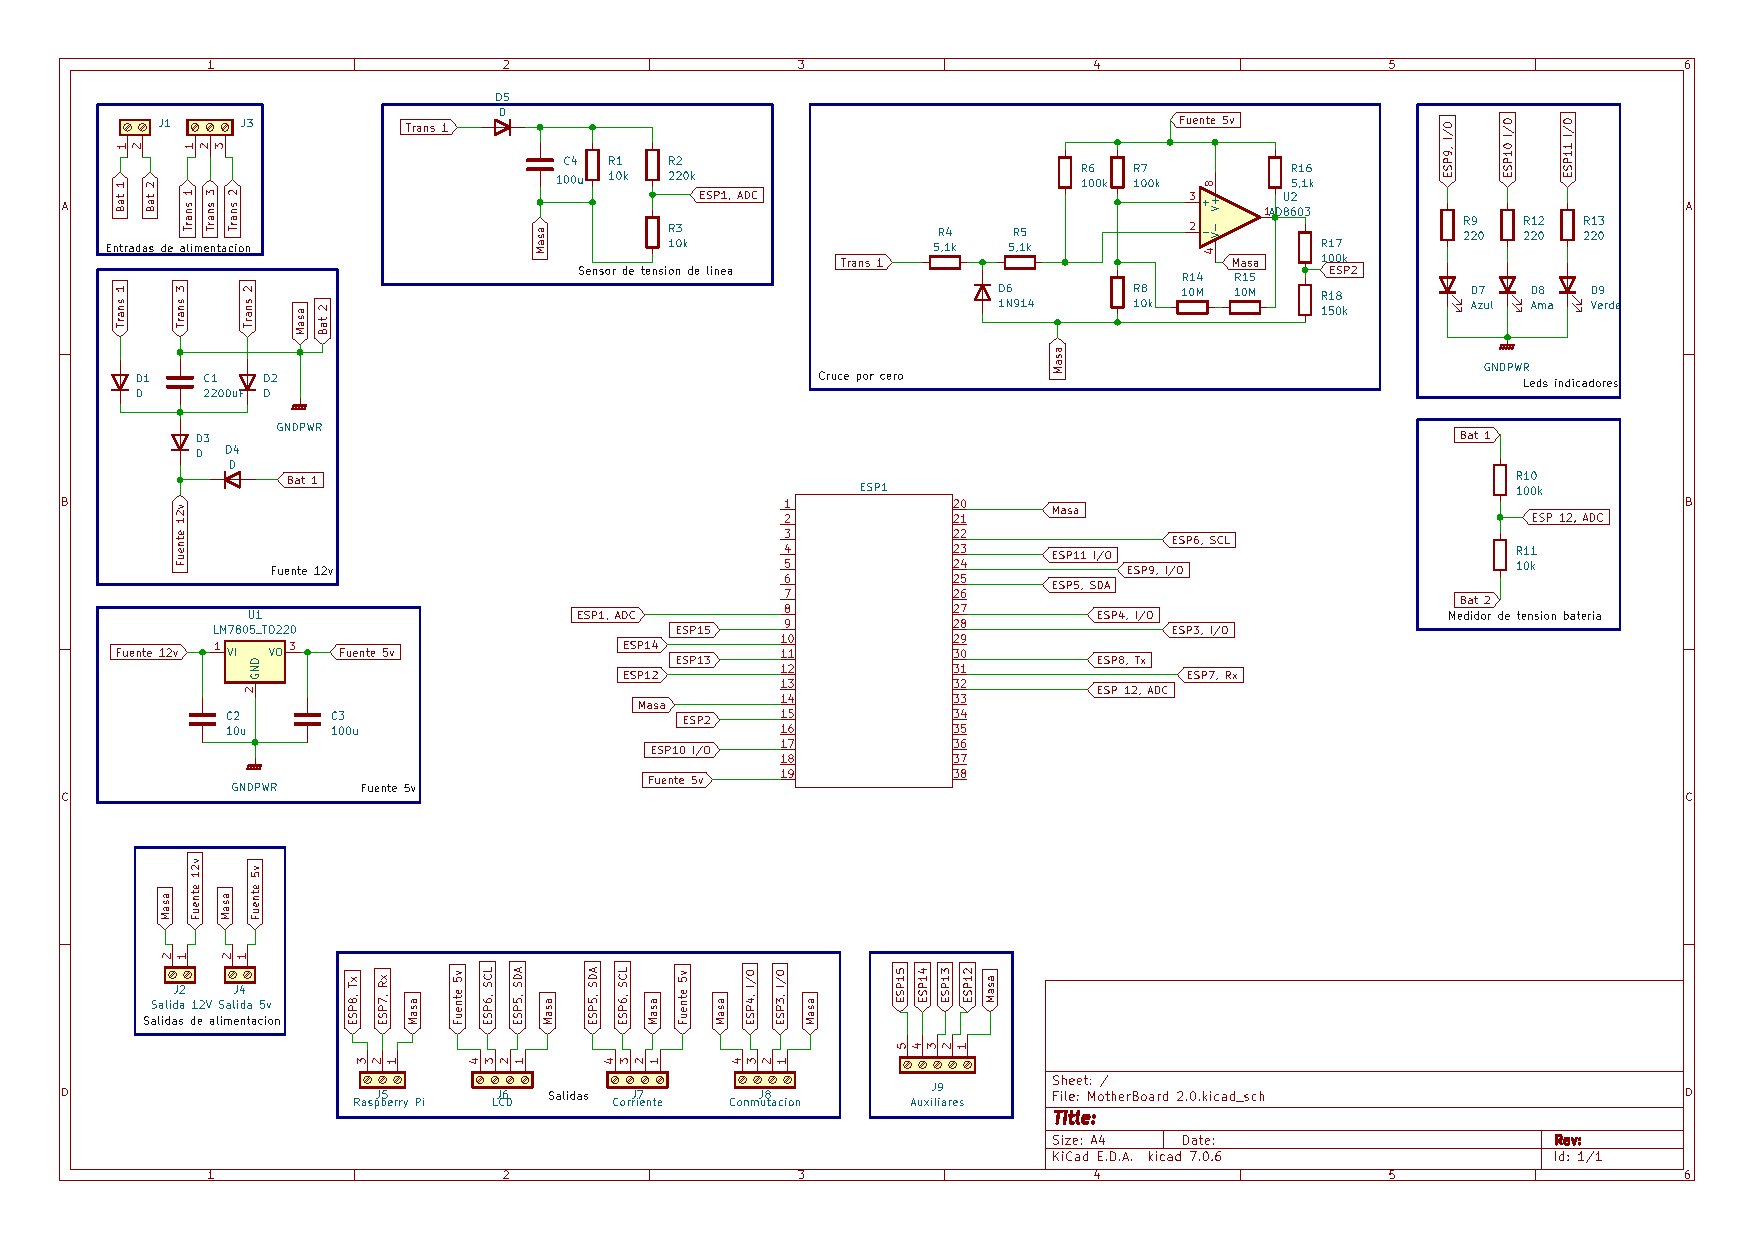
\includegraphics[width=1\linewidth]{hardware/MotherBoard 2.0.pdf}
    \caption{Diseño esquemático final de la motherboard.}
    \label{fig:mother-sch}
\end{figure}

\begin{figure}[H]
    \centering
    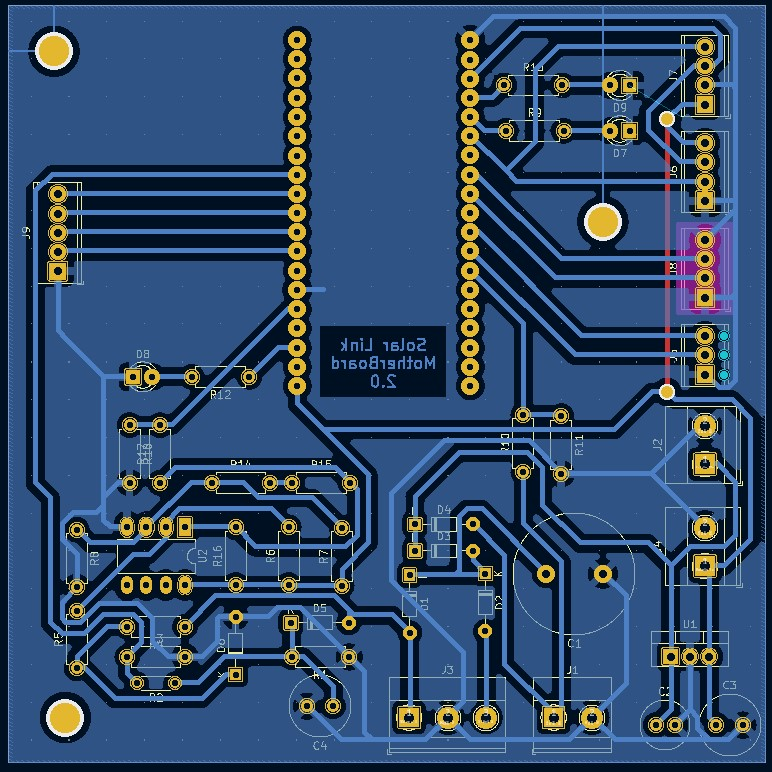
\includegraphics[width=0.7\linewidth]{hardware/Screenshot_17.jpg}
    \caption{Diseño del PCB final de la motherboard.}
    \label{fig:mother-pcb}
\end{figure}

\begin{figure}[H]

\begin{subfigure}{0.5\textwidth}
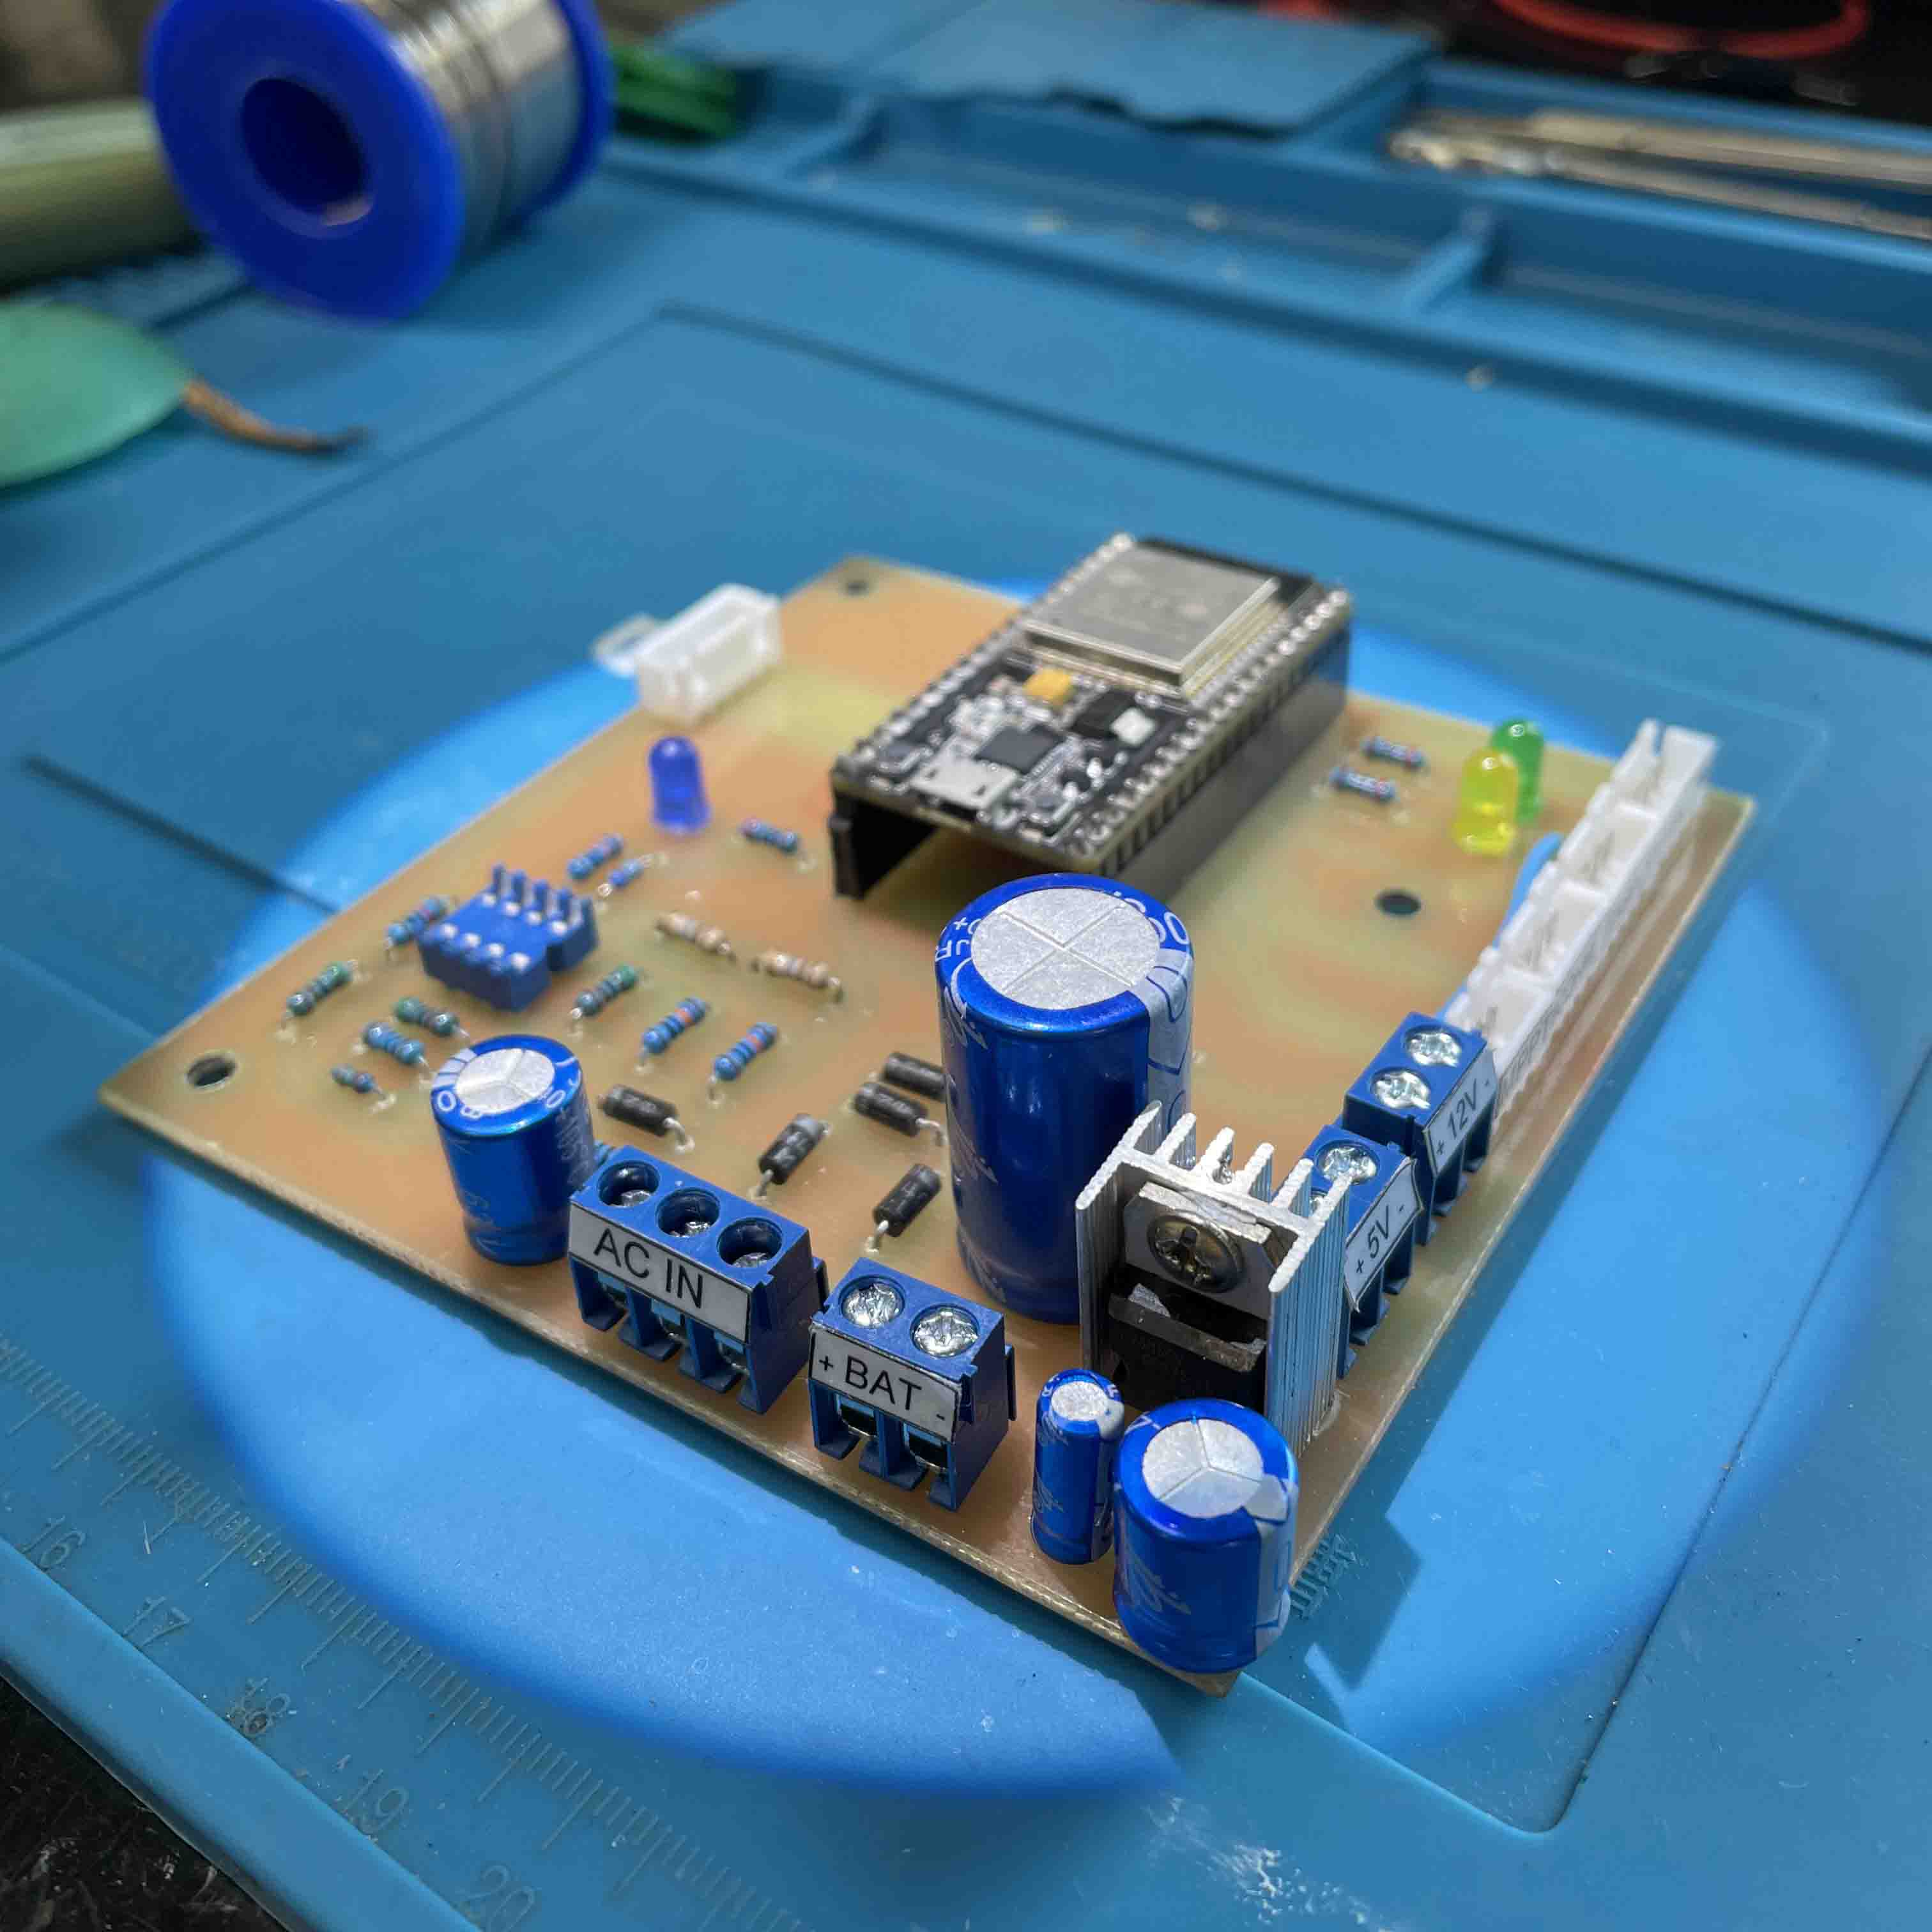
\includegraphics[width=0.9\linewidth]{hardware/IMG_8945.jpg} 
\caption{Plaqueta final motherboard.}
\label{fig:corr-fin}
\end{subfigure}
\begin{subfigure}{0.5\textwidth}
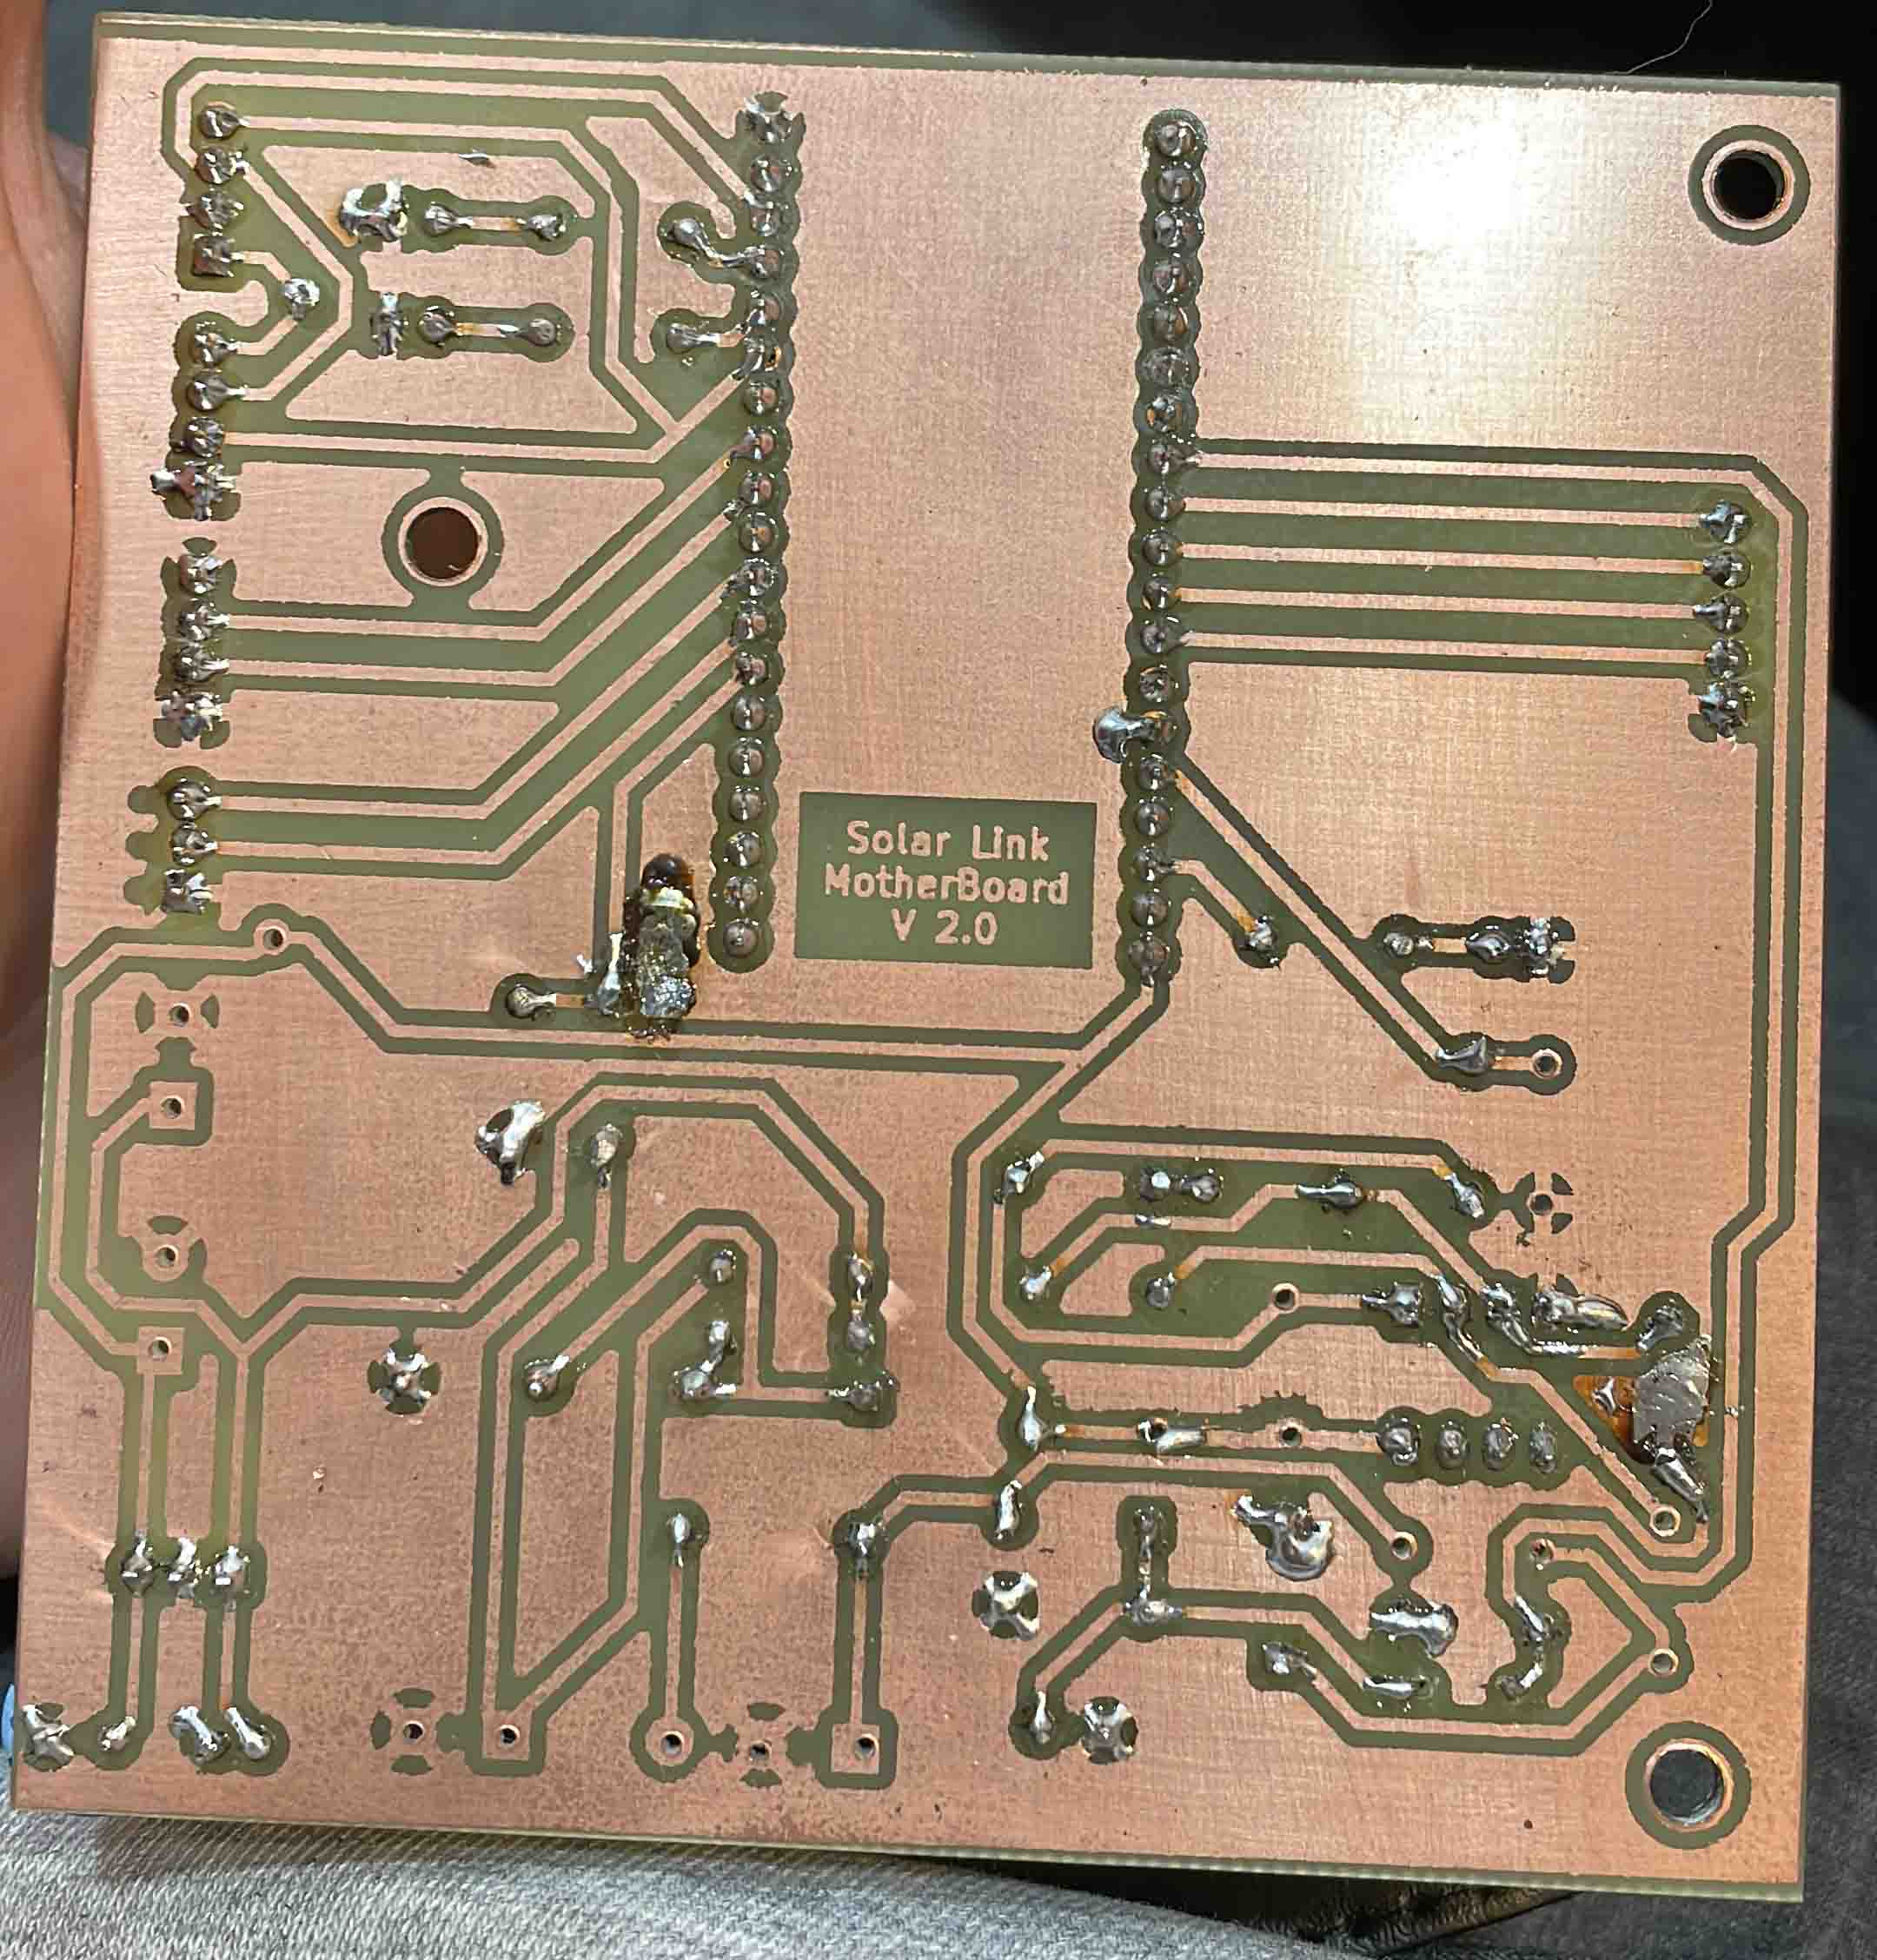
\includegraphics[width=0.9\linewidth]{hardware/F44CD098-7B36-40C0-95DB-D5040B6878EF.JPG}
\caption{Plaqueta motherboard lado inferior.}
\label{fig:corr-pcb}
\end{subfigure}

\caption{Resultados finales de la motherboard.}
\label{fig:corriente-fin}
\end{figure}

\subsection{Medidor de corriente}

\subsubsection{Explicación del circuito}

Para medir la corriente, utilizamos los sensores HW-666, cuya principal ventaja es que son no invasivos. Esto quiere decir que no tenemos que intervenir directamente en la línea eléctrica para realizar las mediciones.\\

\begin{wrapfigure}{l}{0.3\textwidth}
\includegraphics[width=0.9\linewidth]{hardware/hw666.jpg} 
\caption{Sensor de corriente HW-666}
\label{fig:hw666}
\end{wrapfigure}

Estos sensores son unos transformadores de corriente con una relación de vueltas de 1000:1. Cuando se le introduce un cable por su orificio, la corriente que circule en este será inducida en el sensor. Como tiene en paralelo una resistencia de 100$\Omega$, la corriente inducida en el transformador circulará por la resistencia, resultando en un voltaje proporcional.\\

% \begin{wrapfigure}{b}{0.3\textwidth}
% \includegraphics[width=0.9\linewidth]{hardware/ads1115.jpg} 
% \caption{ADC externo ADS1115}
% \label{fig:ads1115}
% \end{wrapfigure}

El voltaje que devuelve el sensor es de una señal alterna, que varía entre semiciclos positivos y negativos. Por lo tanto, para medir esta señal se requiere de un ADC diferencial, que permite la medición tanto de voltajes positivos como negativos.\\

Para esto utilizamos el ADC externo ADS1115, de 16 bits de resolución, que posee 4 entradas de ADC, pudiendo utilizarlas de a pares en modo diferencial, es decir, 2 entradas de ADC diferencial.\\

\begin{figure}[H]
    \centering
    \includegraphics[width=0.5\linewidth]{hardware/ads1115.jpg}
    \caption{ADC externo ADS1115}
    \label{fig:ads1115}
\end{figure}

Este ADC procesa la señal y se la transmite al microcontrolador a través del protocolo de comunicación I2C.\\

\subsubsection{Resultado final}

\begin{figure}[H]
    \centering
    \includegraphics[width=0.9\linewidth]{hardware/Screenshot_11.png}
    \caption{Diseño de esquemático.}
    \label{fig:sch-corr}
\end{figure}

\begin{figure}[H]
    \centering
    \includegraphics[width=0.9\linewidth]{hardware/Screenshot_12.png}
    \caption{Diseño de PCB.}
    \label{fig:pcb-corr}
\end{figure}

\begin{figure}[H]

\begin{subfigure}{0.5\textwidth}
\includegraphics[width=0.9\linewidth]{hardware/IMG_8066.jpg} 
\caption{Plaqueta final medidor de \\corriente.}
\label{fig:corr-fin}
\end{subfigure}
\begin{subfigure}{0.5\textwidth}
\includegraphics[width=0.9\linewidth]{hardware/IMG_8587.jpg}
\caption{Plaqueta final medidor de corriente \\lado inferior.}
\label{fig:corr-pcb}
\end{subfigure}

\caption{Resultados finales del medidor de corriente.}
\label{fig:corriente-fin}
\end{figure}

Con una correcta calibración, resulta ser un módulo de medición muy preciso tanto en pequeñas como grandes escalas. Como lo estipula el fabricante, la máxima corriente que puede medir sin empezar a dar valores erróneos ronda en los 10A.

\clearpage

\subsection{Módulo de conmutación}

\subsubsection{Explicación del circuito}

Para conmutar entre líneas utilizamos los relés de potencia inversores HJQ-15F-S-Z, que con un simple pulso nos permite cambiar entre sus terminales normal cerrado y normal abierto.\\

\begin{figure}[H]
    \centering
    \includegraphics[width=0.4\linewidth]{hardware/Rele.jpg}
    \caption{Relé HJQ-15F-S-Z}
    \label{fig:rele}
\end{figure}

Para conmutar estos relés, fue necesario utilizar el circuito de la figura \ref{fig:opto-mosfet-rele}. Este circuito cuenta con un MOSFET IRFZ44N encargado de conmutar la alimentación de la bobina del relé, y un optoacoplador para alimentar el gate del MOSFET con la señal entrante del ESP32. \\

\begin{figure}[H]
    \centering
    \includegraphics[width=0.9\linewidth]{hardware/Screenshot_19.jpg}
    \caption{Circuito de conmutación.}
    \label{fig:opto-mosfet-rele}
\end{figure}

Utilizamos el optoacoplador para aislar el microcontrolador del circuito de potencia. En caso de una falla eléctrica, el ESP32 no se vería afectado y seguiría funcionando sin problema.\\

\subsubsection{Resultado final}

\begin{figure}[H]
    \centering
    \includegraphics[width=1\linewidth]{hardware/Screenshot_18.jpg}
    \caption{Diseño final PCB de conmutación.}
    \label{fig:conmutacion-pcb}
\end{figure}

\begin{figure}[H]

\begin{subfigure}{0.5\textwidth}
\includegraphics[width=0.9\linewidth]{hardware/IMG_8220.jpg} 
\caption{PCB final de conmutación.}
\label{fig:conm-fin}
\end{subfigure}
\begin{subfigure}{0.5\textwidth}
\includegraphics[width=0.9\linewidth]{hardware/IMG_8221.jpg}
\caption{PCB final de conmutación por debajo.}
\label{fig:conm-inf}
\end{subfigure}

\caption{Resultado final del módulo de conmutación.}
\label{fig:image2}
\end{figure}

Este módulo, si bien funciona como debe a la perfección, para nuestro uso presenta un desperfecto: cuando el relé realiza la comutación, hay un punto muerto donde no hay ningún tipo alimentación. Si bien esto se compensa en parte por el cruce por cero, sigue siendo un desperfecto con el cual debemos lidiar.

\subsection{Diseño 3D}
Para presentar el prototipo final en el tablero, fue necesario diseñar una carcasa 3D para cada plaqueta, de tal manera que puedan ser colocadas en un riel DIN y queden protegidas. Cada carcasa fue diseñada especialmente para cada plaqueta, con orificios en los laterales para poder realizar las conexiones, y dejando la parte superior abierta para colocar un acrílico que permita verlas en funcionamiento.\\

\begin{figure}[H]
    \centering
    \includegraphics[width=0.75\linewidth]{hardware/Screenshot_22.png}
    \caption{Carcasa 3D para la motherboard.}
    \label{fig:mother-3d}
\end{figure}

\begin{figure}[H]
    \centering
    \includegraphics[width=0.75\linewidth]{hardware/Screenshot_21.png}
    \caption{Carcasa 3D para el módulo de medición de corriente.}
    \label{corriente-3d}
\end{figure}

\begin{figure}[H]
    \centering
    \includegraphics[width=0.75\linewidth]{hardware/Screenshot_20.png}
    \caption{Carcasa 3D para el módulo de conmutación.}
    \label{fig:conmutacion-3d}
\end{figure}

\subsection{Disposición final}

Para armar el tablero, se diseñó una disposición donde la electrónica mas delicada que utilizamos (sobre todo el microcontrolador) quede lo más alejado y aislado posible de la parte de potencia del tablero (principalmente el módulo de conmutación).\\ 

Para lograr la máxima prolijidad posible se utilizaron borneras Zoloda y pasacables, de esta manera se logra que haya muy pocos cables a la vista, y si los hay, es por tramos cortos.\\

\begin{figure}[H]
    \centering
    \includegraphics[width=1\linewidth]{hardware/IMG_9354.jpg}
    \caption{Tablero Solar Link.}
    \label{fig:enter-label}
\end{figure}

\begin{figure}[H]
    \centering
    \includegraphics[width=1\linewidth]{hardware/IMG_9352.jpg}
    \caption{Tablero Solar Link con los cablecanales destapados.}
    \label{fig:enter-label}
\end{figure}



\clearpage

\section{Programación del microcontrolador ESP32}

\subsection{Introducción}

El ESP32 es el microcontrolador principal del proyecto, y se encuentra instalado en la motherboard. Las señales utilizadas por el hardware del proyecto son medidas por los sensores de la motherboard y procesadas por el microcontrolador. A su vez, el microcontrolador se encarga de controlar y operar el hardware. La ESP32, además de ser el núcleo “lógico” del sistema, también es el nexo entre los componentes analógicos (principalmente sensores) y la página web, que recibirá, continuará procesando, y mostrará los datos enviados por el microcontrolador, únicos para cada usuario.\\

Este ESP32 es programada en micropython, que es una implementación del lenguaje Python especializada en microcontroladores. Decidimos utilizar Python al ser un lenguaje de alto nivel, con gran amplitud de librerías estándar que facilitan su implementación, convirtiéndolo en un lenguaje sencillo de programar. Aunque, a comparación de c, los programas hechos en python son más lentos, la velocidad de ejecución no representará un obstáculo al funcionamiento correcto del sistema, ya que los procesos que requieren de una rápida ejecución (en este caso, la lógica del cargador MPPT) serán ejecutados sobre las Raspberry Pi Pico, los microcontroladores secundarios del proyecto.\\

El hardware de la motherboard mide los siguientes datos:

\begin{itemize}
    \item Voltaje de la red del proveedor.
    \item Voltaje de batería.
    \item Cruce por cero.
\end{itemize}
Además, recibirá la medición de corriente de cada línea de los sensores de corriente externos.\\

A partir de estos datos, el microcontrolador procesa y calcula la siguiente información:
\begin{itemize}
    \item Promedio de tensión de la red del proveedor.
    \item Picos de corriente de las líneas.
    \item Consumo de cada línea.
\end{itemize}

Con esta información, el microcontrolador hace dos cosas: por un lado, envía la información al servidor de la página web a través de un método POST; el servidor calcula nuevos datos mediante la información recibida, y almacena todo en la base de datos del servidor. Por otro lado, controla el conmutador en base a parámetros definidos: comparando los consumos de la línea con un valor de umbral consumo. Si el consumo medido es inferior al valor de umbral, el microcontrolador acciona el conmutador para que conmute la fuente de la línea a la fuente de energía solar. Si el consumo medido fuese superior al valor de umbral, se conmutará la línea a la red del proveedor eléctrico.\\

Por último, el ESP32 enviará un pulso a la Pi Pico, y ésta le devolverá la información del promedio de consumo en una hora y voltaje de la batería. La comunicación entre ambos microcontroladores se realiza utilizando el protocolo UART; la ESP32 es el microcontrolador master mientras que la Raspberry Pi Pico es el microcontrolador slave.\\ 

La información recibida de parte de la Raspberry Pi Pico también será enviada al servidor web para mostrar al usuario, mientras que la información del voltaje de la batería inhibirá al conmutador de las líneas eléctricas del sistema en caso de ser demasiado baja.\\


\subsection{Librería SolarLink}

La librería “solarlink.py” contiene todas las funciones necesarias para medir la señal de los sensores y manejar los datos del sistema. El programa principal utiliza esta librería para ejecutar tareas específicas. Todo el código base se encuentra en la librería principal del programa para evitar redundancias y para mantener limpio el código del programa principal. Actualmente, la librería consiste de la clase SolarLink.

\subsubsection{Clase SolarLink}

La clase SolarLink contiene las funciones 
\mint{python}|def __init__(self)| 
\mint{python}|def callback_fin_mediciones(self, t)|
\mint{python}|def corriente_dif_read(self, pin a, pin b)|
\mint{python}|def voltaje_read(self)|
\mint{python}|def medicion_default_segundo()|

La función \textbf{init} es el constructor de la librería, que se encarga de configurar e inicializar los ADC interno y externo, el protocolo I2C que habilita la comunicación con el ADC externo; y definir el valor de la pendiente de la corriente en función de la tensión, la referencia del sensor de voltaje, los atributos del Timer, el Callback del timer, y la medición final. Se puede ver su implementación en Listing \ref{main-1} y Listing \ref{main-2}\\

El método \textbf{callback\_fin\_mediciones} tiene como única función setear el atributo \textbf{self.fin\_mediciones} cada vez que se ejecuta el callback del timer, que actúa como flag (Listing \ref{callback-mediciones}).\\

El método \textbf{corriente\_dif\_read} se encarga de obtener la diferencia de voltaje entre los dos pines del ADC externo, al cual le corresponderá cada sensor respectivamente. La diferencia de voltaje es multiplicada por el valor de la pendiente de la corriente en función de la tensión, y dividido por la raíz de dos, obteniendo así el valor de corriente eficaz que luego es devuelto por el método (Listing \ref{clase corriente}).\\

El método \textbf{voltaje\_read} se encarga de medir en microvolts la señal otorgada por el sensor de voltaje, que corresponderá a un valor de tensión eficaz. Luego, este valor se traspasa a volts y se lo multiplica por el valor de referencia del sensor de tensión, así obteniendo el valor equivalente de la tensión de línea. Este dato será la variable devuelta por el método (Listing \ref{clase voltaje}).\\

El método \textbf{medicion\_default\_segundo} realiza múltiples mediciones en un periodo de 1 segundo. El valor devuelto por este método es el dato principal que utilizará el programa main a la hora de realizar tareas específicas (Listing \ref{medicion default segundo}).\\

El bucle principal de la clase se ejecuta de manera constante, y empieza sumando múltiples mediciones de voltaje llamando a \textbf{voltaje\_read}, para promediar el valor posteriormente (Listing \ref{bucle main}).\\

Luego se procede a obtener las mediciones de los dos sensores de corriente, llamando a la función \textbf{corriente\_dif\_read}. Dos bucles if evalúan si la corriente medida es mayor al último pico de corriente registrado, y si no lo es, guarda el valor medido en la variable de pico de corriente, almacenando así los picos máximos de corriente históricos.\\

Un bucle if evalúa la condición del callback del timer. Al pasar un segundo, el callback se setea y se ejecuta el código dentro del bucle. Primero, se saca el promedio de la suma de mediciones de voltaje obtenidas al comienzo del bucle principal de la clase, y se asigna los picos de las dos líneas utilizadas a las variables de valor de corriente respectivos. Se obtiene el consumo de cada línea multiplicando el voltaje promedio por el valor de corriente de cada línea.\\

El \textbf{atributo self.medicion} almacena el valor de voltaje promedio, las corrientes de cada línea, y los consumos de cada línea.\\

Se reinician las variables de picos de corriente, la suma de voltajes, el índice de la suma, y el callback del timer. Finalmente, se rompe el bucle y se retorna el atributo \textbf{self.medicion}.


\subsection{Programa principal}

El programa principal main.py realiza tareas específicas, como el muestreo de datos básicos al display LCD que se encuentra conectado al microcontrolador, el control del conmutador de líneas, y el posteo de los datos al servidor web de SolarLink, que se realiza utilizando las librerías microdot y requests. El programa utiliza la librería SolarLink para obtener los valores de mediciones, llamando a la clase dentro del código principal. Fuera del bucle principal, también se define los pines a los que irán conectados el conmutador, que luego será activado dentro del bucle.

\subsubsection{Bucle principal}

El bucle principal trabaja con los valores devueltos por el método \textbf{medicion\_default\_segundo} de la clase SolarLink. Un display LCD se encarga de mostrar todos los datos devueltos por el método.\\

El diccionario con los valores es convertido a las variables \textit{voltaje}, \textit{corriente\_l1}, \textit{corriente\_l2}, \textit{consumo\_l1}, y \textit{consumo\_l2}. Luego, se colocan en off los pines p\_l1 y p\_l2, que corresponden a los del conmutador. Finalmente, se establece una variable en 100. Esta variable será el threshold de consumo que determinará si se activa el conmutador o no.\\

Un condicional revisa si la suma de la suma de los consumos de ambas líneas es menor al trigger. De ser el caso, conmutará ambas líneas a la red solar. Caso contrario, revisará si el consumo de la primer línea o si el de la segunda es inferior al trigger, y entonces conmutará la línea correspondiente a la red solar. Si ambos consumos son mayores al valor del trigger, entonces conmutará ambas líneas a la red del proveedor.

\subsubsection{Microdot y posteo de datos}

Microdot se encargará de ayudar a decidir a qué usuario le corresponde el módulo Solar Link. Esta pestaña será de visualización sencilla, para no sobrecargar al microcontrolador.

\begin{figure}[H]
    \centering
    \includegraphics[width=1\linewidth]{WhatsApp Image 2023-10-16 at 21.25.50.jpeg}
    \caption{Página de configuración del micro.}
    \label{fig:enter-label}
\end{figure}



\clearpage

\section{Desarrollo de página web}

\subsection{Introducción}

Se requería una página web que pudiera recibir y gestionar los datos de cada módulo Solar Link, como también mostrar esos datos a nombre de un usuario. \\

Luego de una investigación en la que se evaluaron opciones como node.js (un framework o marco de trabajo en javascript) y django (un framework basado en python), se decidió usar django para el backend del proyecto. Esto debido a su amplia variedad de herramientas ya preparadas; la posibilidad de manejar bases de datos sin lenguaje SQL (escribiendo código en python que luego el framework traducía a SQL); el amplio nivel de soporte en internet: secciones de código ya armadas de ejemplo y la posibilidad de usar cualquier librería o módulo de python de terceros sin tener que hacer ningún cambio extra; los conocimientos previos de python por parte de los integrantes; y la posibilidad de utilizar bloques lógicos de python en código HTML, permitiendo cambiar las vistas de la página web con condiciones y bucles.\\

Luego de definir eso, se creó el repositorio de GitHub para poder trabajar en equipo en la página web y tener un registro de los avances. También se hizo una investigación profunda de django para saber cómo encarar el desarrollo y una futura aplicación de Android.\\


\subsection{Django}
Django es un framework (marco de trabajo) basado en python. Está centrado en tener herramientas que faciliten programar y unifiquen todo en el mismo lenguaje de programación. Se basa en el concepto MVC, o vista-modelo-controlador.\\

\begin{figure}[H]
    \centering
    \includegraphics[width=1\linewidth]{web/MVC3.png}
    \caption{Lógica manejada en la página web.}
    \label{fig:arch-mvc}
\end{figure}

Aunque en Django a la vista se le llama template y al controlador se le llama vista.
Aquí, las vistas se ven representadas como funciones o clases que manejan lógica, reciben datos y retornan datos.\\

\begin{listing}[H]
\begin{minted}{python}
def geeks_view(request):
    # fetch date and time
    now = datetime.datetime.now()
    # convert to string
    html = "Time is {}".format(now)
    # return response
    return HttpResponse(html)
\end{minted}
\caption{Ejemplo de vista django}
\label{listing:vista-ejemplo}
\end{listing}

Los templates son HTML estándar, a los que se les puede combinar CSS y JavaScript. Lo novedoso aquí es el uso del django template language, donde se pueden integrar valores, funciones, condicionales y bucles que no son propios de HTML, permitiendo una mayor conexión entre la vista y el template.\\

\begin{listing}[H]
\begin{minted}{django}
Hello, {{ user.username }}.
\end{minted}
\caption{Ejemplo de un if en django template language en un HTML.}
\label{listing:django-template-ejemplo}
\end{listing}

Por último, los modelos son clases de python en la que se definen campos de SQL como si fueran atributos de la clase. Esto permite que Django procese y cree la base de datos automáticamente, sin que el usuario tenga que escribirle comandos en SQL. Luego, con ciertas funciones predefinidas del framework, se pueden añadir o borrar datos a la base.\\


\subsection{Módulos utilizados}

Una de las mayores ventajas de django es su amplia variedad de módulos hechos por terceros, prácticamente todo el material de python es compatible con este framework, y también existe una variedad de módulos que agregan funciones a django. Aquí se detallarán las que se utilizaron para el proyecto:\\

\subsubsection{BeautifulSoup}

Es un módulo de python que permite interactuar con HTML y tomar contenido de este. En el proyecto, se utilizará para tomar de las web nacionales los precios del KW/h de los cuadros tarifarios, y utilizarlos para estimar el costo de lo consumido por el hogar.\\

\subsubsection{Celery}

Es un módulo de python que permite correr funciones de python de forma paralela al código fuente; permitiendo así que las tareas pesadas, como la escritura en la base de datos, no retrasen la respuesta de la página web. \\

\subsubsection{django-compressor y django-libsass}

En django se trabaja con directorios fijos para el static (imágenes, CSS y JS), esto significa que cuando se llama a una imagen en el HTML, no se usan términos como “../static/img/imagen.png” sino que se usa el django template language para referirse a la carpeta static, que es única y se define en configuración. Un ejemplo es: {\% static “img/imagen.png” \%} (nótese cómo se omite la mención del directorio /static/, o el retorno hacia atrás, ya que django con el término static entre llaves, ubica automáticamente los archivos. Sin embargo, esto sólo aplica para HTML, si se requiere un llamado de static desde, por ejemplo, el CSS, de forma nativa no contamos con esta cualidad. Aquí entran los módulos django-compressor y django-libsass que, por medio de convertir los archivos CSS a SCSS, agregan funciones a este archivo como static() que funcionan como un equivalente a {\% static … \%}.

\subsubsection{Django-crontab}

Este módulo de django permite la ejecución de tareas paralelas cada determinado tiempo. Se utilizará para tareas como ordenar diariamente la base de datos y eliminar los tokens de cambio de contraseña y registro (se detallará más adelante).\\

\subsubsection{requests}

El módulo requests permite comunicarse por HTTP con, por ejemplo páginas web. Se utiliza para obtener el HTML de las páginas nacionales que luego se procesará con Beautiful Soup.\\

\subsubsection{secrets}

Este módulo de python permite generar bytes de dígitos aleatorios, tokens, etc. Se utilizará para crear los tokens (códigos de “x” dígitos que son necesarios para acceder a una pestaña, y se borran con el tiempo o tras su utilización) de cambio de contraseña y confirmación de registro.\\

\subsubsection{json}

Este módulo de python permite convertir JSONs a diccionarios y diccionarios a JSONs.

\subsection{Configuraciones del proyecto}

Existen muchos módulos y funciones propios de django que se utilizaron:
\begin{itemize}
    \item login\_required: permite hacer vistas solo accesibles por usuarios logueados en la plataforma.
    \item render\_to\_string: renderiza HTML a strings, útil cuando se quieren enviar mails desde el código.
    \item HttpResponse, JsonResponse: permiten que una vista responda con HTML o en formato JSON.
    \item render: Permite renderizar HTML que tiene django template language en él, y que las vistas devuelvan estos al ser llamadas.
    \item redirect: permite redireccionar desde una vista a otra.
    \item User: permite trabajar con la clase User, que es un sistema de usuarios preparado para django.
    \item auth: permite iniciar sesión a usuarios y validarlos.
\end{itemize}

\subsubsection{Directorio raiz}

El directorio raíz de la web se ve como en la figura \ref{fig:root-dir}. El proyecto completo puede encontrarse en \href{https://github.com/solarlink-ar/solarlink}{nuestro GitHub}.

\begin{figure}[H]
    \centering
    \includegraphics[width=0.18\linewidth]{web/imageedit_2_7842957095.png}
    \caption{Directorio raíz.}
    \label{fig:root-dir}
\end{figure}

Se puede notar que la carpeta raíz es SolarLinkWebApp, dentro de esta se encuentran: \\

\begin{itemize}
    \item El archivo manage.py (es el archivo base del proyecto, a partir de este se ejecutan todas las funciones y partes del código, y con este se inicia el servidor web, entre otros).
    \item db.sqlite3, es la base de datos, puede notarse que es en formato sqlite3.
    \item comandos.txt, es un archivo a modo de recordatorio de comandos de terminal necesarios para ejecutar el servidor y configurar el proyecto\\

\begin{listing}[H]
\begin{minted}{console}
            python3 manage.py runserver <IP:Puerto>
            celery -A SolarLinkWebApp worker -l INFO
            python3 manage.py crontab add 
            python3 manage.py crontab show
            python3 manage.py crontab remove
\end{minted}
\label{listing:comandos en terminal}
\end{listing}


    \item requirements.txt, contiene la lista de módulos usados en el proyecto. Este archivo sirve para instalar todos los módulos necesarios a la vez utilizando pip y apuntando hacia este archivo, y para que el servidor web sepa qué módulos son necesarios.

    \item vercel.json, es el archivo de configuración del servidor web que utilizamos.
    \item SolarLinkWebApp, aquí se encuentran los archivos generales de configuración del proyecto.
    \item home, aquí se encuentra el código fuente de la aplicación home, es decir, aquella que maneja las pestañas de inicio, explicación del proyecto y galería.
    \item user\_mngmnt, aquí se encuentra el código fuente de la aplicación user management, esta contiene el sistema de login, signup, posteo de datos desde la ESP32, página que muestra los datos, etc.
    \item static: Contiene todos los archivos de static (imágenes, CSS y JS).
    \item templates: contiene los templates generales que se pueden extender. En django se puede hacer un archivo HTML con “bloques a rellenar”, estos bloques después se rellenan en otro HTML que “extiende” al original. Esto permite hacer varias pestañas que son iguales, por ejemplo, en el pie de página y la barra superior; pero cambia el contenido del medio.

\end{itemize}

\subsubsection{Directorio SolarLinkWebApp/SolarLinkWebApp}

Aquí se encuentran los archivos principales de configuración, aquellos marcados con un “*” fueron editados y se les alteró el código, aquellos sin marcar no fueron alterados a partir de lo predefinido por django:\\

\begin{itemize}
    \item ASGI.py: se encarga de gestionar los procesos asíncronos del proyecto.
    \item WSGI.py: gestiona el servidor web.
    \item urls.py*: contiene los “path” (caminos, por ejemplo solarlink.ar\textbf{/galeria}, o solarlink.ar\textbf{/user/login}). En el listing \ref{urls.py_raiz} se detalla el código. Se definió que todos los path de la app home sean solarlink.ar/…, y todos los paths de user\_mngmnt sean solarlink.ar/user/… 
    \item celery.py*: el archivo de configuración de celery, aquí se define que los archivos que tienen las funciones que se ejecutarán en paralelo serán definidas en un archivo llamado tasks.py, y se le da permiso para buscar estos archivos adentro de las aplicaciones (home y user\_mngmnt).
    \item settings.py*: Contiene las configuraciones generales de django y los módulos. En el listing \ref{settings.py} se detallan las configuraciones editadas y añadidas al proyecto, que no vienen por defecto en el settings.py.
    \item \_\_init\_\_.py*: se definió la app de celery.
    
\end{itemize}

\subsubsection{Directorio templates}

Contiene el código de HTML de home y forms, útil como base para las pestañas de home y los formularios de login, signup, etc, de user\_mngmnt. En el listing \ref{home.html} se muestran ejemplos del head y la barra superior de home.html, a modo de ejemplo de cómo se puede aplicar el django template language.

\subsection{App home}

\subsubsection{Directorio home}
\begin{figure}[H]
    \centering
    \includegraphics[width=0.25\linewidth]{web/Captura desde 2023-10-16 23-06-46.png}
    \caption{Directorio app home.}
    \label{fig:home-dir}
\end{figure}
\begin{itemize}
    \item urls.py: aquí se definieron los paths de esta app y se direccionaron a una vista determinada. En el listing \ref{urls.py_home} se encuentra el código.
    \item views.py: aquí se definieron las vistas, que en este caso solo renderizan el HTML con django template language. Estos HTMLs al igual que los del resto del proyecto se detallarán en la sección de frontend. En el listing \ref{views.py_home} se encuentra el código del views.py.
    \item Carpeta templates: contiene los HTMLs que se insertan en el template general home.html, y el HTML de galería.
\end{itemize}

\subsubsection{Views y frontend}

Las vistas que se renderizan en esta app son la de home y la de galería. Funcionan en relación a si el usuario está o no logueado, mostrando una pestaña distinta para cada caso.\\

\begin{figure}[H]
    \centering
    \includegraphics[width=1\linewidth]{web/Captura desde 2023-10-15 22-37-16.png}
    \caption{Pestaña principal para usuario sin loguear.}
    \label{fig:user-no-log}
\end{figure}

\begin{figure}[H]
    \centering
    \includegraphics[width=1\linewidth]{web/Captura desde 2023-10-15 22-37-32.png}
    \caption{Pestaña de información del proyecto.}
    \label{fig:info-pry}
\end{figure}

\begin{figure}
    \centering
    \includegraphics[width=1\linewidth]{web/Captura desde 2023-10-15 22-37-40.png}
    \caption{Pestaña de quienes somos.}
    \label{fig:quienes-somos}
\end{figure}

\begin{figure}[H]
    \centering
    \includegraphics[width=1\linewidth]{web/Captura desde 2023-10-15 22-37-49.png}
    \caption{Pestaña para usuario sin loguear.}
    \label{fig:no-log-user}
\end{figure}

\begin{figure}[H]
    \centering
    \includegraphics[width=1\linewidth]{web/Captura desde 2023-10-15 22-47-12.png}
    \caption{Pestaña de galería del proyecto.}
    \label{fig:galeria-web}
\end{figure}

\begin{figure}[H]
    \centering
    \includegraphics[width=0.8\linewidth]{web/Captura desde 2023-10-15 22-55-41.png}
    \caption{Pestaña galería.}
    \label{fig:user-log}
\end{figure}


\subsection{App User Managment}

\subsubsection{Directorio user\_mngmnt}
\begin{figure}[H]
    \centering
    \includegraphics[width=0.25\linewidth]{web/Captura desde 2023-10-16 23-35-42.png}
    \caption{Directorio User Management.}
    \label{fig:dir-user_mngmnt}
\end{figure}
\begin{itemize}
    \item cron.py: contiene las funciones que se ejecutan cada cierto tiempo según la configuración de django-crontab.
    \item forms.py: contiene la configuración de los formularios web (como el de login, signup, etc).
    \item models.py: contiene los campos de la base de datos, concretamente hay tablas para los datos que sube el módulo Solar Link una vez por hora, el resumen de esos datos en formato diario, la llegada de datos en tiempo real (para cuando el usuario está viendo la pestaña de datos del módulo) y datos de emergencia (cuando surge algún problema en el módulo).
    \item tasks.py: contiene las tareas que se ejecutarán en un subproceso de celery.
    \item directorio templates: contiene los templates HTML de las distintas pestañas de user management, login, signup, etc.
    \item urls.py: al igual que en home, contiene los paths de las distintas pestañas o vistas.
    \item views.py: contiene la lógica de las vistas de esta app.
\end{itemize}

\subsubsection{Views}

En este views existen varias vistas:

\begin{itemize}
    \item Signup: Es la lógica de la vista de registro de usuarios, si se le hace un GET (por ejemplo desde el navegador) devuelve el template de registro renderizado con el formulario de signup (se explica en la sección de forms). Si se le hace un POST, revisa que el formulario sea válido, en caso contrario devuelve el mensaje de error correspondiente (como caracteres no válidos, contraseñas no coincidentes, etc). Si el registro es válido, crea el usuario, lo autentica,  crea un token de registro, y envía un mail con ese token para que el usuario confirme el registro y pueda acceder a la plataforma. En el listing \ref{signup_user_mngmnt} se encuentra el código.

\begin{figure}[H]

\begin{subfigure}{0.5\textwidth}
\includegraphics[width=0.9\linewidth]{web/Captura desde 2023-10-15 23-23-00.png} 
\caption{Las contraseñas no concuerdan.}
\label{fig:subim1}
\end{subfigure}
\begin{subfigure}{0.5\textwidth}
\includegraphics[width=0.9\linewidth]{web/Captura desde 2023-10-15 23-23-28.png}
\caption{El usuario ya existe.}
\label{fig:subim2}
\end{subfigure}

\caption{Casos de errores.}
\label{fig:image2}
\end{figure}

\begin{figure}[H]
    \centering
    \includegraphics[width=1\linewidth]{web/Captura desde 2023-10-15 23-27-44.png}
    \caption{Mail de verificación de cuenta.}
    \label{fig:mail-verify}
\end{figure}

    \item Singup verification: Es la lógica que confirma al usuario cuando este pulsa el botón del mail de confirmación de registro. Básicamente revisa si existe el token del link, y si este está asociado al usuario. Si esas dos condiciones se cumplen, borra el token de la base de datos (para que no pueda ser reutilizado), activa al usuario, y envía un mail avisando al usuario que ya puede acceder a la plataforma. En el listing \ref{signup_verification_user_mngmnt} se detalla el código.

\begin{figure}[H]
    \centering
    \includegraphics[width=1\linewidth]{web/Captura desde 2023-10-15 23-38-55.png}
    \caption{Verificación de cuenta exitoso.}
    \label{fig:mail-verify-ok}
\end{figure}
    
    \item Password reset: esta es la vista encargada de resetear la contraseña del usuario si se le otorga la dirección de correo adecuada. Si recibe un GET, devuelve la vista para pedir un cambio de contraseña. Si recibe un POST, genera un token para cada usuario asociado a ese mail, manda los mails de cambio de contraseña, y devuelve una vista confirmando el envío. En el listing \ref{password_reset_user_mngmnt} se detalla el código.

\begin{figure}[H]
    \centering
    \includegraphics[width=0.7\linewidth]{web/Captura desde 2023-10-15 23-44-54.png}
    \caption{Pestaña de envío de mail.}
    \label{fig:introducir-mail}
\end{figure}

\begin{figure}[H]
    \centering
    \includegraphics[width=0.7\linewidth]{web/Captura desde 2023-10-15 23-45-10.png}
    \caption{Aviso de envío de contraseña.}
    \label{fig:aviso-envio}
\end{figure}

\begin{figure}[H]
    \centering
    \includegraphics[width=1\linewidth]{web/Captura desde 2023-10-15 23-47-09.png}
    \caption{Mail de reinicio de contraseña.}
    \label{fig:reinicio-mail}
\end{figure}
    \item Password set: esta vista cambia la contraseña una vez ingresada la nueva por el usuario. Funciona de forma muy similar a SignupVerification, sólo que en lugar de habilitar al usuario, cambia su contraseña.
    \item Login: Si se accede con un GET, entrega el formulario de inicio de sesión para rellenar. Si se accede con un POST, revisa que el formulario sea válido, de serlo loguea al usuario y lo manda a la pestaña de datos. Caso contrario devuelve el código de error correspondiente. En el listing \ref{login_user_mngmnt} se detalla el código.

\begin{figure}[H]
    \centering
    \includegraphics[width=0.7\linewidth]{web/Captura desde 2023-10-16 00-06-48.png}
    \caption{Caso de error donde el usuario no exista.}
    \label{fig:error-no-usuario}
\end{figure}
    
    \item Logout: Desloguea al usuario, solo se puede acceder si el usuario está logueado, por eso tiene el decorador login\_required. 
    
\end{itemize}

\subsubsection{Urls}
Aquí están los paths a todas las pestañas del views.py, puede notarse que está programado un decorador llamado unlogued required, este se encarga de hacer que las vistas a las que aplica solo sean accesibles por usuarios sin iniciar sesión, y se aplica en pestañas como la de login, en las que no resulta lógico que el usuario pueda acceder si ya está logueado. Luego se puede notar que muchas vistas tienen aplicada la función as view, esta se utiliza en aquellas vistas del views.py que están definidas como clase. Por último, existen dos vistas que tienen aplicado el csrf exempt, ya que django por defecto protege la página de POSTs indeseados con un sistema de cookies, que solo permiten POSTs provenientes de los formularios creados en forms.py, el decorador csrf exempt omite el pedido de cookies csrf para las vistas a las que se aplica, esto permite hacerle POSTs a la página desde afuera, concretamente desde la ESP32. En el listing \ref{urls.py_user_mngmnt} se encuentra el código.

\subsubsection{Forms}

Aquí se encuentran las clases que definen los formularios de inicio de sesión, registro, cambio de contraseña, etc. Se definen los campos (nombre, apellido, username, contraseña, etc). Y luego puede notarse que se define un método llamado clean para cada formulario. Este se encarga de devolver los mensajes de error, por ejemplo si el usuario ingresado no existe, si la contraseña es incorrecta, si las contraseñas en el registro no coinciden, etc. En el listing \ref{forms.py_user_mngmnt} se encuentra el código de la clase del login, a forma de ejemplo.

\subsubsection{Cron}

Aquí se definen dos tareas que se ejecutan periódicamente. Una se encarga de tomar todos los datos subidos en el dia por cada usuario, acumularlos en un dato único diario en otra tabla de la base de datos, y borrar los datos subidos por hora; esto se hace para no sobrecargar la base de datos de información, se ejecuta una vez por día. Luego existe otra tarea que se ejecuta cada 10 minutos, y se encarga de borrar los tokens de registro o cambio de contraseña que se hayan creado hace 2 horas o más, para que no representen una vulnerabilidad en el sistema. En el listing \ref{algoritmo_sorter_user_mngmnt} se muestra el algoritmo que revisa los datos de cada usuario y los acumula, y en el listing \ref{algoritmo_borra_tokens_user_mngmnt} la función borra tokens.

\subsubsection{Models}

Aquí se definen los campos y tablas de la base de datos. Varias funcionan con foreign keys, que asocian varios datos de una tabla con los datos de otra. Concretamente, vinculan los datos subidos con un usuario, que está almacenado en la tabla de Users. También tienen definida una subclase llamada Meta, que se encarga de que los datos se lean ordenados por fecha y por usuario. En el listing \ref{models.py_DatosHora_user_mngmnt} se encuentra el modelo de la tabla de datos que se suben por hora, a modo de ejemplo. 

\subsubsection{Tasks}

Aquí se definen las tareas que se quieren ejecutar en subprocesos de Celery. Se definió que los mails se ejecuten en un subproceso, ya que pueden tomar tiempo en enviarse, y el objetivo es que la pestaña sea lo más rápida posible. Entonces, la pestaña envía un pedido de subproceso para enviar mails a Celery, y devuelve rápidamente el HTML correspondiente a esa pestaña, sin una demora ante la perspectiva del usuario. En el listing \ref{tasks.py_mails_user_mngmnt} se muestra el código de esa función subproceso. En las configuraciones (listing \ref{settings.py}) se puede ver la dirección de correo \href{no-reply@solarlink.ar}{no-reply@solarlink.ar}, que es la que se usa para enviar los mails de confirmación de registro y cambio de contraseña con el protocolo SMTP (permite, entre otras cosas, enviar mails desde el backend del proyecto); como así las configuraciones de Zoho, el servidor de mails utilizado.

\subsubsection{Directorio templates}
\begin{figure}[H]
    \centering
    \includegraphics[width=0.7\linewidth]{web/Captura desde 2023-10-17 00-12-42.png}
    \caption{Directorio templates de User Management.}
    \label{fig:dir-templates_user_mngmnt}
\end{figure}
Aquí se encuentran los templates HTML para las pestañas de login, signup, confirmación de registro y cambio de contraseña, los mails, etc. A continuación imágenes del diseño final.

\begin{figure}[H]
    \centering
    \includegraphics[width=0.60\linewidth]{web/Captura desde 2023-10-16 21-28-23.png}
    \caption{Diseño del login.}
    \label{fig:enter-label}
\end{figure}

\begin{figure}[H]
    \centering
    \includegraphics[width=0.5\linewidth]{web/Captura desde 2023-10-16 21-28-51.png}
    \caption{Diseño del registro.}
    \label{fig:enter-label}
\end{figure}

\begin{figure}[H]
    \centering
    \includegraphics[width=1\linewidth]{web/Captura desde 2023-10-15 23-44-54.png}
    \caption{Diseño del cambio de contraseña.}
    \label{fig:enter-label}
\end{figure}

\begin{figure}[H]
    \centering
    \includegraphics[width=1\linewidth]{web/Captura desde 2023-10-16 21-30-19.png}
    \caption{Parte superior de la página de datos.}
    \label{fig:enter-label}
\end{figure}

\begin{figure}[H]
    \centering
    \includegraphics[width=1\linewidth]{web/Captura desde 2023-10-16 21-30-33.png}
    \caption{Estado actual.}
    \label{fig:enter-label}
\end{figure}

\begin{figure}[H]
    \centering
    \includegraphics[width=0.75\linewidth]{web/Captura desde 2023-10-16 21-30-55.png}
    \caption{Gráficas ahorro semanal.}
    \label{fig:enter-label}
\end{figure}

\begin{figure}[H]
    \centering
    \includegraphics[width=1\linewidth]{web/Captura desde 2023-10-16 21-31-11.png}
    \caption{Ahorro anual.}
    \label{fig:enter-label}
\end{figure}

\begin{figure}[H]
    \centering
    \includegraphics[width=0.75\linewidth]{web/Captura desde 2023-10-16 21-31-23.png}
    \caption{Uso de la batería en la última semana.}
    \label{fig:enter-label}
\end{figure}

\subsection{Hosting de Vercel}
Para la página web necesitábamos un hosting. Nos decantamos por Vercel debido a que es de los pocos hosting gratuitos que soportaba el desarrollo web en python-django, aparte que tiene un método de deploys muy sencillo, que consiste en que toma una branch del repositorio de GitHub proporcionado, y la usa como raíz para la página web; cada push a esa branch es un nuevo deploy que actualiza la página web. Para funcionar, sólo requiere dos archivos específicos en el directorio raíz: un vercel.json que le indique qué tipo de lenguaje y framework usa la web, y un requirements.txt para saber qué modulos de python instalar. En los listings \ref{vercel.json} y \ref{requirements.txt} se muestran esos archivos respectivamente.

\begin{figure}[H]
    \centering
    \includegraphics[width=1.2\linewidth]{web/Captura desde 2023-10-17 15-49-12.png}
    \caption{Ejemplo de deploy de vercel}
    \label{fig:enter-label}
\end{figure}

Aquí también se configuró el DNS con el dominio que compramos \href{https://solarlink.ar}{solarlink.ar} y los accesos al servicio Zoho, que nos permitió tener mails de dominio propio como \href{info@solarlink.ar}{info@solarlink.ar} y \href{no-reply@solarlink.ar}{no-reply@solarlink.ar}  .
\begin{figure}[H]
    \centering
    \includegraphics[width=0.5\linewidth]{web/Captura desde 2023-10-17 16-45-31.png}
    \caption{Mails configurados en Zoho}
    \label{fig:zoho mail}
\end{figure}

\clearpage

\section{Prototipo final}

\subsection{Resultados}

\begin{figure}[H]
    \includegraphics[width=0.9\linewidth]{proto-final/IMG_9418.jpg}
    \caption{Prototipo final de Solar Link.}
    \label{fig:final}
\end{figure}

\begin{figure}[H]
    \centering
    \includegraphics[width=1\linewidth]{proto-final/IMG_9419.jpg}
    \caption{Prototipo final de Solar Link por dentro.}
    \label{fig:final-in}
\end{figure}

Para la presentación final de Solar Link, desarrollamos el módulo de Solar Link, el cargador MPPT de 3 etapas, y un sistema solar off-grid completo.\\

El sistema off-grid, está compuesto por tres paneles solares, de 20W, 40W, y 70W, con una potencia total de 110W, una batería de 12V 240Ah, y un inverter de 2000W, ademas del cargador MPPT de 3 etapas.\\

\begin{figure}[H]
    \centering
    \includegraphics[width=1\linewidth]{proto-final/IMG_8911.jpg}
    \caption{Sistema off-grid en funcionamiento.}
    \label{fig:off-grid}
\end{figure}

\subsection{Conclusiones}

En las 32 semanas que duró el desarrollo de este proyecto, se lograron cumplir todos los objetivos que nos propusimos en un principio: realizar un producto y un servicio que le brinde al usuario beneficios energéticos, y que este sea capaz de acceder a toda la información sobre estos beneficios.\\

Nuestro administrador de energías renovables demostró que se puede acceder a este tipo de energías en un hogar argentino común y corriente sin una inversión inicial excesiva, ayudando al medio ambiente y al bolsillo de cada usuario.\\

La aplicación desarrollada es uno de los tantos puntos altos de este proyecto. Cada usuario con un Solar Link puede acceder desde cualquier dispositivo para monitorear todos los parámetros de consumo de su hogar.\\

Si bien no era uno de los objetivos iniciales, tambien pudimos desarrollar el cargador MPPT de 3 etapas, que nos permite darle a una batería una carga optimizada y saludable para su vida útil. Además, con el mismo objetivo que nos propusimos para Solar Link, le brinda al usuario toda la información posible, mostrándola tanto física como virtualmente.\\

Para finalizar, el desarrollo de este proyecto nos permitió a todo el grupo acceder a conocimiento que antes no poseíamos, que consideramos que es lo más importante. Toda la experiencia que conllevó el desarrollo de este proyecto será muy útil para lo que queramos seguir haciendo en el futuro.\\

\subsection{Mejoras a futuro}

Uno de los principales desperfectos del proyecto se encuentra en los relés inversores. Al ser estos mecánicos, al momento de la conmutación hay un punto muerto donde la línea de la casa no está alimentada, lo que puede llegar a dañar algunos electrodomésticos. La solución para esto es cambiarlos por relés en estado sólido, cuya conmutación se realiza casi instantáneamente. La desventaja de estos es su elevado precio y que no existen inversores, por lo tanto en lugar de 4 habría que utilizar 8 con una lógica externa, encareciendo mucho el producto final, pero siendo algo necesario al fin y al cabo.\\

Otras mejoras posibles se pueden realizar al cargador MPPT. Para utilizar diferentes tipos de baterías, es necesario reprogramarlo para cambiarle los parámetros internos de funcionamiento para la corriente de carga bulk, lo que conlleva tener que tener acceso al programa completo y a una computadora apta para esto. La solución para este problema es colocar una llave selectora en el exterior de este, la cual tenga varias corrientes, y el usuario pueda elegir la que mejor se adapta a su batería.\\

Además, a modo de protección, se puede utilizar un sensor de temperatura en la zona del disipador. Esto evitaría que se dañe el hardware en caso de una falla del sistema.\\

Por último, se podría migrar el programa del ESP32 de micropython a C, siendo un lenguaje de programación mas robusto puede evitar fallas en el funcionamiento.\\ 

\subsection{Especificaciones}
Administrador de energías renovables microcontrolado.

\begin{itemize}
    \item Voltaje de entrada de línea mínimo: 180Vac, 50Hz
    \item Voltaje de entrada de línea máximo: 240Vac, 50Hz
    \item Corriente de entrada de línea máximo: 10A
    \item Voltaje de entrada de energía solar mínimo: 180Vac, 50Hz
    \item Voltaje de entrada de energía solar máximo: 240Vac, 50Hz
    \item Corriente de entrada de energía solar máximo: 10A
    \item Voltaje de salida mínimo: 180Vac, 50Hz\
    \item Voltaje de salida máximo: 240Vac, 50Hz
    \item Corriente de salida máxima: 10A
\end{itemize}

\clearpage

\section{Anexo}

\subsection{Código MPPT}
\begin{listing}[H]
\begin{minted}{c}
float med_volt(float value){
    float prom = 0;
    for (int i = 0; i < 10; i++){
        float volt = BATTERY_ADC_RATIO * adc_read() * 3.3 / (1 << 12);
        prom = prom + volt;
        }
    return prom/10;
}    
\end{minted}
\caption{Como el código mide el voltaje en el ADC}
\label{Listing 1}
\end{listing}

\begin{listing}[H]
\begin{minted}{c}
    adc_select_input(ADC_CHANNEL_BATTERY);
    battery_voltage = med_volt(x);
    sprintf(str, "%.2f", battery_voltage);
    lcd_set_cursor(2, 4);
    lcd_string(str);
\end{minted}
\caption{Lectura ADC}
\label{Listing 2}
\end{listing}


\begin{listing}[H]
\begin{minted}{c}
if (charging_mode == BULK_MODE){
    if (battery_voltage > BULK_MAX_BATTERY_VOLTAGE) {
        // Cambio modo de carga en caso de que corriente baje del umbral
        charging_mode = ABSORTION_MODE;
    }
    else {
        lcd_set_cursor(1, 11);
        lcd_string("  BULK   ");
    }
}
\end{minted}
\caption{Lógica de cambio BULK}
\label{Listing 3}
\end{listing}

\begin{listing}[H]
\begin{minted}{c}
if (charging_mode == BULK_MODE) {
    float error = (BULK_MAX_CURRENT_VOLTAGE - battery_current) * 50;
    if (battery_current > BULK_MAX_CURRENT_VOLTAGE) {
        pwm_level = pwm_level - (-1 * error * INTEGRAL_CONSTANT);
    }
    else {
        pwm_level += 1 * error * INTEGRAL_CONSTANT;
    }
    // Verifico que no exceda los limites
    pwm_level = saturador(PWM_WRAP, pwm_level);
    // Ajusto PWM
    pwm_set_gpio_level(pwm, pwm_level);
}
\end{minted}
\caption{Lógica del PWM en modo BULK}
\label{Listing 4}
\end{listing}

\begin{listing}[H]
\begin{minted}{c}
inline static uint16_t saturador(uint16_t wrap, int16_t level) {
    if(level > PWM_WRAP) {
        level = PWM_WRAP;
        return PWM_WRAP;
    }
    else if(level < 0) {
        level = 0;
        return 0;
    }
    return level;
}
\end{minted}
\caption{Saturador}
\label{Listing 5}
\end{listing}

\begin{listing}[H]
\begin{minted}{c}
    lcd_set_cursor(3, 14);
    sprintf(str, "%d", (int) (pwm_level * 0.0264061262));
    lcd_string(str);
\end{minted}
\caption{PWM a LCD}
\label{Listing 6}
\end{listing}

\begin{listing}[H]
\begin{minted}{c}
int64_t alarm_callback(alarm_id_t id, void *user_data) {
    if(cont_minute < 60){
        prom_minute += (battery_in * battery_current);
        cont_minute += 1;
    }
    else{
        prom_hour += (prom_minute / cont_minute);
        cont_hour += 1;
        cont_minute = 0;
    }
    return 0;
}
add_alarm_in_ms(-1000, alarm_callback, NULL, false);
\end{minted}
\caption{Interrupción cada 1 segundo}
\label{Listing 7}
\end{listing}

\begin{listing}[H]
\begin{minted}{c}
void on_uart_rx() {
    while (uart_is_readable(UART_ID)) {
        if (uart_is_writable(UART_ID)) {
            real_prom = prom_hour / cont_hour;
            sprintf(json, "{\"prom_hour\":%f,\"volt_actual\":%f}",
            real_prom, battery_voltage);
            uart_putc(UART_ID, *json);
        }
    }
}
\end{minted}
\caption{Interrupción UART}
\label{Listing 8}
\end{listing}

\subsection{Código ESP32}

\begin{listing}[H]
\begin{minted}{python}

class Solarlink(object):

    def __init__(self):

        # direccion i2c ADC externo
        self.i2c_corriente_dir = 72
        # scl
        self.scl = 22
        # sda
        self.sda = 21
        # freq i2c
        self.freq = 400000
        # gain sensor
        self.gain = 0
        # pendiente de sensor de corriente
        self.pendiente_corriente = 10.1288571642
        # pin adc sensor voltaje
        self.adc_pin = 33
        # atenuacion ADC
        self.atten = ADC.ATTN_2_5DB
        # referencia sensor voltaje
        self.ref = 221 / 0.5150402

\end{minted}
\caption{Main parte 1}
\label{main-1}
\end{listing}


\begin{listing}[H]
\begin{minted}{python}
        # i2c init
        self.i2c = I2C(1, scl=Pin(self.scl), 
                          sda=Pin(self.sda), 
                          freq=self.freq)
        # ADC externo init
        self.ads1115 = ads1115.ADS1115(self.i2c,
                                       self.i2c_corriente_dir,
                                       self.gain)
        # ADC en el pin init
        self.adc = ADC(Pin(self.adc_pin, Pin.IN))
        # atenuacion ADC
        self.adc.atten(self.atten)
        # display init
        self.lcd = I2cLcd(self.i2c, 0x27, 4, 20)

        # timer 0
        self.timer0 = None
        # trigger fin mediciones
        self.fin_mediciones = False

        # medicion final
        self.medicion = None
}
\end{minted}
\caption{Main parte 2}
\label{main-2}
\end{listing}

\begin{listing}[H]
\begin{minted}{python}
def callback_fin_mediciones(self, t):
        self.fin_mediciones = True
\end{minted}
\caption{Clase callback\_fin\_mediciones() la librería SolarLink}
\label{callback-mediciones}
\end{listing}

\begin{listing}[H]
\begin{minted}{python}
    # medicion de sensor de corriente en el instante
    def corriente_dif_read(self, pin_a, pin_b):
        # medicion sensor de corriente con ADC externo
        medicion = self.ads1115.raw_to_v(self.ads1115.read(7, pin_a, pin_b))
        # traspaso a RMS
        corriente = self.pendiente_corriente * medicion / math.sqrt(2)

        return corriente
\end{minted}
\caption{Clase corriente\_dif\_read() de la librería SolarLink}
\label{clase corriente}
\end{listing}

\begin{listing}[H]
\begin{minted}{python}
    # medicion de sensor de voltaje en el instante
    def voltaje_read(self):
        # mido sensor de voltaje en el pin ADC, valor en RMS
        voltaje = self.adc.read_uv() / 1000000 * self.ref

        return voltaje
\end{minted}
\caption{Clase voltaje\_read() de la librería SolarLink}
\label{clase voltaje}
\end{listing}

\begin{listing}[H]
\begin{minted}{python}
       def medicion_default_segundo(self):
        # timer 0 init, timer de fin de mediciones
        self.timer0 = Timer(0).init(period=1000, mode=Timer.ONE_SHOT, 
                                    callback=self.callback_fin_mediciones) 


        # pico de corriente en ambas lineas (l1, l2) en el tiempo de medicion
        pico_corriente_l2 = 0
        suma_voltaje = 0 # suma de valores de voltaje para promediar
        index = 0         # index para promediar
       
        while True:
            suma_voltaje += self.voltaje_read()
            index += 1
            # mido sensores de corriente
            corriente_actual_l2 = self.corriente_dif_read(0, 1)

            # si la corriente medida es mas alta que el pico previo, sobreescribo
            if corriente_actual_l2 > pico_corriente_l2:
                pico_corriente_l2 = corriente_actual_l2
                
            # si corta el timer
            if self.fin_mediciones:
                # saco promedio de voltaje
                voltaje = suma_voltaje / index
                # saco corriente linea 1 y 2
                corriente_l2 = pico_corriente_l2

                # calculo consumo linea 1 y 2
                consumo_l2 = voltaje * corriente_l2
               
                # guardo en el atributo las mediciones
                self.medicion = {"voltaje": int(voltaje),
                                "corriente_l2": round(corriente_l2, 2),
                                "consumo_l2": int(consumo_l2)}
                # reinicio variables                
                pico_corriente_l2 = 0
                suma_voltaje = 0
                index = 0
                # reinicio la variable de callback
                self.fin_mediciones = False
                # rompo el bucle y retorno
                return self.medicion
\end{minted}
\caption{Clase medicion\_default\_segundo(), ejemplo midiendo linea 2}
\label{medicion default segundo}
\end{listing}

\begin{listing}[H]
\begin{minted}{python}
while 1:
    valores = solarlink.medicion_default_segundo()

    voltaje = valores["voltaje"]
    corriente_l1 = valores["corriente_l1"]
    corriente_l2 = valores["corriente_l2"]
    consumo_l1 = valores["consumo_l1"]
    consumo_l2 = valores["consumo_l2"]

    p_l1.off()
    p_l2.off()
   
    trigger = 100

    if consumo_l1 + consumo_l2 < trigger:
        p_l1.on()
        p_l2.on()
    else:
        if consumo_l1 < trigger and consumo_l2 < trigger:
            if consumo_l1 > consumo_l2:
                p_l1.on()
                p_l2.off()
            else:
                p_l1.off()
                p_l2.on()
        if consumo_l1 > trigger and consumo_l2 > trigger:
            p_l1.off()
            p_l2.off()
        elif consumo_l1 > trigger and consumo_l2 < trigger:
            p_l1.off()
            p_l2.on()
        elif consumo_l1 < trigger and consumo_l2 > trigger:
            p_l1.on()
            p_l2.off()
\end{minted}
\caption{Bucle principal del main.py}
\label{bucle main}
\end{listing}

\subsection{Código web}


\begin{listing}[H]
\begin{minted}{python}
urlpatterns = [
    path('admin/', admin.site.urls),
    # path de la app home
    path('', include("home.urls")),
    # path de la app user_mngmnt
    path('user/', include('user_mngmnt.urls'))
]
\end{minted}
\caption{urls.py raíz}
\label{urls.py_raiz}
\end{listing}

\begin{listing}[H]
\begin{minted}{python}
# páginas host permitidas
ALLOWED_HOSTS = ['.vercel.app', 'solarlink.ar']
# Application definition
INSTALLED_APPS = [
    # apps
    'home',
    'user_mngmnt',
    # modulo django-crontab
    "django_crontab",
    # modulo django-compressor
    "compressor"]
MIDDLEWARE = [
    # middleware de white noise
    'whitenoise.middleware.WhiteNoiseMiddleware']
    
# Static files (CSS, JavaScript, Images)
STATIC_ROOT = "static/"
STATIC_URL = "static/"

# django-compress configuracion
COMPRESS_PRECOMPILERS = (
    ('text/x-scss', 'django_libsass.SassCompiler'),)
    
# buscadores de staticfiles
STATICFILES_FINDERS = (
    # django-compressor
    'compressor.finders.CompressorFinder',)
# default URL para redireccionar cuando no está logueado
LOGIN_URL = "login"

# CRONTAB
CRONJOBS = [
    # todos los dias a 00:45
    ('45 0 * * *', 'user_mngmnt.cron.ordenador'),
    # cada 10 mins
    ('*/10 * * * *', 'user_mngmnt.cron.token_clean')]
    
# EMAIL
EMAIL_HOST = 'smtppro.zoho.com'
EMAIL_HOST_USER = 'no-reply@solarlink.ar'
# nombre custom
DEFAULT_FROM_EMAIL= 'Solar Link Accounts<no-reply@solarlink.ar>'
\end{minted}
\caption{Configuraciones especiales para el proyecto en el settings.py}
\label{settings.py}
\end{listing}

\begin{listing}[H]
\begin{minted}{django}

- HEAD, cargo los static y el compresor -



<!DOCTYPE html>
<html lang="es">

<head>
<title>Home</title>
<link rel="stylesheet" href="">

    Compresor para poder usar static directions en el master.scss


<link rel="stylesheet" href="" />



</head>

-BARRA SUPERIOR- Si el usuario está logueado


<li class="nav__items">
    <p class="nav__links"> ¡Hola, {{ request.user.first_name }}!</p>
</li>
<li class="nav__items">
    <a href=""class="nav__links">Mis datos</a>
</li>
<li class="nav__items">
    <a href=""class="nav__links">Cerrar sesión</a>

<li class="nav__items">
    <a href=""class="nav__links">Iniciar sesión</a>
</li>
<li class="nav__items">
    <a href=""class="nav__links">Registrarse</a>
</li>

 Aqui se extiende el header de home.html 


\end{minted}
\caption{Secciones head y barra superior del home.html}
\label{home.html}
\end{listing}

\begin{listing}[H]
\begin{minted}{python}
urlpatterns = [
    # path home
    path("", views.index, name="index"),
    # path galeria
    path("galeria", views.galeria, name="galeria")
]
\end{minted}
\caption{urls.py de la app home}
\label{urls.py_home}
\end{listing}

\begin{listing}[H]
\begin{minted}{python}
# vista de home
def index(request):
    return render(request, "home/index.html")
# vista de galeria
def galeria(request):
    return render(request, "home/galeria.html")
\end{minted}
\caption{views.py de la app home}
\label{views.py_home}
\end{listing}


\begin{listing}[H]
\begin{minted}{python}
class Signup(View):
    # si se rellena un login
    def post(self, request):     
        # consigo el form con los datos posteados
        form = SignupForm(request.POST)

        # si el formulario es valido
        if form.is_valid():
            # tomo los datos
            first_name = form.cleaned_data['first_name']
            last_name = form.cleaned_data['last_name']
            email = form.cleaned_data['email']
            username = form.cleaned_data['username']
            password1 = form.cleaned_data['password1']
            password2 = form.cleaned_data['password2']

            # creo el usuario
            User.objects.create_user(email=email, 
                                        username=username, 
                                        password=password1, 
                                        first_name= first_name, 
                                        last_name = last_name)
            # lo autentico y logueo
            user = auth.authenticate(username=username, password = password1)
            auth.login(request, user)
            # genero token de confirmacion de registro
            token = secrets.token_urlsafe(32)
            # lo guardo en la base de datos
            models.UsersTokens(user=user, signup_token=token).save()
            # deshabilito al usuario hasta que verifique por mail
            user.is_active = False
            user.save()
            
            # mando mail
            no_reply_sender.delay(#argumentos y ctx)

            # redirijo a pestaña a continuación
            return render(request, 'user_mngmnt/auth/signup_verification.html')    
    # si entro a la web con un GET
    def get(self, request, *args, **kwargs):
        form = SignupForm()
        return render(request, 'user_mngmnt/auth/signup.html', {'form': form})
\end{minted}
\caption{Lógica del registro}
\label{signup_user_mngmnt}
\end{listing}

\begin{listing}[H]
\begin{minted}{python}

# verificacion de registro
class SignupVerification(View):
    def get(self, request, token):
        # busco en la tabla de tokens un token igual al ingresado
        data = models.UsersTokens.objects.filter(signup_token=token)
        # si el token esta entre los tokens guardados
        if data and token in data[0].signup_token:
            user = data[0].user
            # activo al usuario
            user.is_active = True
            user.save()
            # borro el token
            models.UsersTokens.objects.filter(signup_token = token).delete()
            # aviso por mail que el usuario se ha verificado
            no_reply_sender.delay(email=user.email, 
                                  subject="¡Tu cuenta se ha verificado!",
                                  html_message=f"""
¡Felicidades, {user.first_name}! El usuario de Solar Link 
{user.username} se ha verificado. ¡Ya podés acceder a la 
plataforma!""")
            # devuelvo que el usuario se registro adecuadamente
            return render(request, 'user_mngmnt/auth/signup_verification.html')
        # si no hay token o es invalido, devuelvo signup
        else:
            return redirect('signup')
\end{minted}
\caption{Lógica de la verificación de registro}
\label{signup_verification_user_mngmnt}
\end{listing}

\begin{listing}[H]
\begin{minted}{python}
# Password reset
class PasswordReset(View):
    def get(self, request):
        return render(request, "user_mngmnt/auth/password-reset.html")
    
    def post(self, request):
        # tomo mail
        email = request.POST['email']
        # busco usuarios con ese mail
        users = User.objects.filter(email=email)
        # si hay usuarios
        if users:
            # para cada usuario
            for user in users:
                # genero token
                token = secrets.token_urlsafe(32)
                # guardo token a usuario
                models.UsersTokens(user=user, password_rst_token=token).save()

                # mando mail
                no_reply_sender.delay(email = user.email, 
                subject='Cambio de contraseña',
                html_message=render_to_string(
                            "user_mngmnt/auth/confirmacion_password.html",
                            context))
        # devuelvo vista con booleano para avisar que ya se envió mail
        return render(request, 
                      'user_mngmnt/auth/password-reset.html', 
                      {'done': True})
\end{minted}
\caption{Lógica del password reset}
\label{password_reset_user_mngmnt}
\end{listing}

\begin{listing}[H]
\begin{minted}{python}
class Login(View):

    def get(self, request):
        form = LoginForm()
        return render(request, "user_mngmnt/auth/login.html", {"form":form})
    
    def post(self, request):
        form = LoginForm(request.POST)

        # si el form es valido
        if form.is_valid():
            #obtengo user y pass
            username = form.cleaned_data['username']
            password = form.cleaned_data['password']

            # autentico si existe usuario
            user = auth.authenticate(username=username, password = password)
            # logueo
            auth.login(request, user)
            # redirijo a index
            return redirect('index2')
        # si el form no es valido
        else:
            # codigo de error
            try:
                # intento encontrar mensaje de error
                error = form.errors.as_data()['__all__'][0].message
            # si no lo encuentro
            except:
                # hago diccionario de errores
                errors = form.errors.as_data()
                # para cada error
                for i in errors:
                    # busco el ultimo mensaje
                    error = errors[i][0].message
                # si el mensaje es el mencionado abajo
                if error == 'This field is required.':
                    # devuelvo error
                    error = 'Caracteres no validos'
                
            return render(request, 'user_mngmnt/auth/login.html', 
                          {"form": form, 'error': error})
\end{minted}
\caption{Lógica del login}
\label{login_user_mngmnt}
\end{listing}





\begin{listing}[H]
\begin{minted}{python}
# no permite acceder a las pestañas estando logueado
def unlogued_required(function, redirect_link):
    if function:
        def check(request):
            if request.user.username == '':
                return function(request)
            else:
                return redirect(redirect_link)
        return check

    else:
        def decorator(func):
            def check(request):
                if request.user.username == '':
                    return func(request)
                else:
                    return redirect(redirect_link)
            return check
        return decorator

urlpatterns = [
    # login
    path('login/', unlogued_required(views.Login.as_view(), 
         redirect_link='index'), name='login'),
    path('logout/', views.logout, name='logout'),
    # signup
    path("signup/", unlogued_required(views.Signup.as_view(), 
         redirect_link='index'), name="signup"),
    path("signup-verification/<token>/", views.SignupVerification.as_view(), 
         name="signup_verification"),
    # password reset
    path("password-set/<token>", views.PasswordSet.as_view(), 
         name="password_set"),
    path("password-set/", views.PasswordSet.as_view(), 
         name="password_set"),
    path("password-reset/", views.PasswordReset.as_view(), 
         name="password_reset"),
    # USER INFO #
    path("api-login/", csrf_exempt(views.APILogin.as_view()), 
         name="api_login"),
    path("load-data/", csrf_exempt(views.LoadData.as_view()),
         name="load_data"),
    path("index/", views.index, name="index2")]
\end{minted}
\caption{urls.py de la app User Management}
\label{urls.py_user_mngmnt}
\end{listing}


\begin{listing}[H]
\begin{minted}{python}
class LoginForm(forms.Form):
    username = forms.CharField(label='Username:', max_length=16,
               widget=forms.TextInput(attrs={'placeholder': 'Username', 
                                             "class": "controls"}))
    password = forms.CharField(label='Contraseña:', max_length=32, 
               min_length=8, 
               widget=forms.PasswordInput(attrs={'placeholder':'Contraseña', 
                                                 "class": "controls"}))

    def clean(self):
        try:
            password = self.cleaned_data["password"]
            username = self.cleaned_data["username"]
        except:
            # si hay problemas con lo ingresado, derivo la resolucion al backend
            return self.cleaned_data
        # me fijo si existe un usuario con ese username
        username_confirmation = User.objects.filter(username = username)
        # autentico si existe un usuario con ese username y contraseña
        user = auth.authenticate(username=username, password = password)

        # si no existe el usuario
        if not username_confirmation:
            raise ValidationError('El usuario no existe')

        # si existe el usuario pero su cuenta no está activa
        if username_confirmation and not username_confirmation[0].is_active:
            raise ValidationError('Verifica tu cuenta para iniciar sesión')
        
        # si existe el usuario pero no con esa contraseña
        elif username_confirmation and not user:
            raise ValidationError('La contraseña es incorrecta')
        
        return self.cleaned_data
\end{minted}
\caption{forms.py de la app User Management}
\label{forms.py_user_mngmnt}
\end{listing}


\begin{listing}[H]
\begin{minted}{python}
# para cada usuario
for user in users:
    # datos del usuario
    user_data = models.DatosHora.objects.filter(user=user)
    # mientras existan datos
    while user_data:
        # variables temporales
        voltaje_dia_red = []
        consumo_dia_red = 0
        consumo_dia_solar = 0
        solar_por_hora = []
        potencia_dia_panel = 0
        horas_de_carga = []
        voltajes_bateria = []
        errores = []

        # referencia para dia, mes
        referencia = user_data[0]
        #datos del dia buscado
        dia_data = user_data.filter(dia=referencia.dia, mes=referencia.mes, 
                                    año=referencia.año)

        # para cada dato del dia
        for data in dia_data:
            # acumulo en valores sumario diario
            voltaje_dia_red.append(data.voltaje_hora_red)
            consumo_dia_solar += data.consumo_hora_solar
            consumo_dia_red += data.consumo_hora_red

            solar_por_hora.append(data.solar_ahora)
            potencia_dia_panel += data.panel_potencia
            horas_de_carga.append(data.cargando)
            voltajes_bateria.append(data.voltaje_bateria)

            errores.append(data.errores)
            product_id = data.product_id

            # borro el dato
            data.delete()
##############################################################################
# terminada la acumulacion diaria, se guarda en otra tabla de la base de datos
# y se actualiza user_data
##############################################################################
\end{minted}
\caption{Algoritmo de limpieza y resumen de la base de datos}
\label{algoritmo_sorter_user_mngmnt}
\end{listing}



\begin{listing}[H]
\begin{minted}{python}
def token_clean():
    # todos los tokens activos
    data = models.UsersTokens.objects.all()
    # hora en timezone
    actual = timezone.now()
    # para cada dato
    for d in data:
        # si el tiempo entre que el token fue creado y el actual es mayor a 2hs
        if (actual - d.time) > datetime.timedelta(hours=2):
            # borro el token
            d.delete()
\end{minted}
\caption{Función que borra los tokens}
\label{algoritmo_borra_tokens_user_mngmnt}
\end{listing}

\begin{listing}[H]
\begin{minted}{python}
# datos del micro por hora
class DatosHora(models.Model):
    # usuario
    user = models.ForeignKey(User, on_delete=models.CASCADE, default=None)
    # promedio del voltaje en la hora proveniente de la red
    voltaje_hora_red = models.FloatField(default=None)
    # consumo total en la hora de origen solar
    consumo_hora_solar = models.FloatField(default=None)
    # consumo total en la hora proveniente de la red
    consumo_hora_red = models.FloatField(default=None)
    # consumo linea 1
    consumo_l1 = models.FloatField(default=None)
    # consumo linea 2
    consumo_l2 = models.FloatField(default=None)


    hora = models.IntegerField(default=None)
    dia = models.IntegerField(default=None)
    mes = models.IntegerField(default=None)
    año = models.IntegerField(default=None)

    # booleano que indica si las lineas estan alimentadas ahora 
    # por el sistema solar
    solar_ahora = models.BooleanField(default=None)
    # potencia entregada por el panel en esa hora
    panel_potencia = models.IntegerField(default=None)
    # booleano que indica si la bateria esta cargando ahora
    cargando = models.BooleanField(default=None)
    # voltaje de la bateria actual, con esto se puede sacar el porcentaje 
    # de la bateria
    voltaje_bateria = models.IntegerField(default=None)

    # booleano que indica que en esta hora hubo errores
    errores = models.BooleanField(default=None)

    # id de producto
    product_id = models.CharField(max_length=50)

    class Meta:
        ordering = ["user", "año", "mes", "dia", "hora"]
\end{minted}
\caption{Tabla de la base de datos de los datos por hora}
\label{models.py_DatosHora_user_mngmnt}
\end{listing}

\begin{listing}[H]
\begin{minted}{python}
@shared_task()
def no_reply_sender(email, subject, html_message):
    mail = EmailMessage(subject, html_message, to=[email])
    # aclaracion de tipo de contenido
    mail.content_subtype = 'html'
    mail.send()
\end{minted}
\caption{Subproceso que manda mails}
\label{tasks.py_mails_user_mngmnt}
\end{listing}


\begin{listing}[H]
\begin{minted}{json}
{
    "builds": [
      {
        "src": "SolarLinkWebApp/wsgi.py",
        "use": "@vercel/python"
      }
    ],
    "routes": [
      {
        "src": "/(.*)",
        "dest": "SolarLinkWebApp/wsgi.py"
      }
    ]
}
\end{minted}
\caption{vercel.json}
\label{vercel.json}
\end{listing}

\begin{listing}[H]
\begin{minted}{text}
                        amqp==5.1.1
                        asgiref==3.7.2
                        beautifulsoup4==4.12.2
                        billiard==4.1.0
                        bs4==0.0.1
                        celery==5.3.4
                        certifi==2023.7.22
                        charset-normalizer==3.2.0
                        click==8.1.7
                        click-didyoumean==0.3.0
                        click-plugins==1.1.1
                        click-repl==0.3.0
                        Django==4.2.5
                        django-appconf==1.0.5
                        django-compressor==4.4
                        django-crontab==0.7.1
                        django-libsass==0.9
                        idna==3.4
                        kombu==5.3.2
                        libsass==0.22.0
                        prompt-toolkit==3.0.39
                        python-dateutil==2.8.2
                        pytz==2023.3.post1
                        rcssmin==1.1.1
                        requests==2.31.0
                        rjsmin==1.2.1
                        six==1.16.0
                        soupsieve==2.5
                        sqlparse==0.4.4
                        tzdata==2023.3
                        urllib3==2.0.4
                        vine==5.0.0
                        wcwidth==0.2.6
                        whitenoise==6.5.0
\end{minted}
\caption{requirements.txt}
\label{requirements.txt}
\end{listing}

\clearpage

\subsection{Referencias}
\href{https://en.wikipedia.org/wiki/Maximum_power_point_tracking}{Seguidor de punto de maxima potencia, Wikipedia}\\

\href{https://en.wikipedia.org/wiki/Buck_converter}{Conversor buck, Wikipedia}\\

\href{https://es.wikipedia.org/wiki/Controlador_PID}{Controladores PID, Wikipedia}\\

\href{https://oa.upm.es/55985/1/TFG_ALBERTO_JIMENEZ_DE_LA_PENA.pdf}{Diseño de convertidor DC/DC con control reomoto para smartigrids}\\

\href{https://repositorio.uca.edu.ar/bitstream/123456789/11949/1/Bassani%20Mariano.%20TRABAJO%20FINAL%20DE%20MBA_MB_20210311_v2.pdf}{Trabajo final de Facultad de Ciencias Económicas de la UCA: ¿Es negocio invertir en generación eléctrica solar en Argentina?}\\

\href{https://www.un.org/es/chronicle/article/la-promesa-de-la-energia-solar-estrategia-energetica-para-reducir-las-emisiones-de-carbono-en-el#:~:text=De%20acuerdo%20con%20la%20Federaci%C3%B3n,ahorrar%20600%20kilogramos%20de%20CO2}{Organización de las Naciones Unidas: La promesa de la energía solar: Estrategia energética para reducir las emisiones de carbono en el siglo XXI}\\

\href{https://ri.conicet.gov.ar/handle/11336/182578?show=full}{Estado del arte de la tecnología de celdas solares basadas en semiconductores}\\

\href{https://docs.python.org/3/index.html}{Python 3.12.0 documentation}\\

\href{https://docs.djangoproject.com/en/4.2/}{Django documentation}\\

\href{https://docs.micropython.org/en/latest/}{MicroPython documentation}\\

\href{https://microdot.readthedocs.io/en/latest/}{Microdot documentation}\\

\href{https://github.com/solarlink-ar/solarlink}{Solar Link GitHub}\\

\href{https://solarlink.ar}{Web de Solar Link}\\


\clearpage

\end{document}
